% =================================================
% 性学系列 · 女性性健康
% 共享基座见 common.tex
% =================================================
\documentclass[12pt,UTF8,openany]{ctexbook}
% =================================================
% common.tex —— 性学系列 共享基座
% 导言区 / 配色 / TikZ 库 / ctexset / C 列型 / 字体 / 书眉页码
% 各册 % =================================================
% common.tex —— 性学系列 共享基座
% 导言区 / 配色 / TikZ 库 / ctexset / C 列型 / 字体 / 书眉页码
% 各册 % =================================================
% common.tex —— 性学系列 共享基座
% 导言区 / 配色 / TikZ 库 / ctexset / C 列型 / 字体 / 书眉页码
% 各册 \input{common.tex} 引用
% =================================================
\usepackage[top=2.5cm,bottom=2.5cm,left=2.6cm,right=2.6cm,headheight=2.0cm]{geometry}
\usepackage{amsmath}
\usepackage{amssymb}
\usepackage{array}
\usepackage{tabularx}
\usepackage{multirow}
\usepackage{booktabs}
\usepackage{enumitem}
\usepackage{xcolor}
\usepackage{graphicx}
\usepackage{tikz}
\usetikzlibrary{positioning,calc,arrows.meta,shapes.geometric,matrix}
\definecolor{myblue}{HTML}{185FA5}
\definecolor{myblueL}{HTML}{E6F1FB}
\definecolor{mygreen}{HTML}{3B6D11}
\definecolor{mygreenL}{HTML}{C0DD97}
\definecolor{myteal}{HTML}{1D9E75}
\definecolor{myamber}{HTML}{854F0B}
\definecolor{myamberL}{HTML}{FAEEDA}
\definecolor{myred}{HTML}{A32D2D}
\definecolor{myredL}{HTML}{FCEBEB}
\definecolor{mypurple}{HTML}{534AB7}
\definecolor{mypurpleL}{HTML}{EEEDFE}
\definecolor{mycoral}{HTML}{D85A30}
\definecolor{mycoralL}{HTML}{FAECE7}
\definecolor{mypink}{HTML}{D4537E}
\definecolor{mypinkL}{HTML}{F4C0D1}
\definecolor{mypinkM}{HTML}{ED93B1}
\definecolor{mygray}{HTML}{888780}

% 字体
\setCJKfamilyfont{hei}{SimHei}
\newcommand{\myhei}{\CJKfamily{hei}}

% 书眉与页码（印刷友好：中文页眉 + 居中页码）
\usepackage{fancyhdr}
\pagestyle{fancy}
\fancyhf{}
\fancyhead[L]{\small\myhei 性学系列}
\fancyhead[R]{\small\leftmark}
\fancyfoot[C]{\small\thepage}
\renewcommand{\headrulewidth}{0.4pt}
\fancypagestyle{plain}{\fancyhf{}\fancyfoot[C]{\small\thepage}\renewcommand{\headrulewidth}{0pt}}
\fancypagestyle{empty}{\fancyhf{}\renewcommand{\headrulewidth}{0pt}}

% 行距（零基础易读，略松）
\linespread{1.3}

% 超链接：印刷友好（黑色，电子版仍可点击）
\usepackage[colorlinks,linkcolor=black,citecolor=black,urlcolor=black]{hyperref}

\ctexset{
  chapter/name={第,章},
  chapter/number={\arabic{chapter}},
  section/format=\Large\bfseries,
}

\newcolumntype{C}{>{\centering\arraybackslash}X}
 引用
% =================================================
\usepackage[top=2.5cm,bottom=2.5cm,left=2.6cm,right=2.6cm,headheight=2.0cm]{geometry}
\usepackage{amsmath}
\usepackage{amssymb}
\usepackage{array}
\usepackage{tabularx}
\usepackage{multirow}
\usepackage{booktabs}
\usepackage{enumitem}
\usepackage{xcolor}
\usepackage{graphicx}
\usepackage{tikz}
\usetikzlibrary{positioning,calc,arrows.meta,shapes.geometric,matrix}
\definecolor{myblue}{HTML}{185FA5}
\definecolor{myblueL}{HTML}{E6F1FB}
\definecolor{mygreen}{HTML}{3B6D11}
\definecolor{mygreenL}{HTML}{C0DD97}
\definecolor{myteal}{HTML}{1D9E75}
\definecolor{myamber}{HTML}{854F0B}
\definecolor{myamberL}{HTML}{FAEEDA}
\definecolor{myred}{HTML}{A32D2D}
\definecolor{myredL}{HTML}{FCEBEB}
\definecolor{mypurple}{HTML}{534AB7}
\definecolor{mypurpleL}{HTML}{EEEDFE}
\definecolor{mycoral}{HTML}{D85A30}
\definecolor{mycoralL}{HTML}{FAECE7}
\definecolor{mypink}{HTML}{D4537E}
\definecolor{mypinkL}{HTML}{F4C0D1}
\definecolor{mypinkM}{HTML}{ED93B1}
\definecolor{mygray}{HTML}{888780}

% 字体
\setCJKfamilyfont{hei}{SimHei}
\newcommand{\myhei}{\CJKfamily{hei}}

% 书眉与页码（印刷友好：中文页眉 + 居中页码）
\usepackage{fancyhdr}
\pagestyle{fancy}
\fancyhf{}
\fancyhead[L]{\small\myhei 性学系列}
\fancyhead[R]{\small\leftmark}
\fancyfoot[C]{\small\thepage}
\renewcommand{\headrulewidth}{0.4pt}
\fancypagestyle{plain}{\fancyhf{}\fancyfoot[C]{\small\thepage}\renewcommand{\headrulewidth}{0pt}}
\fancypagestyle{empty}{\fancyhf{}\renewcommand{\headrulewidth}{0pt}}

% 行距（零基础易读，略松）
\linespread{1.3}

% 超链接：印刷友好（黑色，电子版仍可点击）
\usepackage[colorlinks,linkcolor=black,citecolor=black,urlcolor=black]{hyperref}

\ctexset{
  chapter/name={第,章},
  chapter/number={\arabic{chapter}},
  section/format=\Large\bfseries,
}

\newcolumntype{C}{>{\centering\arraybackslash}X}
 引用
% =================================================
\usepackage[top=2.5cm,bottom=2.5cm,left=2.6cm,right=2.6cm,headheight=2.0cm]{geometry}
\usepackage{amsmath}
\usepackage{amssymb}
\usepackage{array}
\usepackage{tabularx}
\usepackage{multirow}
\usepackage{booktabs}
\usepackage{enumitem}
\usepackage{xcolor}
\usepackage{graphicx}
\usepackage{tikz}
\usetikzlibrary{positioning,calc,arrows.meta,shapes.geometric,matrix}
\definecolor{myblue}{HTML}{185FA5}
\definecolor{myblueL}{HTML}{E6F1FB}
\definecolor{mygreen}{HTML}{3B6D11}
\definecolor{mygreenL}{HTML}{C0DD97}
\definecolor{myteal}{HTML}{1D9E75}
\definecolor{myamber}{HTML}{854F0B}
\definecolor{myamberL}{HTML}{FAEEDA}
\definecolor{myred}{HTML}{A32D2D}
\definecolor{myredL}{HTML}{FCEBEB}
\definecolor{mypurple}{HTML}{534AB7}
\definecolor{mypurpleL}{HTML}{EEEDFE}
\definecolor{mycoral}{HTML}{D85A30}
\definecolor{mycoralL}{HTML}{FAECE7}
\definecolor{mypink}{HTML}{D4537E}
\definecolor{mypinkL}{HTML}{F4C0D1}
\definecolor{mypinkM}{HTML}{ED93B1}
\definecolor{mygray}{HTML}{888780}

% 字体
\setCJKfamilyfont{hei}{SimHei}
\newcommand{\myhei}{\CJKfamily{hei}}

% 书眉与页码（印刷友好：中文页眉 + 居中页码）
\usepackage{fancyhdr}
\pagestyle{fancy}
\fancyhf{}
\fancyhead[L]{\small\myhei 性学系列}
\fancyhead[R]{\small\leftmark}
\fancyfoot[C]{\small\thepage}
\renewcommand{\headrulewidth}{0.4pt}
\fancypagestyle{plain}{\fancyhf{}\fancyfoot[C]{\small\thepage}\renewcommand{\headrulewidth}{0pt}}
\fancypagestyle{empty}{\fancyhf{}\renewcommand{\headrulewidth}{0pt}}

% 行距（零基础易读，略松）
\linespread{1.3}

% 超链接：印刷友好（黑色，电子版仍可点击）
\usepackage[colorlinks,linkcolor=black,citecolor=black,urlcolor=black]{hyperref}

\ctexset{
  chapter/name={第,章},
  chapter/number={\arabic{chapter}},
  section/format=\Large\bfseries,
}

\newcolumntype{C}{>{\centering\arraybackslash}X}


\begin{document}

% ===== 封面 =====
\begin{titlepage}
\centering
\vspace*{1.5cm}
\begin{tikzpicture}
\draw[myblue,line width=2pt] (0,0) circle (1.2);
\node[text=white] at (0,0) {\myhei\zihao{3}性};
\end{tikzpicture}
\vspace{0.6cm}
\noindent\rule{\textwidth}{0.4pt}
\vspace{0.5cm}
\myhei\zihao{5} 性学系列\,·\,家庭健康科普\,·\,全五册
\vspace{2.5cm}
\myhei\zihao{0} 女性性健康\par
\vspace{1.2cm}
\itshape\zihao{3} 女性身体的专项知识\par
\vspace{5.2cm}
\noindent\rule{\textwidth}{0.4pt}
\vspace{0.5cm}
\zihao{5} 性学系列\,·\,\today
\end{titlepage}

% ===== 免责声明 =====
\begin{center}\zihao{5}\itshape
本书为家庭健康科普读物，内容力求科学严谨，但\textbf{不替代专业医生的诊断与治疗}。\\
涉及个人健康问题，请以正规医疗机构的检查与建议为准。\\
全书以安全、自愿、相互尊重为底色，尊重多元与个体差异。\par\end{center}
\clearpage

% ===== 如何使用本书 =====
\chapter*{如何使用本书}
\addcontentsline{toc}{chapter}{如何使用本书}
\noindent\textbf{性学系列共五册：}
\begin{itemize}[leftmargin=2em]
\item \textbf{A 性健康基础} —— 认知、同意、防护、STI、避孕总论（建议先读）
\item \textbf{B 亲密实践与技巧} —— 前戏、体位、高潮引导、呼吸与盆底
\item \textbf{C 男性性健康} —— 男性解剖、ED/自慰、绝育、不育
\item \textbf{D 女性性健康} —— 女性解剖、妇科、不孕、人流、避孕、孕期/更年期
\item \textbf{E BDSM 与 Kink} —— 安全框架下的亲密表达
\end{itemize}
\vspace{0.6em}
\noindent\textbf{建议阅读路径（零基础）：} 先通读 A 建立认知与安全底线 → 按需读 C 或 D 了解自己的身体 → 再读 B 学技巧 → 兴趣到了再读 E。每章末有“一页要点”可快读。
\clearpage

% ===== 目录 =====
\tableofcontents
\clearpage
\chapter{女性生殖系统}

女性生殖器分为内生殖器和外生殖器。内生殖器包括卵巢、输卵管、子宫和阴道。外生殖器包括阴阜、大阴唇、小阴唇、阴蒂和阴道前庭。女性生殖系统自青春期开始迅速发育成熟。其结构和功能活动出现明显的周期性，具有生殖能力。更年期后，生殖器官逐渐萎缩，功能逐渐减退直至消失。

外生殖器

\begin{center}
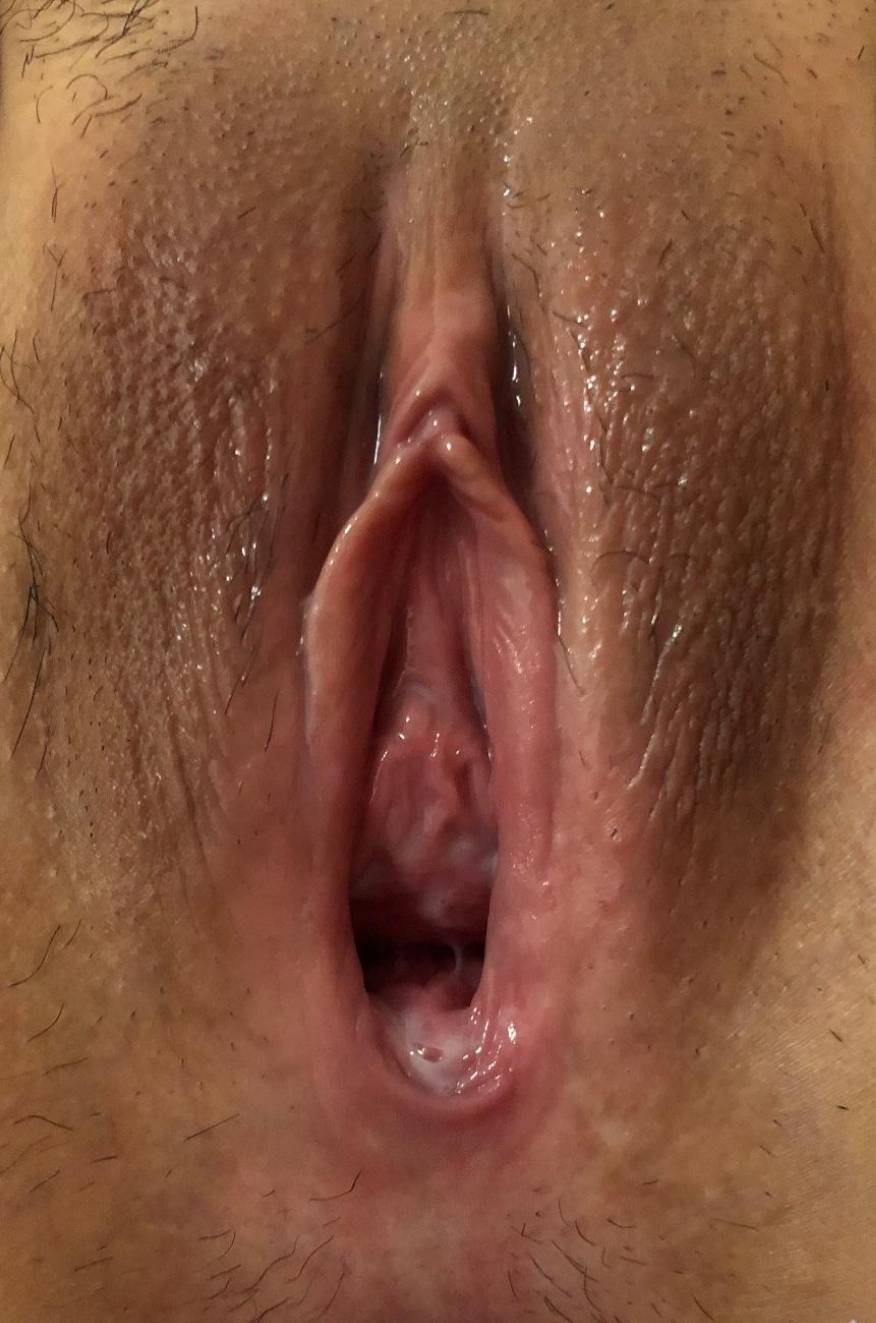
\includegraphics[width=0.85\textwidth]{images/fig_female_genital_anatomy.jpg}\\[0.4em]
{\small\itshape 图：女性外生殖器官（外阴）解剖示意，图中标注了外阴各主要结构。}\\[0.3em]
{\footnotesize 下列 1--5 各点即逐一对应图中结构，可对照查看。}
\end{center}
\par\smallskip

1．阴阜：耻骨联合前方的皮肤隆起，皮下具有较多的脂肪组织。性成熟期以后，皮肤长有阴毛。

2．大阴唇：一对纵长隆起的皮肤皱襞。大阴唇的前、后端左右互相联合，形成唇前联合和唇后联合。

3．小阴唇：位于大阴唇内侧，为一对薄的皮肤皱襞，表面光滑无阴毛。两侧小阴唇后端互相联合形成阴唇系带。

4．阴道前庭：位于两侧小阴唇之间的裂隙。前部有尿道外口，后部有阴道口，另外还有以下各部：

（1）前庭球：相当于男性的尿道海绵体，具有一定的勃起性。

（2）前庭大腺（Bartholin 腺）：成对，位于\textbf{阴道口两侧、小阴唇后缘深处}（约 4 点和 8 点方位），黄豆大，开口于阴道口与小阴唇之间的沟。功能：\textbf{性唤起时分泌少量黏液，参与润滑}（不是主要润滑来源——主要润滑来自阴道壁渗出）。常见临床问题（妇科门诊高频）：
\begin{itemize}[leftmargin=2em,itemsep=0.2em]
  \item \textbf{前庭大腺囊肿}：腺管堵塞、分泌物潴留形成\textbf{无痛性肿块}（阴唇一侧鼓起），小者可观察；\textbf{反复或增大者需就医}。
  \item \textbf{前庭大腺脓肿}：囊肿继发感染，\textbf{红、肿、热、痛}，可致\textbf{发热}、行走困难——\textbf{需切开引流}，别自行挤压（易扩散）。
  \item \textbf{反复发作}：可考虑\textbf{造口术（marsupialization）}或腺体切除，遵妇科建议。
\end{itemize}

5．阴蒂：由两个阴蒂海绵体构成。相当于男性的阴茎海绵体，表面盖以阴蒂包皮。露于表面的为阴蒂头，感觉敏锐。\textbf{阴蒂是女性最主要的性快感器官}——阴蒂头富含神经末梢（约 5000--8000 条，密度居全身之最），且内部海绵体远长于露在外面的一小截（向盆腔内延伸）；\textbf{多数女性的高潮依赖阴蒂刺激}（而非仅靠阴道插入），这也是 B 册反复强调"阴蒂刺激是核心"的解剖基础。

内生殖器

1．卵巢：卵巢是成对的实质性器官。呈扁卵圆形。卵巢位于子宫两侧，含有卵泡，是卵泡发育的部位。

卵泡由卵母细胞和卵泡细胞构成。原始卵泡位于皮质的浅层。卵泡在发育过程中体积长大，细胞数量增多。

周围结缔组织发生变化，卵泡的功能也相应变化。青春期以前，卵巢内仅有原始卵泡，进入青春期，原始卵泡在垂体的促性腺激素作用下，周期性的分批生长发育、成熟并排卵。每个月经周期有多个卵泡进入发育阶段，但一般只有一个卵泡发育成熟，其他卵泡都在发育的不同阶段退化成为闭锁卵泡。卵泡的发育是一个连续的过程。

原始卵泡：由位于中央的初级卵母细胞和周围单层扁平的卵泡细胞构成。

生长卵泡：生长卵泡又可分为初级卵泡和次级卵泡两个阶段。

1.初级卵泡：生长卵泡发育的初级阶段。

2.次级卵泡：卵泡细胞间形成充满卵泡液卵泡腔，这样的卵泡为次级卵泡。

3.成熟卵泡：卵泡体积明显增大，颗粒层变薄，整个卵泡突出于卵巢的表面。于排卵前36～48小时，初级卵母细胞完成第一次成熟分裂，产生一个大的次级卵母细胞和一个小的第一极体。次级卵母细胞随即进行第二次成熟分裂，并滞留于分裂中期。

出生时，初级卵泡的数量为15万～50万个。到青春期后逐渐减少，约34000个，到绝经期则所剩不多。在一个妇女的生育时期中，估计仅有300至400个卵细胞成熟排出，剩余以闭锁形式消失。成熟卵的直径为0.2毫米，是人体最大的细胞。在正常情况下，每个周期中只选择1个卵泡排卵，其余十几个较大的卵泡退化。

成熟卵泡破裂，次级卵母细胞连同透明带、放射冠与部分卵泡液一起从卵巢排出，进入腹腔的过程，称为排卵。次级卵母细胞由卵巢排出后，如果在24小时内不受精即退化；若卵受精。次级卵母细胞迅速完成第二次成熟分裂，形成一个成熟的卵细胞和一个第二极体。

通常每28天左右（即一个月经周期）排一个卵，双侧卵巢交替排卵。排卵一般发生在下次月经来潮前的14天左右。

排卵后，卵泡壁塌陷，在黄体生成激素（LH）的作用下，颗粒层细胞和卵泡膜内层的细胞分裂增生，形成一个血管丰富，具有内分泌功能的细胞团，新鲜时呈黄色，称黄体。排卵后7～8天，黄体发展到顶峰。

若排出的卵细胞未受精，在排卵后第10天黄体开始退化，黄体仅维持2周，称月经黄体；最后结缔组织取代成为白体。若排出的卵细胞受精，在胎盘绒毛膜促性腺激素的影响下，黄体进一步增大，6个月后才退化，称妊娠黄体。

2．阴道：处女期。阴道壁处于紧密相对的位置，其间形成一个潜在的腔，前壁长度范围6～7.5厘米。后壁大约9厘米。阴道腔在入口处收缩，中部扩张，接近子宫末端部分狭窄。子宫颈突入阴道腔，包绕宫颈的隐窝称阴道穹隆，分为前、后和侧部。

阴道壁由三层组成：粘膜、肌肉和纤维层。肌肉有两层：强韧的表面纵肌层。其纤维和子宫肌纤维相连；较弱的内环肌层，阴道被横纹肌纤维带所包围，外层结缔组织包围了肌肉组织。是膀胱直肠及其他骨盆结构的结缔组织的延续。

3．输卵管：输卵管是一对细长而弯曲的管道，全长约8～14厘米。输卵管位于子宫底的两侧，外端口开口于腹膜腔，内端开口于子宫腔，称输卵管子宫口。输卵管由内侧向外侧分为：子宫部、输卵管峡部、输卵管壶腹部、输卵管漏斗部。

4．子宫：子宫是一空腔器官，位于膀胱与直肠之间。它的形状是三角形。在妇女生育年龄期长6.5～8厘米，厚2.5～3厘米，底部宽5～6厘米，峡部宽2.5～3厘米。子宫体和子宫颈是连续的。在子宫底部侧面与输卵管相连。子宫腔下部与阴道连接；上部与输卵管腔相通。子宫内部为粘膜表面，称为子宫内胰。在这层之下为子宫肌层。由三层分界不清楚的平滑肌层组成。

子宫内膜组织及其分泌物在生殖过程中起主要作用。当精子通过子宫腔到达输卵管时，它们被浸泡在子宫内膜分泌物中。当受精卵运行到子宫腔，在着床之前的这一时期内。

它们又从子宫分泌物中接受营养。着床后胚胎依靠子宫内膜获得足够的血液供应以得到营养。以后子宫内膜的生理特点以及其血液供给足，胚胎在整个妊娠期的生存与发育的关键因素。

女性生殖生理

1．卵巢的功能：

卵巢是女性的生殖腺，具有产生并排放卵子和分泌雌激素、孕激素以及少量雄激素的功能。卵巢中卵泡发育经历原始卵泡、生长卵泡和成熟卵泡三个阶段，通过排卵过程卵细胞进入输卵管。雌激素由卵泡的颗粒细胞、内膜细胞和黄体细胞分泌，孕激素由黄体细胞分泌。

（1）雌激素：促进女性性器官的生长发育并维持正常状态，使子宫内膜发生增殖期变化。使宫颈腺分泌大量稀薄的粘液，促进输卵管运动，刺激阴道上皮细胞增生，降低阴道pH值，抑制病菌生长。促进女性性征的出现并维持于成熟状态。促进乳腺导管上皮增生。促进蛋白质合成，加速骨生长，促进钙盐沉积。促进肾小管对水和钠的重吸收。

（2）孕激素：通常在雌激素作用的基础上保证受精卵着床和维持妊娠；使子宫内膜在增殖期出现分泌期的改变，使宫颈腺分泌粘稠的液体。促进乳腺腺泡和导管的发育为分娩后泌乳做准备；排卵后由于孕激素的作用使基础体温升高0.2℃～0.5℃。

（3）下丘脑-垂体-卵巢轴调节：下丘脑分泌的促性腺激素释放激素经垂体门脉运送到腺垂体，作用于促性腺激素细胞，促进卵泡刺激素和黄体生成素的分泌。卵泡刺激素主要促进卵巢中卵泡的生长、发育和成熟，并在黄体生成素的协同作用下促使卵泡分泌雌激素。

黄体生成素则促使成熟卵泡排卵，使排卵后卵泡中残留的细胞转化为黄体细胞形成黄体，并促使黄体分泌孕激素和雌激素。

卵巢分泌的雌激素进入血液循环后，对下丘脑和腺垂体分泌的调节既有正反馈作用，也有负反馈作用，即在不同时期表现为促进其分泌或抑制其分泌。卵巢分泌的孕激素与雌激素协同对下丘脑和腺垂体的分泌产生负反馈作用，抑制其激素的分泌。

2．月经周期：

由月经来潮的第一天至下月月经来潮的前一天所经历的时间称为一个月经周期，平均28天，在月经周期中，子宫内膜经历周期性的剥脱、出血、修复和增生，按子宫内膜变化分为月经期、增生期和分泌期三期。

3．胎盘的内分泌功能：

（1）受精后第6天左右，胚泡形成滋养层细胞，开始分泌人绒毛膜促性腺激素，妊娠早期形成绒毛后由合体滋养层细胞分泌大量人绒毛膜促性腺激素，至妊娠8～10周分泌达高峰。此后下降并维持至分娩。人绒毛膜促性腺激素从尿中排出，可用于早期妊娠诊断。人绒毛膜促性腺激素在妊娠早期刺激母体的月经黄体转变为妊娠黄体，妊娠黄体分泌大量孕激素和雌激素以维持妊娠的顺利发展。

（2）由胎盘合体滋养层细胞分泌的胎盘催乳素，可促进乳腺发育，具有催乳作用，可调节母体的糖代谢和脂肪代谢，促进胎儿生长。

（3）妊娠期产生大量的甾体激素，主要有孕激素、雌激素和肾上腺皮质激素三类，胎盘不能独立合成这些激素，而是从胎儿或母体获取激素的前体物质进行加工。孕激素主要是孕酮，随着妊娠进展，孕酮分泌逐渐增加，足月时达高峰：孕酮使子宫内膜分泌，防止妊娠子宫收缩，对维持妊娠起重要作用。雌激素主要生理作用是促进子宫、乳腺发育增长，松弛骨盆韧带，调节母体和胎儿代谢。




男性生殖器官卫生


男性要注意阴囊、阴茎和睾丸的卫生。

阴茎

阴茎的表皮薄，皮下无脂肪。在不勃起时，阴茎的部分皮肤在冠状沟处复迭并遮盖阴茎头的后半部，即包皮。包皮内面和阴茎头连接处有小皮脂腺不断地分泌淡黄色的油性物质，与少量的尿液和皮肤脱下来的污垢混合成包皮垢。包皮垢很容易为细菌繁殖造成机会，引起发炎等。因此，阴茎和包皮应当勤洗以免积垢较多，发生不适或感染。

包茎和包皮过长是常见的包皮发育异常。包茎指包皮口狭窄或包皮与阴茎头粘连，包皮不能上翻露出尿道口和阴茎头。小儿一般到三岁以后阴茎头和包皮之间的轻度粘连才自行消失。童年时包皮能上翻但也常将尿道口盖住，在青春期阴茎头逐渐露出。因此，在童年以前包皮长是正常的。成人阴茎疲软时包皮不遮盖尿道口。包皮上翻时能露出冠状沟，即为正常长度的包皮。包茎严重可影响排尿，以致造成整个泌尿系统的机能障碍。包茎和包皮过长会减低男方性快感，甚至因包皮牵扯可感觉疼痛。包皮过长要保持局部清洁，经常清洗，最好行环切术。因为屡次炎症可使包皮口缩小，并与阴茎头形成粘连，变为包茎。包茎也可为后天获得。包茎时包皮垢易引起慢性炎症，甚或诱发癌变。包茎可以手术治疗，包皮过长一般也以手术切除为宜。

阴囊和睾丸

阴囊是皮肤囊袋，内容睾丸、附睾等。阴囊可随温度的变化而发生变化。常态下阴囊多处于收缩状态，表面出现皱褶。当温度增高时或在老年人以及体弱者，阴囊常伸展呈松弛状态，皱褶消失。在寒冷的环境中，或在青年人以及强壮者，阴囊缩小并与睾丸紧贴。阴囊的收缩或舒张，可以调节阴囊内的温度，以适于精子的生长和发育。阴囊的皮肤薄而柔弱，因此应避免伤害。不要用碘酒及一些刺激性较大的药物，小心避免虫咬等等，以免造成疼痛和损伤。

睾丸约在胚胎第7～9月内降入阴囊。个别孩子出生时未降入，亦多在出生后短期内降入。未降入阴囊的睾丸称为隐睾，隐睾多数发生在右侧，也有发生在双侧。隐睾对睾丸功能的影响在5岁以后逐渐开始，主要是曲细精管萎缩，导致精子生长不良。青春期后，绝大多数隐睾者发生睾丸萎缩，如果发生在双侧，则丧失生育能力，并出现雄激素缺乏的症状。另外，隐睾发生肿瘤的机会较正常的要大数十倍。因此，隐睾需要积极治疗。单侧隐睾多需手术治疗。双侧隐睾可先用药物治疗，效果不满意者再考虑手术。一般在5～6岁前施行手术，最迟不应晚于10岁，否则睾丸的发育障碍不能恢复。

成年睾丸如鸽卵大小。一般左侧的睾丸比右侧的大一些，也比右侧低一些。睾丸表面有一层光滑的膜，使睾丸在阴囊里可以自然滑动，在剧烈运动时，也不至于受到损伤。但易受暴力的挤压和打击，使睾丸受到严重损伤。





女性生殖器官卫生


因为女性要妊娠和分娩，因此女性生殖器官在结构和生理上，都比男性复杂。

女性生殖器的自然防御机制

女性的阴道口距肛门很近，很易造成污染。但是阴道的外侧端比内侧端狭窄，平时阴道的前后壁是互相紧贴，使阴道口闭合着。另外。阴唇亦有一定的保护作用，因而阻挡了部分病原体侵入阴道内。阴道上皮细胞在卵巢分泌的性激素作用下增生、表层细胞角化，使阴道粘膜得以抵抗阴道内的病原体侵入了。子宫颈内口平时是紧闭的。

子宫颈管形成粘液栓，阻止病原体进入子宫腔内。子宫内膜周期性的剥脱，也可以清除子宫腔内的部分污物和病原体。阴道在正常情况下呈酸性环境。抑制了在碱性环境下繁殖的病原体，而子宫颈管的粘液呈碱性，使适应于酸性环境的病原体的繁殖受到抑制，便可保持相对清洁和卫生。在一般情况下，过多地清洗阴道将会破坏阴道内和子宫颈管的正常酸碱平衡，使原来受到抑制的病原体生长和繁殖活跃起来，以至引起阴道、宫颈、官腔、输卵管等器官的炎症。

当妇女体弱多病时，免疫功能就下降。营养充分、健康良好时，免疫功能的作用就较强。因此，性器官也依赖于身体的整体健康水平。

阴道分泌物

阴道分泌物是由阴道粘膜渗出物、宫颈腺体及部分来自子宫内膜的分泌物混合而成，内含阴道上皮脱落细胞、白细胞、乳酸杆菌，医学上将这些统称为“白带”。

正常情况下的自带为白色粘稠物，一般无气味，量多少不等，与雌激素水平高低及生殖器官充血情况有关。青春期卵巢逐渐发育，并分泌雌激素时，开始有阴道分泌物排出，一般在月经中期接近排卵期时，由于宫颈内膜腺细胞分泌旺盛，白带中的宫颈粘液占主要成分，此时白带增多，清澈透明，稀薄似鸡蛋清。排卵2～3天后，白带又变成混浊粘稠而量少。行经前后因盆腔充血，使阴道粘膜渗出物增加，白带也往往增多。妊娠期因雌激素水平高，阴道粘膜渗出物及宫颈分泌物都增加，故白带也较多。另外，性生活前后、阴道内使用避孕药物等，都可能引起白带增多。

当妇女身体出现不适时会有白带异常。特别是发生生殖器官的炎症或癌症时。白带异常主要有：

1．无色透明粘性白带外观与正常白带基本相似，只是量比较多，常见于应用雌激素类药物，或使用阴道避孕药之后，妇女体虚亦可见这种白带。

2．血性白带内混有血，血量多少不定，应进一步检查恶性肿瘤的可能，如宫颈癌、宫体癌等。另外，如宫颈息肉，宫内节育器所引起的副反应。粘膜下肌瘤，老年性阴道炎，重度慢性宫颈炎等也可出现血性白带。

3．豆腐渣样白带呈豆腐渣样或凝乳状小碎块，为霉菌性阴道炎所特有，常伴有外阴瘙痒。

4．脓性白带色黄或黄绿有臭味，大多为滴虫或化脓性细菌感染所引起，常见于滴虫性阴道炎、慢性宫颈炎、老年性阴道炎、子宫内膜炎、宫腔积脓、阴道异物等。

5．黄色水样白带往往是由于病变组织坏死或变性所致，常发生于子宫粘膜下肌瘤、子宫颈癌、子宫体癌、输卵管瘤。黄色水样白带量多而带有恶臭味者。应注意作进一步检查确定病因并进行治疗。

外阴的卫生

妇女要经常清洗阴阜和大阴唇。因为自阴道内流出的自带、月经血和外阴分泌物粘附在阴毛内，或积存在大阴唇同小阴唇、阴蒂之间的皱褶中。如果不经常清洗掉，便可刺激外阴的皮肤，引起瘙痒或炎症。这些污垢也增加了病原体进入阴道口的机会。清洗外阴的顺序是：从大阴唇内侧开始，向内清洗小阴唇、阴蒂周围及阴道前庭。尿道口处于阴蒂下方及前庭前部，其后上壁有一对并列的腺体，称尿道旁腺，常为细菌潜伏所在，故尿道口、阴道口周围应注意清洗。然后，清洗大阴唇外侧、阴阜、大腿根部内侧，最后清洗肛门。

女性的内裤要经常换洗，洗外阴和内裤应有专用盆。妇女要避免内裤穿得太紧。女性的尿道比较短，距阴道口很近，阴道口生长繁殖的病原体也时刻威胁着尿道口，这些病原体一旦进入尿道，就可能沿着尿路上行感染引起泌尿系统的炎症。另外，肛门距外阴也很近，如果内裤穿得太紧，内裤便与外阴和肛门频繁地摩擦，肛门处的病原体可以通过内裤污染到外阴，同时，内裤与外阴的紧贴摩擦，帮助了外阴处的病原体进入尿道口和阴道口，引起泌尿系或生殖系的感染。

月经期的卫生

月经周期一般为28～30天，提前或延后7天左右仍属正常。每人月经周期有自己的规律性。月经可持续2～7天，多数为3～5天。月经量一般在50毫升左右，个别妇女可超过100毫升或量很少，月经的第2～3天出血量最多。大多妇女在月经期无特殊症状。有些妇女可有下腹部下坠及腰部沉重，个别可有尿频、轻度头痛、失眠、精神抑郁、易于激动、肠胃功能紊乱如恶心、呕吐、便秘或腹泻以及鼻粘膜出血等。

由于月经期生殖器官及全身神经体液等方面有较大变化，如不注意保护身体，不讲究卫生，便有可能引起妇科疾病。

有些人认为月经血很脏，不愿用手去碰，于是在月经期间便不清洗外阴，甚至有的人不注意卫生巾的清洁，不按时更换卫生巾，这都是不正确的做法。积存在阴道内、粘附在外阴上、渗透在卫生巾上的血液，是病原体生长繁殖的地方，因此，要及时清洗外阴和内裤，要用干净的盆和干净的毛巾蘸温水擦洗外阴，从前面到后面，不要将外阴浸泡在水中，以免污水进入阴道内。

月经期前后，阴道的酸碱度有所变化，经期子宫口微微张大。因此，生殖器官的炎症常在此期复发或加重，必要时，可适当地用药。

由于失血、机体抵抗力下降，月经期不宜进行重体力劳动或剧烈运动，应避免接触冷水，饮用、食用冰冻食品和饮料，月经期间应禁止性交以免感染。

\chapter{妇女保健及病症治疗}


女性不宜留长发


长发是女性人为的外部特征之一。长发飘飘虽然美丽，但却影响女性智力。现代医学和化学测验表明，人的头发中含铁、碘、锌和各种维生素等等人体必需的几十种营养成分，从一根头发之中，可以测得人的血型，验得血液中各种营养成分指标，这一切都说明了头发吸收了人体的各种营养。

人被头发所消耗掉的营养难以计算，人体供给头部的营养既然过多地被头发所吸收，那么，脑部营养自然就要相对地减少，以至于导致脑部营养的缺乏，而脑部营养的缺乏，又会导致头晕现象的不断发生，直接影响人的智力的发展。在一般情况下，女性比男性头晕病患者多，这其中长发姑娘所占比例大于短发姑娘。





女性不宜长期紧衣束腰


女性的尿道具有短、宽、直和肌肉力量薄弱等特点。成年女性尿道平均长度是3.5厘米，而短于3厘米的尿道便不能阻止尿液外流，很自然有些尿道过短的女性会发生尿失禁。现在，喜欢穿紧身衣裤和扎紧束腰带的越来越多。日子一长，她们的膀胱就会被压向前下方，致使尿道与膀胱连接处的后角增大变直，这样便不利于排尿的控制，在奔跑、弯腰、剧烈咳嗽、打喷嚏、哈哈大笑等情况下，尿液便会不由自主地流出来，这当然令人既痛苦又烦恼。因此，年轻女性紧身衣裤不要穿得时间过长，腰带也不要束得太紧，要与宽松裤交替穿才是。





妇女生育有益心脏


美国心脏学会研究人员认为，女性生育对心脏之所以产生保护作用，也许是女性激素起的作用。特尔弗教授认为，如果这被证实，那么，那些死于心脏病的产育妇女，可能正是缺乏某种特定保护性激素，因而一方面影响了生育，同时对心脏也减少了保护。





妇科疾病总概


女性生殖系统的疾病即为妇科疾病，包括外阴疾病、阴道疾病、子宫疾病、输卵管疾病、卵巢疾病等。妇科疾病是女性常见病、多发病。但由于许多人对妇科疾病缺乏应有的认识，缺乏对身体的保健，加之各种不良生活习惯等，使生理健康每况愈下，导致一些女性疾病缠身，且久治不愈，给正常的生活、工作带来极大的不便。





闭经


闭经是许多妇科疾病所共有的一个症状，是由下丘脑-垂体-卵巢轴中的某一环节发生功能或器质性病变引起。按引起闭经的病变部位，可分为子宫性、卵巢性、垂体性和下丘脑性闭经。妇女年满18周岁经尚未来潮称为原发性闭经，约占闭经总数的5％，多为先天发育异常，月经已经来潮，而出现连续6个月月经不行者。称为继发性闭经，约占95％，病因各异。中医学将本病称之为“女子不月”、“月事不来”、“血枯”、“血隔”。

【临床特征】

已年满18周岁月经尚未来潮，或月经已来潮又连续6个月未行经。或伴有头痛、视力障碍、恶心、呕吐、周期性腹痛；或有多毛、肥胖、溢乳等。

【医生诊断】

1．有典型症状。

2．全身检查。注意一般发育及营养状况、精神神经类型、智力水平、有无躯体畸形。必要时测量身高、体重、指距及第二性特征发育情况，有无肥胖、多毛、溢乳等。

3．妇科检查。注意外阴发育和阴毛分布情况，有无阴蒂肥大，阴道发育情况，阴道、处女膜有无梗阻、畸形、萎缩，子宫有无及大小，卵巢是否增大。

4．子宫检查。

（1）官腔镜检查：了解宫腔深度、宽度、形态有无畸形，有无粘连，取内膜检查有无病理改变。

（2）腹腔镜检查：直视子宫及性腺外观，除外先天发育异常，必要时取卵巢活检。

（3）子宫输卵管碘油造影：了解官腔形态，有无畸形，输卵管是否通畅，除外结核病。

（4）药物试验检查：孕激素和雌激素试验，观察子宫内膜有无反应。

5．卵巢功能检查。

（1）阴道黏液结晶检查：了解雌激素水平。

（2）宫颈黏液结晶检查：了解雌激素水平及有无孕激素影响。

（3）基础体温测定：了解有无排卵及黄体功能。

（4）雌孕激素水平测定：了解卵巢功能。

6．垂体功能检查。

（1）测定血中 FSH、LH 含量：若高于正常水平提示卵巢功能低下；若低于正常水平表示垂体功能或更高中枢功能低下。

（2）垂体兴奋试验：一般用药后 15～30 分钟，LH 值高于用药前的 2～4 倍，为垂体功能良好。如不升高或升高很少说明病变可能在垂体。

（3）血中催乳素测定：如 PRL＜$50\,\mu\mathrm{g}/\mathrm{L}$，应进一步作 PRL 兴奋或抑制试验，以鉴别 PRL 的功能性分泌增多与垂体腺瘤。

（4）蝶鞍X线片、CT、核磁共振等检查：以除外垂体肿瘤。

7．染色体检查：除外性发育异常。

【西医诊疗】

（1）一般治疗。对因环境改变、精神创伤引起的一时性闭经，可通过加强营养，增强体质，避免精神紧张及过度劳累等予以调整。对口服避孕药引起闭经者，应停药观察。

（2）子宫内膜结核者。予以抗痨药物治疗。

（3）内分泌治疗。适用于先天性腺发育不良、卵巢功能受损、垂体功能低下、卵巢功能早衰等引起的闭经。

1.雌激素治疗、孕激素治疗、雌孕激素治疗等。

2.诱发排卵：可选用克罗米酚、绒毛膜促性腺激素、促性腺激素释放激素等。但必须在B超监测下使用，防止出现卵巢过度刺激综合症。

（4）手术治疗。

1.宫腔粘连者，扩张宫颈，分离粘连，并放置宫内节育器以防再粘连。

2.对卵巢、垂体及其他部位的肿瘤可行手术治疗。

【中医用方】

（1）肾气不足：原发性闭经，或初潮晚，月经错后量少，色淡黯质稀，渐至闭经，头晕耳鸣，腰膝酸软，夜尿频，带下少，面色晦暗，舌质淡、苔薄润，脉沉细无力、尺脉弱。方法：补肾益精，调补冲任。

用药：菟丝子、首乌、黄精、枸杞子、熟地、覆盆子、党参、当归、女贞子各15克，紫河车、仙灵脾、肉苁蓉各10克。

参考中成药：参茸丸。

（2）肝肾亏损：堕胎、流产、久病或产后，经量逐渐减少，经行延后。渐至闭经，头晕目涩，腰膝酸软，心烦潮热，带下量少，阴部干涩，甚则形体消瘦，面色萎黄，肌肤不润，毛发脱落，性欲淡漠，舌质淡、苔薄白或薄黄，脉细无力。

方法：滋补肝肾，养血填精。

用药：枸杞子、首乌、当归、熟地、山药、女贞子、茯苓各15克，山萸肉12克，杜仲、菟丝子、巴戟天各10克。参考中成药：妇科金丸。

（3）气血虚弱：月经逐渐后延，经量渐减，色淡质稀，继而停闭，倦怠乏力。气短懒言，头晕眼花，心悸失眠，毛发少泽，肌肤欠润，舌质淡、苔薄白，脉细弱。方法：益气养血调经。

用药：白术、茯苓、党参、炙黄芪、当归、白芍、熟地各15克，远志、炙甘草各10克，陈皮、桂圆各6克。

参考中成药：八宝坤顺丸、乌鸡白凤丸。

（4）气滞血淤：经行先后不定，量少，渐至闭经，或暴怒之后骤然经闭不行，情志抑郁，胸胁、乳房、少腹胀痛，舌质黯或有淤斑淤点、苔薄白或薄黄，脉弦涩。

方法：理气活血，祛淤通经。

用药：当归、赤芍、川牛膝、莪术、熟地各15克，桃仁12克，红花、枳壳、醋柴胡、桔梗、川芎、甘草各10克。

参考中成药：血府逐淤丸。

（5）痰湿阻滞：经期延后，经量渐少而至停闭，神疲倦怠，形体渐胖，胸脘满闷，食少痰多，带下量多，色白质稠，舌质淡胖、苔白腻，脉滑。

方法：燥湿化痰，活血通经。

用药：苍术、当归、茯苓各15克，半夏、陈皮、神曲、川芎、生甘草、制香附、胆南星、枳壳各10克，生姜3片。

参考中成药：二陈丸。

【预防和调养】

1．积极治疗月经后期，月经量少等疾病，以免病情进一步发展，导致闭经。

2．保持心情舒畅，避免过度精神紧张，减少精神刺激。

3．调节饮食，注意蛋白质等营养物的摄入，避免过分节食或减肥。造成营养不良引发此病。

4．注意经期及产褥期保健，勿冒雨、涉水、过劳等。





更年期综合症


【概述】

更年期是指妇女45～55岁的阶段，由生育期过渡到老年期的一个必经的生命阶段，它包括绝经前期、绝经期和绝经后期。绝经前期临床表现为月经周期不规则，出现各种精神、神经症状；绝经期月经完全停止，持续时间应在1年以上，精神、神经症状持续存在；绝经后期，除精神、神经症状外，还出现因雌激素缺乏和年老所引起的各种器官系统的症状。症状持续时间一般为2～5年，甚或更长时间，个体差异很大。其根本原因是由于卵巢功能衰退而导致下丘脑-垂体-卵巢轴内分泌功能紊乱，出现雌孕激素明显降低，而促性腺激素明显升高所致，另外还与社会，文化因素和妇女自身个性等因素有关。所以更年期综合症是由内分泌、社会文化及精神三种因素互相作用的结果。中医学称之为“绝经前后诸症”。

【临床特征】

1．血管舒缩综合症。表现为潮红、潮热、出汗、心悸、眩晕等。潮红发作频率及持续时间有很大差异，有的偶然发作，有的每天数次或数十次，持续时间数秒至数分钟不等。

2．精神、神经症状。主要表现为忧虑、记忆力减退、注意力不集中、失眠、极易烦躁，甚至喜怒无常等。

3．月经紊乱是更年期综合症主要表现，有三种形式。

（1）月经周期延长或间歇闭经，月经量和行经时间逐渐减少变短，最后致月经停止而绝经，这是最常见的形式。

（2）月经周期缩短、频发，月经量多，甚至出现阴道大出血，经期延长或淋漓不止，以后逐渐减少至绝经。

（3）月经突然停止，但较为少见。

4．生殖器变化。

（1）阴道：阴道萎缩，弹性消失，出现性交疼痛及困难，阴道黏膜变薄，糖原减少易致老年性阴道炎，白带增多，色黄有味甚至带血，阴道烧灼疼痛。

（2）宫颈：萎缩变小，有时子宫颈管闭锁而发生子宫积脓。

（3）子宫；由于盆底肌肉及韧带松弛也可出现子宫脱垂，阴道前后壁膨出。

5．尿道。雌激素减少使尿道萎缩、狭窄、括约肌松弛，出现尿频、尿急、尿失禁、排尿不畅、尿潴留等。

6．皮肤与毛发。皮肤出现皱纹，手背、面部可见褐色老年斑，毛发脱落并逐渐变白。

7．骨与关节。雌激素水平低下致骨钙量快速丢失，导致发生绝经后骨质疏松症。

8．心血管病变。出现更年期高血压，特别是以收缩压升高力主，波动大。还可出现“假性心绞痛现象”，患者自觉心前区痉挛感，心悸、阵发性心动过速或过缓。

【医生诊断】

1．年龄45～55岁的妇女，除月经失调外，烘热汗出为典型症状，或伴有烦躁易怒，心悸失眠，胸闷头痛，情志异常，记忆力减退，腰腿酸痛等。

2．内分泌测定。雌二醇降低，促卵泡激素、促黄体生成激素增高。

3．应排除精神、神经性疾病，甲状腺机能亢进，心血管疾病等。

【西医诊疗】

（1）一般治疗：更年期妇女出现一般症状只需予以解释、安慰、消除顾虑，同时积极安排好工作和生活。若出现明显症状，如头痛、失眠等精神症状，可给予镇静剂，如安定、谷维素等，血压增高可给降压药，均能减轻症状。

（2）激素替代疗法：一般选用雌激素替代治疗。

1.二醇：每日1～2毫克或雌二醇每日阴道内用0.5毫克，每月连用24～26日，周期性加用孕激素，如炔诺酮每日0.5～1毫克，或安宫黄体酮6～10毫克，每月用7～10日，常诱发周期性出血。

2.雌、孕激素联合应用：雌激素用量同前，孕激素用量为前述量的1/3～1/2。或乙炔雌二醇每日50微克，安宫黄体酮每日2微克，二者隔日交替使用，一般不导致突破性出血。

3.尼尔雌醇：每次1～2毫克，每2周1次，3个月后加用安宫黄体酮每日6～10毫克，每日共7～10，有撤退出血者每3个月重复1次，否则改为每6个月重复使用。

4.利维爱：每次2.5毫克，每日1次。但在使用以上药物时，应掌握适应症，治疗前应除外子宫肌瘤、子宫内膜癌、乳腺肿瘤，肝、肾及胆道疾病、血栓性静脉炎等，用药期间定期检查乳腺、阴道、宫颈、子宫、肝功、血压等。

【中医用方】

（1）阴虚血燥：经断之年，头晕耳鸣。腰臃酸软，肢体麻木、瘙痒或有蚁行感，皮肤干燥，阴部干涩。大便干燥，舌质红、少苔，脉虚细数。

方法：滋阴养血，润燥祛风。

用药：生熟地、山萸肉、枸杞子、山药各15克，菟丝子、生首乌各20克，当归、白芍各12克，丹皮10克，炒荆芥6克，蝉衣3克。

参考中成药：左归丸。

（2）精亏血枯：经期前后，腰膝酸软，头晕耳鸣，失眠健忘，甚则齿摇发脱，月经过早停闭，或后期量少，舌淡、苔薄，脉细弱。

方法：滋肾填精养血。

用药：枸杞子、熟地、山药、狗脊、制首乌、当归、菟丝子各15克，山萸肉12克，鹿角胶（烊）、龟板胶（烊）、川牛膝各10克。

参考中成药：左归丸。

（3）肾虚阴旺：经断前后，烘热汗出，烦躁易怒，头晕耳鸣，腰膝酸软，双目干涩，舌质红、少苔，脉细弦数。

方法：滋肾养肝，平肝潜阳。

用药：枸杞子、山药、熟地、茯苓、白芍、石决明各15克，丹皮、菊花各10克，山萸肉12克，制鳖甲（先下）20克，生龙牡（先下）各30克。

参考中成药：天王补心丹，交泰丸。

（4）肾阳虚：绝经前后，腰背酸冷，精神萎靡，形寒肢冷，小便清长，夜尿频，或面浮肢肿，纳呆便溏，甚者五更泄泻，或经行量多，崩中漏下，经色淡暗，舌质淡、苔薄白，脉沉细弱。

方法：温肾扶阳。

用药：熟地、山药、枸杞子、菟丝子、仙灵脾各15克，山萸肉12克，鹿角胶（烊）、杜仲、覆盆子各10克，肉桂6克。中成药；右归丸。

【预防和调养】

1．加强卫生宣传教育，使更年期妇女了解保健知识，正确对待更年期。

2．保持心情舒畅、开朗，克服内向、拘谨、抑郁、多虑等不利心理因素，减少发病。

3．注意生活调护，劳逸结合，饮食有节。

4．积极参加适当的体育锻炼，增强体质，增强抗病能力。

5．维持适度的性生活，有利于心理、生理健康。





子宫肌瘤


【病症概述】

子宫肌瘤也称为“子宫纤维瘤”、“子宫纤维肌瘤”、“子宫平滑肌瘤”。它是女性生殖器官中最常见的良性肿瘤，主要由平滑肌和结缔组织构成，确切病因不清，多认为可能与长期和过度的雌激素有关。肌瘤多生长在子宫体部，少数生长于子宫颈部。当肌瘤增大或瘤体内发生栓塞时，易发生变性。多见于30～50岁妇女。中医学称之为“瘙瘕”。

【临床特征】

临床症状与肌瘤生长的部位、大小有关。月经改变为最常见的症状，较大的肌壁间肌瘤和黏膜下肌瘤多出现月经量多，经期延长和周期缩短，可伴有不同程度的贫血，黏膜下肌瘤时有不规则阴道出血，或白带异常。肌瘤增大时，可出现尿频、尿急或排尿困难等压迫症状，甚至能在下腹部自行扪及肿物。浆膜下肌瘤扭转或有肌瘤变性，可出现急性腹痛。部分患者可因肌瘤生长部位妨碍孕卵着床或影响精子的通行。还可导致不孕或流产。

【医生诊断】

1．具有典型症状，或部分患者无症状。

2．妇科检查：子宫增大，表面有不规则凸起，质硬，大肌瘤腹部即可触及肿块，当黏膜下肌瘤突出于阴道内，可见紫红色光滑的环形肿物，若肌瘤变性时，子宫变软，有压痛。

3．B超：是诊断子宫肌瘤最常用的检查方法，根据回声图像，可显示子宫大小，宫内情况，肌瘤的数目、大小、部位及退行变性等。

4．官腔探测或诊刮：可了解宫腔深度及形态。

5．子宫输卵管碘油造影：可显示子宫大小、官腔形态及肌瘤附着部位。

6．内窥镜检查：官腔镜可窥视腔内的黏膜下肌瘤，腹腔镜可直视子宫外形及肌瘤情况。

7．鉴别诊断

（1）妊娠子宫：根据停经史，妊娠反应，子宫增大变软，尿妊娠试验阳性等，与子宫肌瘤不难鉴别。若肌瘤合并妊娠时，可行B超协助诊断。

（2）卵巢肿瘤：一般二者不难鉴别，但实质性卵巢肿瘤可能被误诊为浆膜下肌瘤。反之浆膜下肌瘤囊性变时也易误诊为卵巢囊肿。当卵巢囊肿与子宫有粘连时。则更难鉴别，但B超和腹腔镜可确诊。

（3）子宫腺肌病：临床上也有月经量多、经期延长和子宫增大，但临床症状以痛经、进行性加重为主，检查时子宫呈均匀性增大，很少超过妊娠两个月大小，具有经前子宫增大、经后缩小的特征，B超能帮助诊断。当肌瘤与肌腺病同时存在，则不易鉴别，常需术后病理证实。

【西医诊疗】

（1）随访观察：如子宫肌瘤无症状，并小于3个月妊娠大小，月经正常，可每3～4个月复查1次。

（2）激素治疗：患者年近绝经期，因某种原因不适于手术治疗者，经内膜病检排除恶变后，可用雄激素治疗。甲基睾丸素，每次5～10毫克，每日1次；或丙酸睾丸酮，每次25毫克，每周肌注2～3次。每月剂量不超过300毫克。

（3）根据不同病情，选用手术治疗：刮宫术、腹式子宫肌瘤摘除术、经阴道子宫肌瘤摘除术、子宫切除术。

【中医用方】

（1）气滞血淤：胞中癥块，月经量多，经期延长，经色紫暗，有血块，小腹胀痛，血块下后痛减，经前乳房胀痛，情志抑郁或心烦易怒，舌质紫暗、苔薄白，脉弦涩。

方法：行气活血，消癥散结。

用药：当归、红花、三棱、莪术、乌药、川芎、桃仁、制香附各10克，赤芍、荔枝核、夏枯草各15克，生牡蛎30克，炙甘草6克。

参考中成药：五香丸。

（2）气虚血淤：胞中积块，月经先期量多，或淋漓不净，色淡、有血块，小腹坠痛，气短乏力，食少便溏，面色咣白，舌质淡暗、边有淤斑，脉虚细涩。

方法：益气补中，化淤消癥。

用药：炙黄芪、夏枯草、白术、党参、山药、山慈菇、昆布各15克，三棱、莪术、枳壳各10克。

参考中成药：妇科伺生丹。

（3）痰淤互结：胞中积块，小腹胀痛，带下量多，色白质稠，月经量多有块，婚久不孕，胸脘痞满，形体肥胖，舌质紧黠、苔腻，脉沉滑。

方法：理气化痰，祛痰消癥。

用药：茯苓、苍白术、夏枯草、海藻各15克，半夏、陈皮、制香附、川芎、槟榔各10克，莪术12克，木香6克。

参考中成药：桂枝茯苓丸合二陈丸。

【预防和调养】

1．调节情志，精神舒畅，保持气血平和。

2．清洁外阴，因子宫肌瘤常有经期延长，故应保持外阴清洁，防止感染。

3．合理应用性激素类药物，防止长期过量应用雌激素。

4．注意性生活的程度和频度把握。





卵巢良性肿瘤


【病症概述】

卵巢良性肿瘤为妇科常见肿瘤，种类较多，可发生于任何年龄，20～40岁为发病高峰。多数患者常无症状，生长缓慢，当出现症状时，肿瘤多已长大，病因不清，可能与环境因素、遗传因素等有关，中医学称之为“肠覃”、“癥瘕”。

【临床特征】

卵巢良性肿瘤生长缓慢，初期五症状，增大后下腹部可出现包块，患者感到下腹不适，坠胀，或尿频急，大便不畅，气短，静脉曲张，腿肿等肿瘤牵拉或压迫症状。当发生蒂扭转、破裂或感染，可出现急性腹痛。

【医生诊断】

1．具有上述症状或无不适感觉。

2．下腹部扪及囊性包块，多为圆形，大者可充满全腹，一般可活动。

3．妇科检查，子宫一侧或双侧触及圆球形囊性肿块，表面光滑，可活动。

4．B超可提示肿瘤的部位、大小、质地等。

5．腹部X线，可确诊畸胎瘤。

6．鉴别诊断

（1）子宫肌瘤、子宫肌瘤囊性变或浆膜下肌瘤有时需与之鉴别，可借助B超协助诊断。

（2）妊娠子宫，有停经史、妊娠反应、尿妊娠试验阳性，B超可确诊。

【西医诊疗】

（1）肿瘤直径＜5厘米者，密切随访，每3～6个月检查一次。

（2）手术治疗：为主要的治疗方法。根据年龄和肿瘤的性质，可以选择患侧肿瘤剔除术、患侧附件切除术、全子宫加双附件切除术等。

【预防和调养】

卵巢肿瘤的发生目前尚不能预防，但早期发现、及时处理则可防止其增长、变性，以及并发症的发生，并可保存卵巢功能，故应定期普查、普治。





不孕症


【概述】

夫妇同居2年，配偶生殖功能及性生活正常，未采取避孕措施而不受孕者，称为不孕症。分原发不孕和继发不孕，前者指婚后从未受孕；后者为曾生育或流产后，未避孕而又2年以上不再受孕。女方不孕因素包括：下丘脑-垂体-卵巢轴功能紊乱致无排卵，输卵管阻塞影响精卵结合，子宫发育不良或内膜病变影响受精卵着床，外阴、阴道或宫颈因素影响精子穿过。根据不孕的原因又分为相对不孕和绝对不孕，前者指引起不孕的因素可以得到纠正，仍有受孕可能者，后者指有先天或后天解剖生理方面的缺陷，无法纠正而不能受孕者。中医称原发性不孕为“无子”、“全不产”，称继发性不孕为“断绪”。

【临床特征】

结婚2年以上，或曾孕育2年以上，未避孕而不受孕。根据引起不孕原因的不同，可伴见月经失调、痛经、带下异常、盆腔炎症、内分泌失调等症状。

【医生诊断】

结婚2年以上，或曾孕育后2年以上，配偶生殖功能正常，性生活正常，未采取任何避孕措施而不受孕者，即可诊断为不孕症。

此外，通过全面的检查找出不孕的原因，即病因诊断，是治疗此病的关键。女方检查包括：详细询问病史，全面体格检查，卵巢功能测定，输卵管通畅试验，性交后试验，宫颈黏液、精液相合试验，腹腔镜，官腔镜检查等。以上检查需按计划、有步骤地进行。

【西医诊疗】

（1）一般处理：积极治疗全身性疾病，安排排卵期性生活，免疫性不孕者应用安全套避孕半年。

（2）内分泌治疗：

1.无排卵者给予克罗米芬50毫克，于月经第5天起口服，连续5天，停药后7天加用hCG2000～5000单位肌肉注射1次；或月经第6天每日肌注hMG1支共7天，停药后24～36小时加用hCG5000～10000单位肌注。高泌乳素血症无排卵者。口服澳隐亭1.25毫克，每日2次。

2.黄体功能不足者于月经第15天开始每日肌注hCG1000～2000单位；或于月经第20天每日肌注黄体酮20毫克，共5天。

3.甲状腺功能低下者或过度肥胖者，给予甲状腺素片。肾上腺皮质功能亢进者，应用地塞米松或强的松。

（3）抗炎治疗：严重的生殖道炎症患者应用抗生素治疗。

（4）手术治疗：处女膜闭锁、阴道横膈、宫腔粘连、输卵管阻塞及肿瘤，均可行手术治疗。

（5）人工授精，体外授精。

（6）由于男性原因引起，或者女性分泌液专杀精子者采取其他相关治疗。

【中医用方】

（1）肾阳虚：久不孕育，经行后期、量少、色淡、质稀，腰膝酸软，畏寒肢冷，夜尿频，舌质淡、苔白滑，脉沉细无力。

方法：温补肾阳，调经助孕。

用药：熟地、菟丝子、枸杞子、党参、白术、白芍、茯苓各15克，紫河车、鹿角霜、川椒、当归各10克。

参考中成药：河车大造丸。

（2）肾阴虚：婚久不孕，月经量少、色红、无血块，腰膝酸软，头晕耳鸣，口干，舌质红、少苔，脉细数。

方法：滋肾填精，调经助孕。

用药：熟地、山药、山萸肉、女贞子、菟丝子、白芍、黄精各15克。

参考中成药：安坤赞育丸。

（3）肝郁：婚久不孕，月经时先时后，经行不畅，色暗，有血块，经前乳胀、心烦，口干，胸胁胀满，舌质红、苔薄白，脉弦。

方法：滋阴补肾，调经助孕。

用药：醋柴胡、当归各10克，白芍、白术、茯苓各15克，薄荷（后下）3克，炙甘草、煨姜各6克。

参考中成药：逍遥丸。

（4）痰湿：婚久不孕，月经后期量少或经闭不行，形体肥胖，带多色白质稠，口淡黏腻，舌质淡、苔白腻，脉滑。

方法：燥湿化痰，理气调经。

用药：陈皮、半夏、南星、枳壳、神曲各10克，茯苓、苍术、白术各15克。

参考中成药：二陈丸。

（5）血淤：婚久不孕，月经后期，经行不畅，色黯黑，有血块，小腹疼痛拒按，血块下痛减，舌质紫暗或有淤点，脉细涩。

方法：活血化淤调经。

用药：当归、熟地、赤芍、丹皮、枳壳各15克，桃仁、红花、柴胡、桔梗、川芎、川牛膝各10克。

参考中成药：血府逐淤丸。

【预防和调养】

1．克服紧张、焦虑情绪，保持心情舒畅。采取措施积极治疗，夫妻双方相互理解配合。

2．保持外阴清洁，注意经期卫生，经期禁止性生活，以预防盆腔感染。

3．婚后短期内不欲生育者，应采取有效的避孕措施，避免因反复人工流产导致继发不孕。





流产


【概述】

流产是指在怀孕28周前终止妊娠，胎儿体重在1000克以下者。发生在妊娠12周以前的流产称早期流产；发生在妊娠12周以后的流产称晚期流产。与染色体异常、接触有毒物质或药物、母体患有严重的全身性疾病或生殖器官疾病、免疫因素或母儿血型不合有关。

早期流产中染色体异常者占50％～60％，母儿血型不合者常引起晚期流产。根据流产的发展过程、特点，可分为先兆流产、难免流产、不全流产、完全流产、过期流产、习惯性流产六种，中医分别称之为：“妊娠腹痛、胎漏、胎动不安”、“胎堕难留”、“胎堕不全、堕胎后血崩”、“堕胎、小产、暗产”、“胎死不下”、“滑胎”。

【临床特征】

主要症状是腹痛及阴道出血：先兆流产出量少，轻微下腹疼痛，无妊娠物排出，或伴腰酸及下坠。难免流产时阴道出血较多，超过月经量，无妊娠物捧出，腹痛加重，下坠，或羊膜已破。不全流产表现为阴道出血量多，持续不止，腹痛有妊娠物捧出，甚至出现失血性休克。完全流产表现为妊娠物排出后阴道出血减少或停止，腹痛消失。过期流产多有先兆流产史，以后子宫不再增大或有所缩小，如已至妊娠中期，腹部无增大，无胎动。习惯性流产为自然流产连续发生三次或三次以上，每次发生的时间多在同一妊娠月份。

【医生诊断】

1．先兆流产：有典型症状，妇科检查宫口未开，子宫大小与停经月份符合。B超示胚胎或胎儿存活。

2．难免流产：根据典型症状，妇科检查宫颈口已开，有时可见组织物堵于宫口，子宫与停经月份相符或略小。B超示有妊娠囊及胎体，但无胎心搏动。

3．不全流产：根据典型症状，妇科检查宫口扩张，可见组织物堵于宫口，子宫多小于停经月份，B超示宫内有回声增强光点或光团。

4．完全流产：根据典型症状，妇科检查宫口关闭，子宫略大或正常大小。B超示宫内无妊娠囊。

5．过期流产：根据病史、症状，妇科检查子宫口关闭，子宫较妊娠月份小2个月以上。B超显示为死胎。

6．习惯性流产：根据病史、症状即可诊断。

7．鉴别诊断

（1）输卵管妊娠，未破裂前与先兆流产较难鉴别，需借助B超检查。破裂后出现一侧下腹撕裂样剧痛，甚则晕厥、休克，后穹窿穿刺抽出不凝血，即可确诊。

（2）葡萄胎：阴道出血量较多，有时混有水泡状组织，子宫大于停经月份。B超示：落雪状图像，无胎囊胎心即可以确诊。

【西医诊疗】

（1）先兆流产：黄体酮20毫克肌注，日1次。口服维生素E30～50毫克，每日1～2次；叶酸5毫克，每日3次。

（2）难免流产：及时清官或行中引术终止妊娠。术后给予抗生素、宫缩剂治疗。

（3）不全流产：及时清宫，术后给予抗生素、宫缩剂，出血多时可补液、输血。

（4）完全流产：一般不需处理，密切观察阴道出血情况。不能肯定妊娠物完全排出时，应做清官术。

（5）过期流产：如凝血功能正常，先口服己烯雌酚5毫克，每日3次，共5天，然后行钳刮或中引术。如凝血功能异常，可给予纤维蛋白原，肝素，或输新鲜血，待凝血功能正常后再行引产或钳刮。

（6）习惯性流产：黄体酮20毫克肌注，每日1次。宫颈内口松弛者行子宫内口缝扎术。

【中医用方】

（1）先兆流产

1.肾虚：孕后少量阴道出血，色淡，小腹隐痛，腰酸耳鸣，尿频，舌质淡、苔薄白，脉沉细滑。

方法：固肾安胎。

用药：菟丝子20克，桑寄生、炒川断、党参、白术各15克，阿胶（烊）10克。

参考中成药：定坤丹。

2.气血虚弱：孕后阴道出血量少，色淡质稀，小腹坠胀，头晕乏力，心慌气短，舌质淡、苔薄白，脉细滑无力。

方法：益气养血，补肾安胎。

用药：党参、黄芪、白术、茯苓、熟地、炒川断、菟丝子各15克，阿胶（烊）10克。

参考中成药：保产丸。

3.血热：孕后阴道少量出血，色鲜红，质稠，心烦口干，便秘尿赤，舌质红、苔薄黄，脉滑数。

方法：清热养阴安胎。

用药：熟地、生地、炒川断、苎麻根、女贞子、早莲草各15克，黄芩、阿胶（烊）各10克。

参考中成药：孕妇清火丸。

4.跌扑外伤：孕期因跌仆闪割，阴道少量出血，小腹坠痛，腰酸，舌质淡红、苔薄白，脉滑。

方法：益气和血，补肾安胎。

用药：党参、黄芪、当归、炒川断、菟丝子、桑寄生各15克，阿胶（烊）10克。

（2）习惯性流产：屡孕屡堕，腰膝酸软，面色晦暗，头晕耳鸣，心悸气短，或月经不调，尿频，舌质淡、苔薄白，脉沉细无力。

方法：补肾益脾，调冲任。

用药：菟丝子、桑寄生、川断、党参、白术、熟地、白芍各15克，当归、阿胶（烊）各10克。本方宜未孕时服用。

\section{定期筛查与常见妇科检查}（来自旧书"生殖健康检查"，已用现代循证改写）

\begin{itemize}[leftmargin=2em,itemsep=0.3em]
  \item \textbf{HPV 检测 + 宫颈涂片（TCT/巴氏涂片）}：\textbf{HPV 是子宫颈癌的首要病因}（约 93\% 病例相关）；\textbf{21 岁起应定期筛查}（涂片 + HPV 检测按年龄/风险分层，遵当地指南）。早期发现癌前病变可根治——\textbf{宫颈癌是"可防可筛可治"的典范}。
  \item \textbf{乳腺癌自查 + 影像}：每月自查（旋绕手法从腋窝到乳房，留意肿块/皮肤褶皱/乳头分泌物/位置变化）；\textbf{40 岁起建议定期乳腺 B 超/钼靶}（遵指南）。注意：多数乳腺肿块是良性（囊肿/纤维腺瘤），但\textbf{硬、无痛、不规则}的要尽快查。
  \item \textbf{衣原体/淋病检测}：最普遍的性传播感染之一，\textbf{常无症状}（约 5\% 活跃人群感染而不知情）；未治可致盆腔炎、不孕；\textbf{性伴多/新近更换者建议检测}，可治愈（抗生素）。
  \item \textbf{骨盆检查}：35 岁后或有异常（盆腔痛/异常出血/分泌物/性交痛/疑 STI）时做。
\end{itemize}

\textbf{避免阴道感染（旧书"卫生"要点，现代改写）}：
\begin{itemize}[leftmargin=2em,itemsep=0.3em]
  \item \textbf{不要灌洗（阴道冲洗）}——打破酸碱平衡、反把细菌推进去；日常\textbf{温水外洗}即可（呼应 B 册《润滑剂》"性前/性后清洁"）。
  \item \textbf{润滑剂选对}——凡士林/润肤露/含香精产品会刺激并损伤乳胶套；\textbf{用水基或硅基专用润滑剂}。
  \item \textbf{激烈性交后注意}——微小裂口易让细菌入膀胱（膀胱炎），\textbf{事后排尿 + 全程套}可防。
  \item \textbf{少用阴部除臭剂}——破坏微生态、刺激黏膜；\textbf{有自然气味不等于脏}。
  \item \textbf{宫颈涂片前}：前一晚避免性生活（精液影响结果）、\textbf{经期不做}；疼就说出来（可换小号器械）；\textbf{结果分五档}（取样不足/阴性/边缘/中度/严重），按医嘱随访。
\end{itemize}

\subsection*{鸭嘴钳 / 窥阴器（speculum）——妇科检查的"标准件"}

\noindent\textbf{是什么}：金属（不锈钢/钛）或塑料两瓣式器械，医生用来\textbf{撑开阴道壁}，露出宫颈做\textbf{TCT 涂片、HPV 取样、窥视宫颈/阴道壁}。形状像"鸭嘴"，故名——\textbf{和 BDSM 里的"乳夹/乳头夹"（夹住乳头的那类）完全是两回事}，只是中文口语都爱叫"鸭嘴钳"，容易混。

\begin{center}
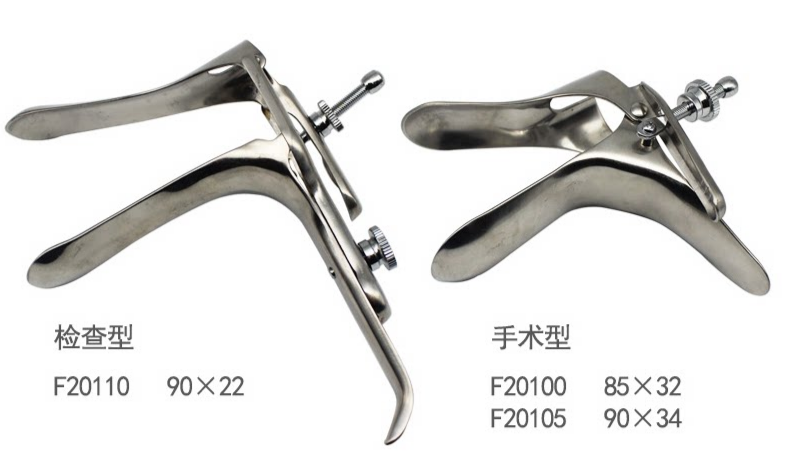
\includegraphics[width=0.5\textwidth]{images/fig_speculum.png}\\
{\footnotesize 图：窥阴器（speculum，俗称"鸭嘴钳"）实物——金属两瓣式，带手柄/旋钮，撑开两瓣即可露出宫颈。妇科 TCT 涂片、HPV 取样、盆腔检查都用它。常见\textbf{金属（不锈钢/钛）}和\textbf{一次性塑料}两种；\textbf{有大有小}（不同口径），\textbf{疼可请医生换小号}。它和 BDSM 语境里夹乳头的"乳夹"是两种东西，只是中文都叫"鸭嘴钳"才容易混。}
\end{center}
\par\smallskip

\noindent\textbf{检查时的真实体验}（提前知道能少一半紧张）：
\begin{itemize}[leftmargin=2em,itemsep=0.3em]
  \item \textbf{冷金属触感}：器械是冷的，插进去的第一感是"凉"——\textbf{这是正常的，不是痛}。
  \item \textbf{撑开的胀感}：两瓣张开后会\textbf{撑住阴道壁}，有\textbf{胀、满、被顶住}的感觉——\textbf{不是"撕裂"}，是"撑开"。
  \item \textbf{取样时的"刮"感}：TCT 用\textbf{小刷子}在宫颈上转一圈，HPV 用\textbf{棉签}刮取——\textbf{有轻微异物感}，\textbf{不是"疼"}（除非有炎症/宫颈脆弱）。
  \item \textbf{全程 30 秒--2 分钟}：熟练医生很快，\textbf{别"越检查越害怕"}——\textbf{越紧张阴道越紧}，反而更不舒服。
  \item \textbf{检查后可能有少量血丝}：\textbf{1--2 天}内出现\textbf{少量褐色分泌物}属正常（取样时蹭到宫颈微血管），\textbf{超过 3 天或量多}就医。
\end{itemize}

\noindent\textbf{怎么让自己舒服一些}：
\begin{itemize}[leftmargin=2em,itemsep=0.3em]
  \item \textbf{放松}：吸气时放松、呼气时让医生操作——\textbf{别"憋气用力"}（肌肉绷住反而更紧）。
  \item \textbf{提前说"怕疼"}：医生会\textbf{换小号窥阴器}或\textbf{操作更慢}，\textbf{不用硬撑}。
  \item \textbf{憋尿别太满}：太满会顶住、不舒服；\textbf{稍微有点尿意}反而好（膀胱充盈让宫颈位置更"正"，医生更好操作）。
  \item \textbf{经期别查}：经血影响涂片结果；\textbf{最佳时间：月经干净后 3--7 天}（宫颈最"干净"、取样最准）。
  \item \textbf{前一晚别性生活}：精液/润滑剂会影响涂片；\textbf{也别用阴道栓剂/冲洗}。
\end{itemize}

\noindent\textbf{一句话总结}：鸭嘴钳 = \textbf{妇科检查器械}（撑开阴道看宫颈用），\textbf{冷 + 胀 + 刮}是正常触感；\textbf{放松 + 提前说怕疼 + 经期别查}——记住这三点就够用。

\section{性交意外、经期性生活}（来自旧书"女性在性交中的意外与经期/孕期"，已用现代观点改写）

\textbf{性交中的意外}：
\begin{itemize}[leftmargin=2em,itemsep=0.3em]
  \item \textbf{阴道痉挛（dyspareunia/vaginismus）}：性交前阴道括约肌强烈收缩、难以插入，多与\textbf{恐惧、疼痛史、创伤}有关；处理核心是\textbf{放松 + 渐进训练（阴道扩张器）+ 必要时性治疗}，不必"猛泼冷水"。
  \item \textbf{性交后头晕/意识丧失}：可能与心血管/神经有关，剧烈或过度紧张时可出现；\textbf{面色苍白、大汗、血压低、晕厥要平卧休息，不缓解就医}。
  \item \textbf{组织薄弱期避免剧烈}：经期、产后恶露未尽、哺乳期、炎症、术后、绝经后阴道壁弹性差，\textbf{过剧可致撕裂、出血}——用润滑、放慢、避开脆弱期。
\end{itemize}

\textbf{经期性生活}：
\begin{itemize}[leftmargin=2em,itemsep=0.3em]
  \item 经期\textbf{不是禁忌，但需防护}——经血是细菌良好培养基，\textbf{全程安全套 + 注意清洁}可大幅降低感染风险。
  \item 部分女性经前/经期性欲反而增强，属正常个体差异；\textbf{不舒服就停}，不勉强。
  \item 经期行经量增加、经血逆流理论上略增，\textbf{经痛明显者不建议经期行经}。
\end{itemize}

\textbf{孕期性生活}：详见本册《孕期性生活专题》章（D 补充）——核心是\textbf{孕早期（尤其有流产史）谨慎、中晚期侧卧/后入位、避免压迫腹部、破水/前置胎盘/出血时暂停}。

\chapter{不孕不育治疗}


病史


1．一般情况：职业性质，工种，是否高温作业，有无接触工业毒物如铅、汞、磷等。有无接触放射线，防护措施如何。有无过量烟酒嗜好，营养状况，精神状态等。

2．以往是否患过性病、腮腺炎、结核病、附睾炎、前列腺炎、膀胱炎、肾盂肾炎、脊髓损伤等。是否患有重症糖尿病、肾脏病、甲状腺机能减退等。

3．妻子健康状况、职业等。性生活情况。

4．双方化验检查情况，女方妇科不孕症检查情况。

5．家族中有无不育症患者、两性畸形患者、遗传病患者及结核病、精神病、传染病患者等。母亲在怀孕期间有无流产、死胎等。





认识病因


精液异常

（1）无精子或精子过少。无精子可为永久性或暂时性。永久性见于先天性睾丸发育障碍或睾丸、输精管严重病变；暂时性多见于性生活过频，精子减少。多次检查精液，精子密度低于0.6亿／毫升，女方受孕机会减少。低于0.2亿／毫升时，常造成不育。

（2）精子质量差。精液中无活力的或死的精子超过20％～25％，或精子活动能力。

（3）睾丸局部病变。如睾丸结核、附睾炎、睾丸肿瘤、腮腺炎并发睾丸炎、精索静脉曲张等均可致不育。

影响精子与卵子结合的因素

（1）附睾、输精管、射精管、尿道等任何一处病变均可阻碍精子的运行而造成不育。（2）逆行射精。（3）外生殖器官畸形。

内分泌障碍

脑垂体机能减退，先天性肾上腺皮质增生，睾丸发育不全、原发性或继发性腺功能低下、甲状腺机能减退等亦可造成不育。

其他病因

某些全身性疾病、重症营养不良、经常接触放射线、高温作业、药物中毒性影响、长期服用粗制棉籽油及精子免疫抗体的存在、精液中果糖缺乏、前列腺素异常等，均会导致不育。

环境污染

20世纪以来，精子浓度和精子计数发生长期下降，睾丸异常的发生率有了显著增加。反映男子生育力全面下降。人类男性精液的平均精子密度已由1940年的1.13亿／毫升下降到1990年的6600万／毫升，每次射精的平均精液体积由3.40毫升下降到2.75毫升。环境污染是造成这一变化的根本因素。特别是疾病、营养不良、社会经济状况、长期慢性紧张、情感压抑、嗜烟、酗酒、药瘾和职业性有毒害物质如重金属、杀虫剂、麻醉剂、细胞生长繁殖抑制剂、抗代谢药物和辐射等环境因素都会对生殖健康造成影响。





常规生化检查


生殖器官的检查

包括对阴茎、尿道、睾丸、附睾、精索、前列腺等器官的视诊、触诊等。查看阴茎是否为严重包茎，有无硬结炎症、肿瘤、发育异常等。尿道排尿困难、瘘孔、下裂、硬结及狭窄。对前列腺检查其大小，有无肥大、硬结、肿物，取前列腺液送实验室检查。测量睾丸的大小、硬度，有无硬结、压痛、鞘膜积液、肿物，是否为隐睾。输精管的硬度，有无结节、压痛以及有无精索静脉曲张等。

睾丸体积的检查常用以下方法：

（1）卡尺测量法。此法所测结果较准确，但比较繁琐。方法为用卡尺分别测量睾丸的长径、宽径、厚径；然后用各种公式计算出睾丸体积。

（2）测量子比较法。睾丸体积测量子为不同体积的状如睾丸的椭圆形硬物，依其大小标为1～25号。测量时将被测睾丸拉起，绷紧阴囊皮肤，将测量子于睾丸旁逐一与之比较，与睾丸大小最相近的测量子体积，即可视为睾丸体积。

正常男子睾丸体积的个体变异很大，左右两侧的两个睾丸亦有一定差异，因而所测结果只能作为参考。对睾丸发育状况以及生殖能力的估计须经多方面检查加以综合分析，才能得出结论。

据调查，正常成年男子的睾丸体积（包括阴囊皮肤在内）大多相当于15至25号测量子的体积。

精液检查

是男性不育的必查项目。检查包括精液量、颜色、粘稠度、酸碱度：液化情况、精子密度、活力、形态等。

（1）颜色。正常人精液颜色是灰白色，禁欲时间长精液呈浅黄色。若精液呈乳白色或略带黄绿色，常是由于生殖道或副性腺感染，精液中含有白细胞之故，精液发红或夹有血丝血凝块，称血性精液。

（2）精液量。正常健康男子，每次性交射出的精液量为1.5～6毫升，精液体积异常一是过少，少于1毫升；二是过多，超过8毫升。精浆是精子的营养来源，其中含有稳定精液酸碱度的缓冲物，能保护精子在酸性阴道分泌物内的存活。精子只占精液量的1％，精液体积异常一般是精浆成分出现变化。如果精液量过少，精浆不能稀释精子，精子往往失去活力，从而造成不育；精液过多时，精子密度降低，精液过稀，易于从阴道内流失，不利于受孕。

排精量不足1毫升或只有二三滴时，称之为精液量过少。性交次数过于频繁时，精液可以显著减少，可禁欲5～7天重新测定。如果取精不得当，使精液失去，也可能造成精液量过少。造成精液量过少的原因还有：

1.附性腺因素：包括睾丸功能障碍；附性腺出现感染或其他病变时。

2.射精管梗阻：可因尿道狭窄、尿道憩室引起，也可能因感染水肿造成。

3.膀胱括约肌功能紊乱，或局部神经支配失调时，可出现部分性逆行射精。

精液量过多可见于精囊炎，当炎症分泌物过多时，精囊液显著增加。大多数原因不明的少精子症患者，可采用分段射精和离心分离精子的方法取精，将精液离心浓缩精子后进行人工授精。

如果患者睾丸发育不良、射精管道完全阻塞、不射精、逆行射精时则根本无精液排出。

（3）酸碱度。正常酸碱度为pH7.2～8.0。过高或过低都可影响精子的活动和代谢。若超过8.5，常说明精囊有炎症，或精液放得时间过久。若低于7，则是射精管阻塞，也可能是精液被尿污染。

（4）液化。精液刚射出时是粘稠的液体，但因受精囊分泌的凝固酶的作用很差，或畸形精子超过30％，常可造成不育。

（5）精液理化性状异常。正常精液射出后很快凝成胶冻状，在以后的15～30分钟内又全部液化。如果精液射出后不凝固，或液化不全，过稠或脓性分泌物使精子活力下降，造成生育能力低下。生殖道感染也可引起不育。精液中致病菌大于103个／毫升，非致病菌大于103个／毫升，均可引起不育。

生精障碍

（1）性染色体异常可使睾丸等性器官分化不良，造成真假两性畸形以及生精障碍；常染色体异常可导致性腺及生精细胞代谢紊乱。造成不育。

（2）隐睾症或双侧睾丸发育不全者无生精能力。单侧睾丸功能正常者，仍可生育。

快凝结成胶冻状，继而在15～30分钟内又因前列腺分泌的液化酶而恢复成液状。这种过程称为精液液化。若超过30分钟还不液化，即为不正常。精液不液化，精子不能自由活动，当然也就不会生育。精液不液化的原因，大多是由于前列腺的液化功能障碍所致。

精液粘度和液化时间是精液正常与异常的重要指标之一，主要取决于男性生殖腺中蛋白溶解酶的活性。无论精液粘稠度增高或降低，都可改变精子在精液中的活动能力。精液粘度和液化时间的异常与生殖道炎症、酒精中毒、酶原疾病等有关。

精液电描记图是测定精液粘度和液化时间的一种方法。把精液置于装有凝固描记仪的空气恒温器内检测，记录精液液化的电描记图，判断精液的粘度和液化时间。精液电描记图测定排除了主观因素和环境因素的影响，整个过程由电子描记显示图形，较为准确可靠，可用于诊断因精液物性质障碍有关的男性不育症和观察治疗效果。

（3）精子数量。精子的数量一是指每毫升精液中的精子数；二是指一次射出的精液中的总精子数。精子数量的个体差异很大，与其年龄、健康状况以及近日是否有过射精有关。检查前应禁欲3～10天。一般成人每毫升精液中精子数量为2000万～1.5亿／毫升。要反复检查多次。一般认为，如果多次检查精子数量均低于2000万／毫升，应视为精子过少。这类患者即使精子形态、活力等均正常，生育能力亦较常人低，甚至造成不育。大于2.5亿／毫升者称为精子过多症。

精子数量减少的原因，可因睾丸本身发育障碍、外界环境因素、内分泌疾病等原因所致。精子密度过高也会影响精子的活动，发生流产的机会也比较多。有些人虽然精子密度低于2000万／毫升，但精子活动力强，畸形率低，依然能生育；有些人尽管精子数量并不少。但活动精子百分率低，畸形精子多，结果也不能生育。一般认为，精子计数的最低限度，密度是1000万／毫升；每次排出精子总数是5000万。低于这个标准，基本上无生育力。

（4）精子活力：一般取已液化的精液一滴，在显微镜下观察，并计数，大约计算出活动与不活动精子的百分率。一般可将精子的活动力分为五级：

1级精子毫无活动，全部为死精子。

2级精子原地打转，动作迟钝。

3级精子能活动，但不活泼，缓慢向前游动，方向不呈直线。

4级精子以中等速度直线向前游动。

5级精子活泼，快速直线向前游动。

精子活力包括精子活率和精子活动力。

精子爬高试验是测定精子活动速度的一项试验，是判断男子生育力的一项指标。取塑料管灌满含有果糖的精液营养液，管的上端结扎。下端垂直插入含有少量精液的试管内。放入37℃恒温水浴箱中8小时，取出，将塑料管剪成1厘米长12段，依次把每段精液溶化后滴于计数盘上作精子计数，计算精子上升的高度及数字，以判断精子活力。

此法简单易行。对测定精子运动速度、判断生育能力有一定的价值。

（5）存活率。通常在射精后1小时内，能活动的精子至少占70％，若少于50％则为不正常。输精管道及附属性腺的炎症、精液标本放置在过热或过冷的环境中、盛放精液容器中的影响、长期禁欲、精子受免疫影响而导致精子凝集等原因可致精子活动能力及存活率减弱。

（6）精子形态。形态正常的精子不应少于85％以上。如畸形精子在10％以下时，对生育无显著影响；在20％以下时，仍有生育可能，若超过20％则可能造成不育。

精子分头、体、尾三部分，正常精子长约50～60微米，外形如蝌蚪状。头部正面为卵圆形，前面是扁平的，侧面是梨状的。前缘锐薄，尾部长而弯曲，能作摇摆状活动，于液体中以每秒25微米的速度向前移动。正常精子头部可以变异为大头、小头、圆头及尖头等不同形态。幼稚型精子可呈小头状，可见头部胞质残余及体部胞质残余等。衰老的精子在头部胞浆内可见深染颗粒、头部深染或不着色等。

1.头部：精子头长3.5～5.0微米，宽2.0～3.0微米；精子头呈规则椭圆形。只要精子其他形态正常。精子头大小不是重要因素。精子头部异常包括：圆锥形（长宽分别小于5和2微米，或长超过5微米，宽小于3微米）、不规则形、双头和“梨形”。

2.中段：中段长5.0～7.0微米，宽1.0微米。宽超过2微米多反映胞浆小滴未完全退化，如果胞浆小滴大于精子头的一半，意味着精子不成熟，属异常，若小于或等于头的一半应属正常。中段断裂也属异常。

3.尾部：尾长45微米。尾部异常常见为断裂、双尾或卷曲。卷曲可能与锌元素含量有关。其他缺陷可能与无症状生殖系统感染有关。

一个精子可能有多种缺陷，可以按其主要缺陷统计。精子形态判断时应包括以下内容。

＞60％的正常椭圆形精子头（包括半数左右的可疑者），若＜30％不正常；

＜6％的圆锥形精子头，若超过10％不正常；

＜8.6％的不规则精子头。若超过50％不正常；

＜0.5％的不成熟精子，增多意味着精子生成或精子成熟过程出现障碍；

＜20％中段缺陷，若超过25％不正常；

＞20％尾部畸形，若超过25％不正常。

如果形态异常的精子超过70％，特别是妻子有习惯性流产时，男方很可能具有染色体异常。如果异常精子少于70％，也许是精索静脉曲张、职业或环境接触毒物、放射线、微波、服用药物、感染及应激等因素影响了睾丸生精过程。精子形态异常时，因为头过大或其他形态异常不利于穿透宫颈粘液所形成的微小通道。宫颈粘液中常可见到头特别小的精子，多数因为无顶体存在。如果畸形精子症找不出任何明确原因时则为原因不明的睾丸生精障碍，可以采用中医药治疗方法促进生精。

精液异常的原因有：

（1）睾丸疾患：

（1）有隐睾病史者，无精子症发生率显著升高，即使有精子，精液质量也异常。

2.睾丸损伤，伴有阴囊血肿或血尿，无精子症或精液异常发生率显著增加。

3.曾发生过睾丸扭转可有无精子症和少精子症。

4.睾丸炎和附睾炎的病人，其精子密度和活动率显著降低。

（2）泌尿生殖道疾病：

（1）性传播疾病一般不影响精子密度。但精子活动率下降。

2.泌尿生殖系统炎症常使异常精液质量，精子形态和活动率较低。

（3）其他系统疾病：

（1）青春期前后发生腮腺炎可引起无精子症，精液异常。

（2）支气管炎特别是支气管扩张无精子症发生率显著增高。气管炎患者的精液分析异常率增高；

3.糖尿病与射精功能障碍相关，但不引起精液质量异常。

4.6个月内曾发高烧的可使精液异常率明显升高。

（4）其他：

1.长期服用对生育产生影响的药物。无精子率显著升高，如各种细胞毒及抗肿瘤药物、某些磺胺药等。

2.高温工作中缺乏适当劳动保护条件，产棉区长期食用未经处理的棉籽油。常见到睾丸萎缩、少精子、死精子或无精子症患者。

3．体外异种受精实验：常规精液分析的各项指标完全正常，有时也不一定能使精子具有受精能力。目前常用人精子穿透仓鼠卵子的异种受精实验。验证男性不育者的实际生育能力。

精子穿透仓鼠卵试验是根据仓鼠卵去除透明带后，几乎不再具有种属特异性的特点而设计的，用人精子穿入仓鼠卵的百分率来评价精子的受精能力。

一般从4～12周龄的雌性仓鼠获取卵子，经处理放入含有一定数量已获能精子，在370c温度中孵育3～5小时，然后吸出卵子在显微镜下观察。凡卵子卵浆内有肿大的精子、头并附有尾部者认为已受精，并且计数。

这种方法是诊断男性不育症一种很有实用价值的方法。

精子宫颈粘液穿透试验是：

（1）玻片法：使精子与宫颈粘液直接接触，试验不能真实地反映客观情况，并难以标准化及定量。

（2）毛细管法：将粘液放入一端封闭的毛细管中，另一端直立浸在粘液中，观察精子群的活动能力。

精子穿透宫颈粘液能力与精子活动力的大小有关。宫颈粘液有筛选形态异常精子的能力，不合格的精子不能穿透宫颈粘液。如果精子在试验中穿透能力正常，常提示不孕是由女方宫颈粘液异常所致。

前列腺液检查

正常前列腺液为白色，呈微酸性，pH6.3～6.5。内含总脂28.6毫克％，其中磷脂占65％。白细胞数在10个以内，并可见到少许上皮细胞、淀粉样物体及精子。患前列腺炎时，镜检白细胞数增加，或见成堆的脓细胞，卵磷脂颗粒减少。

内分泌检查

目前常用的方法有：血浆睾酮水平测定；人体绒毛膜促性腺激素刺激试验；促性腺激素释放激素刺激试验。

克罗米芬是合成的女性激素衍生物，此药可诱发排卵和产生精子，临床常用于治疗少精子症。应用克罗米芬以后能增强丘脑下部促性腺激素释放激素的分泌，睾丸分泌睾酮也因而增加。所以克罗米芬刺激试验，是检查丘脑下部功能的良好办法。

试验需时12天，在服克罗米芬之前，先查两天血浆和黄体生成素的基础水平。从第三天开始连续服克罗米芬10天，用量为200毫克／日，一次或分次口服。在服药后第九、十两天测定血浆睾酮和黄体生成索的浓度。正常用此药10天后与对照值相比较，黄体生成素的增长幅度为72％～24.5％，卵泡刺激素为45％～130％，睾酮为40％～22.0％。从增长幅度可以看出。卵泡刺激素增长幅度不如黄体生成素及睾酮明显，因此阳性指标是以黄体生成素及睾酮的增长幅度为主。青春期前儿童的刺激试验反应为阴性时，提示青春期尚未开始，但不能预示是否开始发育。16岁时一般呈阳性反应，若年龄超过17岁，兴奋反应不明显，则应进行垂体功能检查。在青春期少年或青春期后成年，若克罗米芬刺激试验是阴性，那么，一般来说，年龄越大，则垂体功能低下的可能性越大。成年男性病人患单纯垂体性幼稚症，可以本试验阴性作为诊断参考。至于原发性睾丸功能低下病人，一般是黄体生成素值偏高，用药兴奋后不再上升。原发性无精子或精子稀少的病人，本试验呈阳性。

人体绒毛膜促性腺激素刺激试验人体绒毛膜促性腺激素（HCG）是由胎盘分泌的激素。HCG能促进男性胎儿的睾丸分泌少量睾酮，对男性胎儿的副性器官发育有意义。虽然在妊娠终未HCG已降至很低水平，但已成熟的睾丸已能分泌睾酮，足以使睾丸正常下降。HCG也能促进女性卵巢分泌雌激素和排卵，临床上常用此药治疗不育症。为男病人进行HCG刺激试验，可检查体内的睾丸组织是否具有分泌功能。检查结果如为阳性，表明体内睾丸组织有分泌功能。如检查结果反应偏低，应考虑为隐睾症或原发性睾丸功能低下。如为阴性反应，也不能立即作出相反的诊断。女性病人检查HCG的变化，目的在于诊断早期妊娠、葡萄胎及绒毛膜上皮癌等疾病。

促性腺激素释放激素刺激试验。在下丘脑的神经分泌物中，含有促性腺激素释放素（GnRH）。若GnRH神经元损伤或垂体功能低下时，睾酮的分泌会有明显减少。GnRH刺激试验的目的，在于检查垂体的功能。

血浆睾酮水平测定血浆中睾酮的浓度个体差异很大。正常壮年期男性（20～50岁）的水平最高，平均约为570～7009微克％，50岁以后，其浓度逐渐减少。血浆睾酮的水平在昼夜间有差异，早晨8～10时最高，午夜2时最低。睾酮分泌过多，原因可为睾丸的良性问质细胞瘤，血浆睾酮比正常人多100倍，因而表现为肌肉和骨骼的生长过快，性器官过早发育和副性征过早出现。睾酮分泌不足，可见于因手术、感染、化学中毒、放射线损伤或发育不全等原因而致睾丸功能低下。也可能继发于垂体病变，因促性腺激素减少。以致睾丸间质细胞发育不良。目前测定血浆中睾酮含量的方法很多。如放射免疫法，由于血浆用量较少，误差也少，有一定优越性。

睾丸活组织检查

男性能否生育首先检查睾丸组织是否受到过损害，生精功能是否正常。进行睾丸活组织检查，除诊断男性不育外，还可诊断睾丸其他疾病。睾丸活组织检查有两种方法。

（1）穿刺法。用针管及针头，抽吸少许睾丸组织。

（2）切开法。阴囊皮肤作2厘米左右的小切口，剪下一小块睾丸组织。

睾丸组织切片检查时可见，在正常情况下，青春期前曲细精管细小，无基底膜，仅有原始生殖细胞和支持细胞，间质细胞不明显。青春期后则表现为曲细精管直径加宽，有较薄的基底膜。上皮细胞能显示精子发育成熟的各个时期。精原细胞靠近基底膜，成熟的生殖细胞靠近白细胞管管腔，管腔内可有较多精子。睾丸的生殖病理变化，主要出现在曲细精管生精上皮和曲细精管基底膜。

男性不育症经睾丸活动组织检查，一般常见的病变如下：睾丸不成熟，其组织为青春期前的组织；精子发生低下，各时期精子都有，但数量减少；曲细精管变性，曲细精管透明变性或纤维化；克氏综合症，可见曲细精管细小，无生精细胞，唯有支持细胞的基底膜增厚，有时表现为透明；单纯支持细胞综合症，无各期生殖细胞，仅有支持细胞：成熟障碍或生精阻滞生精过程被阻止在初级精母细胞或精原细胞阶段；睾丸组织接近正常，不育的原因应考虑输精管道被阻塞。

总之，睾丸活组织检查，是确诊男性不育症的重要方法。

输精管、精囊造影常用于男性不育症的检查

通过尿道或阴囊部注入造影响剂，使射精管、精囊、输精管及附睾显影，以了解各部输送通道梗阻、炎症、结核、先天性畸形及其临近组织的有关病变。

常用的输精管、精囊造影方法有下述两种。

（1）经输精管法。切开阴囊外上部，显露输精管，用注射针刺入输精管注入造影剂1.5～5毫升。

（2）经尿道逆行插管法。先用尿道镜或膀胱镜插入尿道后，在精阜两旁找到射精管开口，将细导管插入1～3厘米，然后注入造影剂2～5毫升。

输精管、精囊造影对于诊断男性不育的原因有着重要意义，可以发现精子运输通道的先天性畸形、炎症、肿瘤等疾病，另外对前列腺病变的诊断也有一定的帮助。

多普勒超声检查

对可疑的精索静脉曲张及隐性精索静脉曲张患者，通过一般物理检查不易确诊时用多普勒超声仪检查能获得较为准确的结果。

免疫学检查

目前最常用的抗精子抗体测定技术有精子凝集试验、毛细血管内凝集试验、胎盘内凝集试验、补体依赖性精子制动试验以及抗体标记荧光免疫技术等。

精子凝集试验的血清精子凝集抗体滴度取1:32作为有临床意义的低限标准。低于1:32者生育力稍有减低。1:64～1:512为中滴度，可以生育，但生育力较低，1:512以上为高滴度，表明被检者无生育力。精浆中的抗精子抗体滴度与血清中的滴度也不完全一致。精浆的精子凝集抗体滴度1:16，生育力显著降低。但并不是不能生育；滴度高于1:32，可能不育。这些滴度数值只适用于精子计数每毫升2000万以上的男性不育患者。

汉光免疫法检测，不管其他方法检测抗精子抗体是否阳性，它总是约有30％的患者出现阳性反应。所以，临床上价值不大。

混合抗球蛋白反应试验，此法特异性较强。测定抗精子抗体的准确性超过90％。由于操作技术简单，可作为一种筛选试验。

染色体检查

染色体异常者一般生育功能都受到影响。如果一个不育患者的睾丸体积小于12毫升，或者两性畸形都应该检查染色体，因其染色体异常的可能性很大。另外，妻子有习惯性流产或畸胎史时，夫妻双方应做染色体鉴定。

染色体异常有两种情况：一种是染色体的数目异常；另一种是染色体的结构畸变。

在男性不育中，性染色体数异常引起的病症常见的是先天性曲细精管发育不全综合症，其典型核型是47XXY，还有47XXY/46XY嵌合型。在女性不育中，性染色体异常的疾病有性腺发育不全。而染色体结构畸变中，染色体易位是引起不育症的一个主要的原因。如果夫妇有一方是染色体平衡易位携带者，虽然他本身并无异常表现，但可能给后代带来染色体异常的危险性。这样的胚胎在妊娠早期流产的可能性很大，幸存者可能是染色体病患者。因而在妊娠20周左右应做产前诊断，通过羊水细胞培养鉴定胎儿的染色体的结构和数目是否正常，异常时应及早做人工流产。

检查染色体一般是从患者静脉采血1.5毫升，鉴定核型和分辩染色体的数H和形态结构。染色体检查为遗传疾病以及某些其他疾病的病因、发病机制、诊断、预防以至预后等提供了科学依据。

交媾试验：交媾试验是检查精子是否能穿过宫颈的试验方法。

精子射进阴道后要穿过宫颈。宫颈粘液由宫颈腺体分泌。宫颈粘液的量和性质随月经周期中雌激素和孕激素水平出现周期性变化。在月经中期，宫颈粘液大且稀薄、拉丝长，使精子易穿过。如果精子活动能力差，或宫颈粘液少而粘稠，或存在抗精子抗体等，将会影响精子穿透宫颈粘液。

（1）试验的时间：在月经周期中，宫颈粘液能够允许精子穿透的时间的长度每个妇女不同。同一个妇女的每个周期也有差异。应因人而异确定出进行精子穿透试验的最佳时间。可采用B超监测排卵来判断排卵日期。试验应该尽可能靠近排卵期进行，可以根据基础体温、宫颈粘液的变化和阴道细胞学检查来确定排卵时间。

每对夫妇在进行试验前应该至少禁欲2天。在同房前24小时内禁止阴道内用药或冲洗。上床前把大小便排尽，避免同房后几小时内上厕所。性交后仰卧，屈膝，垫高臀部休息至少30分钟，防止精液流出。试验应在性交后6～8小时进行，18～24小时进行也是可以的。

（2）性交后试验技术：医生将没有涂抹滑润剂的阴道窥器插入阴道，用不带针头的注射器、吸管，分别吸取阴道后穹窿、宫颈外口和宫颈内口的宫颈粘液，高倍显微镜下观察精子情况。

1.阴道后穹窿样本。由于阴道内酸性环境，精子在阴道内仅能存活2小时，检查阴道样本的目的在于证实精液确实进入阴道内。

2.宫颈外口样本。宫颈外口精子数目随着性交后时间延长而减少。性交后2～3小时，在宫颈下段积聚大量的精子。在宫颈粘液中，根据精子移动情况可以分为4级：1．迅速和直线向前运动；2．缓慢直线或非直线运动；3．非向前运动；4．不活动精子。

一对正常夫妇性交后，在宫颈内样本通常用400倍视野可以观察到25个以I级和II级活动精子，如果用高视野有10个以上I级活动精子，即可以认为是良好的；如果仅有5个活动精子，并且为迟钝缓慢或转圈运动形式，则说明精液中精子数目少和活动率差，或者宫颈粘液异常。

性交后4小时开始，宫颈外口的精子数目逐渐减少。所以在4小时以上间隔时间检查，从宫颈下段收集到的宫颈粘液中仅可发现很少的精子。

3.宫颈内口样本。在射精后，少数精子迅速到达宫颈内口，而且数目逐渐增多。约在2～3小时后达到一个高峰。在24小时之内，精子数目相对稳定。

所以在性交后6～10小时，用高倍视野具有I和II级活动度的精子数目大多为10个，即属于正常范围。在性交后10～24小时，可检测到的精子数目与6～10小时相似。

（3）试验结果：性交后试验的目的，不仅在于检查性交后数小时以后，在宫颈粘液中活动的精子数目，而且还要评价精子的活动状况。在性交后6～10小时宫颈内存在适当数量的活动精子，就可排除由宫颈因素引起的不育。

试验阴性不能轻易下结论，因为有可能选择的时间不当。有时由于性交后试验进行得太早或太晚，可以造成假阴性结果。如果不能利用准确可靠的时间来确定排卵时间，则有必要在一个周期中重复作几次性交后试验。

一旦证实性交后试验为阴性，可以进一步确定是精子质量问题，或是由于宫颈粘液的有害因素，并且可测定宫颈粘液中是否存在抗精子抗体。对于性交后试验阴性的不育夫妇，可以利用人工授精办法，帮助他们受孕。





无精子症治疗


【病因】

无精子症占到男性不育症的19％～30％。无精子症可以分为三类：睾丸前性、睾丸性和睾丸后性。

1．睾丸前性：睾丸前性指睾丸本身功能正常，但是由于下丘脑和垂体内分泌功能紊乱而继发引起睾丸不发育或不生精。

2．睾丸性：睾丸性指睾丸本身因各种原因导致其丧失产生精子的能力。最常见的有克氏综合症、隐睾等。产棉区长期食用生棉籽油是无精子症的最常见的原因。继发于腮腺炎的双侧严重睾丸炎是散发性无精子症的原因之一。

3．睾丸后性。睾丸后性指精子运输管道梗阻或先天性缺如，如附睾结核、双侧附睾炎、双侧输精管合并精囊缺如、射精管梗塞等。

【无精子症诊断】

1．测量睾丸体积，一般中国正常成年人的睾丸体积为12～25毫升。睾丸体积小于10毫升者，一般伴有生精功能障碍。

2．测定血中促卵泡激素（FSH）对诊断无精子症具有十分重要的意义。

3．睾丸活检。睾丸生精功能可以分为：严重和不可逆性生精障碍，轻度和中度生精障碍，生精功能较好，生精功能正常或基本正常。

4．果糖测定可以用来鉴别是否存在输精管堵塞问题。

5．输精管精囊造影法可确定输精管梗阻部位。

【治疗】

对于睾丸前性的即下丘脑和（或）垂体功能障碍引起的睾丸功能低下，可以用激素替代疗法。对于睾丸性无精子症，只有那些FSH没有升高的病人才有治疗的希望。如果FSH已明显升高，或者睾丸活检证实为严重和不可逆生精障碍者，可选择人工授精、收养孩子或不要孩子。对于睾丸后性无精症，实行外科手术。

【食疗】

苡仁赤豆粥。苡仁60克，赤豆60克。粳米250克，煮粥服食，日1次。

米粥油。粥锅内滚起沫，浓滑如膏者，就是粥油。每日早晨服1碗。

二鞭膏。牛鞭、羊鞭、猪髓适量，煮烂熬成膏，每服1匙，每日3次。





特发性少精子症


【病因】

特发性少精子症是指那些找不到明显病因而精子计数小于2000万／毫升或每次射精的精子总数小于5000万的不育症，患者无臆睾、睾丸炎、前列腺炎或精索静脉曲张，性功能正常，丸体积大于10毫升。附睾和精索无异常，第二性征正常，无全身性疾病。实际上，精子计数为500～2000万／毫升的男性结婚3年，妻子受孕累积率仍可在50％。

【治疗】

1．克罗米芬治疗法：它主要针对因促性腺激素缺乏而引起的特发性少精子症。精索静脉曲张手术后6个月精子质量仍未改善时也可服用。服用期间出现抑郁、头昏、视力模糊、过敏性皮炎症状时应停止服用。严重肝病患者禁服。

2．低剂量睾酮治疗法：补充外源性睾酮可能对生精功能促进作用。3个月后如果发现精子数目减少或男性乳房增生就要停药。

3．反跳法：大剂量的睾酮抑制生精后停药，即反跳疗法。这种治疗法方应慎重使用，只有那些经其他方法久治不愈的少精病人才可使用。

4．绒毛膜促性腺激素（HCG）治疗法：可以促进睾丸间质细胞生成睾酮，增强生精功能。

5．溴隐亭治疗法：溴隐亭是一种抑制泌乳素分泌的特效药。

6．硫酸锌治疗法：成年男性因缺锌使垂体的促性腺激素减少，引起性功能减退，睾丸缩小，精子生成异常，因此不能生育。

另外，缺锌会使前列腺液中酶系统功能异常，影响精液的液化。还会使精子运动和穿透卵子透明带的能力下降。

最后在饭后服用，以免对胃有刺激作用。平时注意多食用一些富含锌的食品，如肝、蛋、鱼、肉等动物食品，以及花生、核桃等植物性食物。





精液过少治疗


正常的男性，每次排出的精液量为2～6毫升，1.5毫升以下为异常。一般将每次排出的精液量少于2毫升者，称为精液过少。精液过少精液中碱性分泌物不足以稀释阴道中的酸性分泌物。会影响精子的活力；另外，精液过少不能形成足够的精液池，不利于精子进入子宫。

【病因】

1．房事过频或排精间隔期过短，致使精液的产生和存贮不足而引起精液过少；亦可见于精神紧张。

2．全身性慢性疾病如结核病、营养不良等患者，或生殖系统局部病变如前列腺炎和精囊炎患者，尤其是结核性炎症。均可造成精液过少，甚至无精液排出。

【治疗】

对于精液过少的治疗，一般生理性精液过少，只要延长排精间隔期（通常每周房事1～2次），即可使精液增多：精神紧张引起的精液过少，在消除紧张因素后即可恢复；病理性精液过少，应针对不同病因积极治疗全身性或局部性的各种疾病，不论何种原因引起的精液过少，在治疗中均要注意增强体质。

精液精子少的夫妻按摩：

（1）仰卧位。先在以下穴位按揉：关元、足三里、三阴交、太溪穴、关元穴重点按揉约2分钟，至出现较强的酸胀感，并向前阴扩散。足三里和三阴交两穴，两侧均同时按揉，各约1分钟。按揉大溪穴先左后右，共约3分钟，以酸胀痛感为度。

（2）仰卧位。以手掌贴附在病人小腹部，做顺时针方向的环旋摩揉，动作稍慢。直到小腹有温热感为止。再将两手掌根贴在患者两侧少腹部上，顺着少腹部向下推至阴茎根部力量逐渐加重，有一种压发胀感．推30次。

（3）仰卧位。用双手掌抱住其阴囊，相对搓揉约2分钟，力量先轻后稍重，以病人能够耐受为准。再在大腿内侧用掌擦法操作，以透热力度。

（4）俯卧位。将食指屈曲的指间关节突起部，点按在病人腰部肾俞穴，逐渐用力，攘压揉动至出现酸胀感约1分钟。再在腰眼穴用两拳面击打2分钟。然后斜擦骶部八骼穴部位，以透热力度。

【食疗方法】

生山药、白糖各150克，胡椒粉少许，糯米粉250克。山药去皮蒸熟加白糖胡椒粉压泥调馅，包成汤圆食用。适于精子少者食用。





精液不液化


精液在生殖道内是液体状态。从阴茎口射出后，立即变成胶冻状或凝结块样乳白色物质，此时精子无法自由游动，5～45分钟之后，精液自动液化，凝胶变为稀薄的液体。这一过程是酶催化的过程。

开始时呈液态是便于精液的射出。随后形成凝块使精子得到充分休息和获能。一旦液化，精子就有足够的能量穿透宫颈粘液，最终到达输卵管。

精液射出体外，在30分钟内不凝固或液化不全，则为精液不液化。精液液化与精液中所含的酶系统有关。精液液化是与前列腺分泌的纤维蛋白溶解酶的作用有关。因此，精囊和前列腺疾病是引起精液不液化的主要原因。炎症可影响酶的分泌，同时对所分泌的酶还有不同程度的破坏作用，从而导致酶系统失调。促成精液不凝固或液化不全。精液不液化影响精子的生存和活力；不利于精子的输送。

【治疗】

治疗精液不液化应积极治疗原发病，同时可用淀粉酶液化精液：

1．性交前淀粉酶栓剂阴道置人法。药栓在性交前置入阴道内。

2．性交后淀粉酶溶液阴道注入法。在排卵期性交射精后立即注入阴道中。

3．中医治疗：

（1）肾阴亏损证：本证多系素体肾阴亏损，虚火炎盛。精液受灼而出现的以精液粘稠不液化为主症的症候，常伴耳鸣，腰酸膝软，五心烦热，盗汗，口咽干燥等症。成方常选用知柏地黄丸、大补阴丸。

（2）肾阳不足证：本证多系肾阳虚弱，精宫寒冷，气化失常所出现的以精液粘稠不液化为主症的症候，常伴见阳痿早泄，腰膝酸软，畏寒肢冷等症。成方常选用金医肾气丸，五子衍宗丸。

（3）湿热下注证：此证多系湿热下注，扰乱精室，精浊混淆引起的以精液粘稠不液化为主症的症候，常伴见小便灼热，频数淋漓，黄赤混浊，甚则尿血，尿痛等症。成方常选用龙胆泻肝丸加知柏地黄丸，或加六味地黄丸，或加五子衍宗丸。

精液不液化症方用：生牡蛎30克，银花18克，麦冬、丹参各15克，生地黄、玄参、浙贝母、枸杞、仙灵脾各12克，丹皮、地骨皮、赤白芍、枣皮、连翘、夏枯草、柴胡、竹叶、茯苓各9克，水煎，每日二剂，服3天停药1天，24剂为1疗程。多在1～2疗程见效。此证偏阳虚者亦常见，可于上方去银花、连翘、地骨皮、竹叶、夏枯草之类，酌加杜仲、菟丝子、补骨脂、女贞子、巴戟天、附子、黄芪、锁阳、鹿角胶之类。

【食疗】

鲜胎盘1具、鲜羊肾1对，花椒、生姜、食盐一齐放砂锅内文火煮熟，吃肉喝汤。

麻雀蛋2个，白皮鸡蛋2个，乌龟蛋2个，枸杞子50克，肉桂5克。将蛋煮熟去壳，放入砂锅。加入枸杞、肉桂、煮30分钟，加红糖，每日晨服。

100克海参煮汤，加调料同服。

山药炖百合，鲜山药250克，百合25克，加水炖烂，放冰糖10克，分3次服食。

\chapter{不孕不育的中医与食疗（参考）}

本章为旧书整理的\textbf{中医与食疗参考}内容（多为男性不育方的针灸取穴与食疗汤粥酒方），核心思路（补肾、益精、调气血）作为\textbf{辅助参考}保留，\textbf{不替代现代生殖医学诊断与辅助生殖技术}。具体用药/用方须\textbf{辨证施治、遵医嘱}，切勿照方抓药。

\section{针灸取穴（参考）}

（1）无精子症：取穴肾俞、命门、腰阳关、三阴交。两组交替使用，隔天一次，采用补针加直接灸五壮。

（2）精子减少、阳痿不举：用针灸温补肾俞、气海、太溪，以滋摄精，佐命门、腰阳关，以温补肾阳，刺足三里调理下焦。并加服六味地黄丸和五子衍宗丸。

（3）精少、阳痿、不育症：取穴关元、中极、三阴交为主，配以肾俞、命门等穴。操作法：对精神紧张、情绪苦闷的患者，采用强刺激手法，重捻针，留针10～15分钟。患者若有房事过度或长期手淫情况。则采用中等刺激手法，捻针略轻，留计10～15分钟。身体衰弱、烟酒过度、长期脑力、体力疲劳的患者，针法要轻，留针约15～20分钟。针前要排空小便，治疗过程中禁忌酒、咖啡、茶、葱、蒜等刺激性食物。

（4）精液异常：

1.取穴：常用穴：大赫，曲骨，三阴交，中极。关元或八骨，肾俞，命门。

2.治法：每次取一组，隔日交替轮用。第1组，先针大赫。曲骨，三阴交，得气后，施轻刺激补法。留针。即在关元、中极两穴行隔姜灸，灸3壮，艾炷大小以灸区出现红晕力度；第2组先针八骨，得气后，灸肾俞，命门，亦为3壮。留针15～20分钟，留针期间，每隔5～10分钟运针1次。15次为1疗程，未愈者停针5～7天后，继续下一疗程。

针灸关元、中极，使针感向下放射，再刺太溪、照海。均用平补平泻手法，得气后留针，并温针灸各2～3壮。针后取会阴穴，艾条温灸与按摩交替进行约30分钟。隔日1次，治疗20次，休息6日。





\section{食疗汤粥酒方（参考）}


【鳖肉银耳汤】

鳖1只，银耳15克，盐、姜适量。将鳖宰杀制净、切块，银耳水与鳖肉炖熟后加盐调味。食鳖肉，银耳并饮汤。每日1剂，连用5～7天。

功效：滋阴降火。适用于精液不液化所致的不育症。

【双冬女贞子虫草汤】

天门冬、麦冬、女贞子各10克，冬虫夏草15克，蜂蜜30毫升。将上四味水煎取汁，加蜂蜜调服。温服。每日1剂，连用数剂。

功效：滋阴降火。适用于精液不液化所致的不育症。

【参芪雀卵汤】

人参15克，黄芪20克，山药25克，麻雀卵5个。将诸药水煎、去渣。打入麻雀卵搅匀再煮片刻温服。食雀卵，饮汤，每日1剂，连服数日。

功效：健脾补肾。适用于精子活动力差所致的不育症。

【鹿鞭巴戟天汤】

鹿鞭1对，巴戟天、淫羊藿各15克。将上三味共煮至鹿鞭烂熟、切碎。食鹿鞭并饮汤。每日1剂，连服数日。

功效：补肾气，健脾胃。适用于精子活动力差所致的不育症。

【肾绒汤】

鸡肾、鸭肾各10个，猫耳朵30个，猪骨头浓汤1碗，火腿丝10克，淀粉、生姜末、葱白末、胡椒末、食盐各适量。

1.把鸡肾、鸭肾洗干净，放入锅内，用沸水烫一下，随即捞出，把外膜轻轻撕去，剁碎，用面粉和匀，做成30个猫耳朵（食量大者可酌情增加）。

2.将锅放中火上，倒入煮好的骨头汤烧沸，先下猫耳朵，煮熟之后，放入胡椒末、食盐、火腿丝，调匀后煮约15分钟，随即放入淀粉、浓缩原汁，使成绒汤，盛入碗里，撒上生姜末、葱白末，调匀即可。随意分次服用。

功效：补肾助阳。适用于肾阳虚之阳痿、不育症等，或先天性发育不良。

【生精汤】

巴戟、菟丝子各15克。肉桂、肉苁蓉各10克，狗鞭20克，羊肉100克，花椒、生姜、料酒、味精、猪油、细盐各适量。将巴戟、菟丝子、肉苁蓉装入纱布袋内，扎好口，备用。将狗鞭用清水发胀、洗净，用油砂炒酥，再用温水浸泡半小时，与洗净的羊肉同放沸水锅内，于水沸后相继放入花椒。生姜、料酒、肉桂后，改用小火煨至七成熟时，把药袋放入锅内继续炖；待狗鞭、羊肉酥烂后挤出，装碗里，加味精、盐。猪油调好味即可。吃肉，喝汤。

功效：壮阳补肾。可辅治不育症（精子成活率低）。

【生精汤】

熟地、山药、覆盆子、枸杞子、菟丝子各15克，枣皮10克，泽泻12克。将上七味同入砂锅，加水适量煎汤。饮汤。每日2次，早、晚分服。

功效：益肾生精。适用于精液异常、肾精亏所致的不育症。

【狗脊狗肉汤】

狗脊、金樱子、枸杞子各15克，瘦狗肉200克。将狗肉洗净切块，同狗脊、金樱子、枸杞子一起下锅，加水适量，炖40分钟即可。食肉，饮汤。

功效：补肾壮阳。可辅治不育症，常服效佳。

【羊腰汤】

羊肾（腰子）1对，肉苁蓉12克，熟地、枸杞子各10克，巴戟天8克。将羊腰子洗净，切了，与肉苁蓉、枸杞子、巴戟天同入锅，加水适量炖60分钟至腰子熟烂即可。吃肉，饮汤。每日1次。

功效：壮阳补肾。可辅治不育症。

【液化汤】

鳖1只，知母、黄柏、天冬、女贞子各10克，银耳15克，生姜、葱、味精各适量。将知母、黄柏、天冬、女贞子装入纱布袋内，扎口备用；用开水把鳖烫死，揭掉鳖甲，洗净，放入锅内，加适量水及姜片、葱段。先用武火烧开，再改文火煨至肉将熟时，放入水发好的银耳及药袋，待鳖肉酥烂时出锅，加味精即成。

功效滋阴清热泻相火。可辅治不育症（精液不化）。

【益气健精汤】

人参、水发香菇各15克，山药、黄芪各20克，麻雀头5个，母鸡1只，调料适量。将鸡及麻雀头去毛洗净，同入锅内，加适量水上火煮，待七成熟时，加黄芪山药、香菇、葱、姜、盐、料酒后，改温火煨至烂。人参用开水泡开，上笼蒸半小时。饮汤，吃肉，嚼食人参。

功效：健脾胃，补肾气。适用于脾肾气虚之精子活动力差者。

【鹿鞭苁蓉粥】

鹿鞭1对，肉苁蓉100克，米100克。将鹿鞭去膜，洗净切细；肉苁蓉酒浸1夜，刮去皱皮，切细。米洗净，加水煮粥，粥将熟时，下入鹿鞭、肉苁蓉，以及适量葱白、花椒、盐、味精等调味食用。佐餐，连服数日。

功效：补肾壮阳。可辅助治疗不育症。

【食盐拌粥油】

大米250克，食盐适量。将大米洗净，放锅内加水适量。煮粥，至粥将好时。撇出粥油（指煮粥至滚锅时，粥面上出现的米沫）1碗；另将食盐炒过，取适量对入粥油中。每日三次。

功效：补虚益肾。可辅治男子精清不育。

【核槐枸杞粥】

核桃仁50克，枸杞子15克，大米适量。将核桃仁捣碎，大米淘净，加枸杞子、核桃粉和水适量，煮成粥。每日1次，常服。

功效：滋阴补肾。可辅治不育。

【多子酒方】

枸杞子、桂圆肉、核桃肉、白米糖各250克。好烧酒7000毫升，糯米酒500毫升。将上药共装细纱布袋内，扎口，放入坛内，用好烧酒。糯米酒浸泡，封口，窖3周取出。每日2次，每次饮服50～100毫升。

功效：补肾健脾，养血脉，抗衰老。适用于脾肾两虚、面色萎黄、精神萎靡、腰膝酸软、阳痿早泄、精少不育等症。

【围精酒】

枸杞子60克，当归30克，熟地90克，好酒1500克。将上药加工碎，盛入绢袋，置于瓷制容器或其他适宜容器中，加酒封固。每日摇动数下，经14天后开封，取出药袋，澄清药液即成。每日早、晚各1次，每次饮服3小盅，不可过量。

功效：滋阴补血。适用于肝肾精血不足所致的男子不育、头晕腰酸等症。

【鹿龄集酒】

人参、熟地各15克，海马、鹿茸各10克，肉苁蓉20克，白酒1000毫升。将人参、鹿茸研为粗末，再与其他药物一起用白酒密闭浸泡1个月。即可饮用。每日早、晚各1次，每次饮服10毫升。

功效：益气补血，补肾壮阳。适用于气虚及肾阳虚出现的腰膝酸软、性功能衰退、耳鸣，或由于肾阳虚而致的男性不育症。此方能明显地提高机体的体液免疫和细胞免疫功能，并且对骨髓造血的功能有一定的促进作用。感冒发热、高血压等患者忌服。

【公鸡殖酒】

鲜公鸡殖（鸡睾丸）200克，夜交藤、仙茅、路路通、桂圆肉各100克，白酒（50度）2500毫升。上药与酒共置于容器内。密封浸泡30日后即可用。但鲜公鸡殖不宜用水洗或放置时间过长，亦忌日晒。最好是掏出公鸡殖后即投入酒内。每日服3次，早（空腹）、午各服20毫升，睡前服40毫升，60天为1个疗程。

功效：补肾强精。适用于男性不育症。

【雄蚕蛾酒】

雄蚕蛾20只，白酒20克，有条件者选活雄蚕蛾，在热锅上焙干。研末备用。每日早、晚各1次，每次空腹时用白酒冲服雄蚕蛾3克，连服半月以上。或将雄蚕蛾油炸后，平时随意食用。

功效：兴阳助性，益精液，活精虫。适用于肾虚阳痿、早泄、滑精、男性不育、精液量少、精虫活者少等症。

【山药汤圆】

生山药150克煮熟去皮，加白糖150克，胡椒粉少许，调匀成泥。糯米粉250克，调成面团，包成汤圆，煮熟食用。

【羊膏粥】

羊脊骨1骨剁碎，肉苁蓉30克、菟丝子3克以纱布包扎，加水适量，共煮4小时，汤与大米煮粥，可加调料。

【法制黑豆】

黑豆500克泡发，熟地黄、山茱萸、茯苓、补骨脂、菟丝子、早莲草、黑芝麻、当归、桑葚、五味子、枸杞子、地骨皮各10克，加水适量煎煮，每半小时取煎液1次，加水再煎，共取煎液4次，合并煎液，放在大锅中，加入黑豆和食盐100克，以小火煨炖至药液涸干，停火。将黑豆曝晒至干，装罐贮藏，食用有补肾益精功效。

【米酒炒海虾】

食物功效：米酒味甘辛性温，能通阳活血，有兴奋作用。海虾（对虾或龙虾）吐甘咸性温，能补肾壮阳。米酒炒海虾有补肾壮阳，强筋健骨的功效。常用以治阳痿、不育。

【阳起石牛肾粥】

食物功效：阳起石味成性温，入肾经，能温补肾阳。牛肾味甘性平，入肾经，能补肾气，益精髓，除湿痹。阳起石牛肾粥，有补肾壮阳功效。可用于治疗肾虚阳痿。阴囊冷，婚久不育等症。

用法：用牛肾一个，洗净切成小块，阳起石30克，先将阳起石用三层纱布包裹，加水约2500毫升，煎1小时，取澄清液，然后加入牛肾及大米约50克，煮粥。加油盐及葱白调味服食。

【杜仲炙猪肚】

食物功效：杜仲味甘，微辛，性温，入肝、肾经，有补肝肾。强筋骨。安胎的功效。猪肚味甘性温，人胃经，有健脾胃，补虚损的功效。杜仲煲猪肚，有补肾健脾，益精血，强筋骨的功效，可用以治疗肾虚遗精、腰痛、精液量少等症。

用法：杜仲30～50克，猪肚约200克，洗净切成小块。加水适量煲汤，调味服食。

【锁阳煲粥】

食物功效：锁阳味甘性温，入肝、肾经，有补肾壮阳益精，养血强筋，润燥滑肠的功效。锁阳煲粥，有补肾润肠的功效，可用于治疗肾虚阳痿、遗精、早泄、不育、老年气弱、阴虚大便燥结等症。

用法：锁阳15～20克，大米及清水适量，煮粥服食。

【肉苁蓉煲羊肾】

食物功效：肉苁蓉味甘酸成，性温，入肾、大肠经，有补肾益精的功能。羊肾味甘性温，有补肾气，益精髓的功能。肉苁蓉堡羊肾有补肾、益精、壮阳功效，常用于治肾虚精冷、阳痿、腰腿酸软，耳聋便秘等疾患。

用法：肉苁蓉15.30克，羊肾一对，煲汤调味服食。

【枸杞叶煲猪腰】

食物功效：枸杞叶味苦、性凉，入心、肾、肺、脾经，有补虚益精，清热止渴的功能。猪腰，味咸性平，入肾经，有治肾虚腰痛，遗精盗汗的功效。枸杞叶煲猪腰，有补肾益精的功效，可用以治疗精虫数少，存活率低，活动力差，遗精，耳鸣耳聋等症。

用法：枸杞叶100～150克，猪腰一对，洗净切成小块，加水煲汤。调味服食。





不育症的外用药


适用于死精过多

当归、苦参、蛇床子、知母、黄柏各20克，红花、甘草各10克。煎汤薰洗会阴部，或直接坐浴。每晚1次。

适应于脾肾阳虚之精子缺乏症

附子（炮）、肉桂、白芷各9克，淫羊藿、透骨草、大青盐各10克，丹皮5克，赤芍6克，加水煮10分钟，趁热熏洗下腹部及会阴部，再用毛巾浸泡药液，擦洗中极、关元、神阙穴。每日1次。

治疗不育症

苦参、蛇床子各30克，龙胆草、黄柏、土茯苓、泽泻各20克。水煎取药汁，先熏外阴部，后坐浴20～30分钟。

适应于精子缺乏症

睡前宽松衣裤，仰卧床上，两手搓热后用右手顺时针揉丹田100次，逆时针揉100次。每晚1次。

适应于阳虚火衰精子缺乏症

将适量食盐在铁锅炒热，温度适中，放入脐窝，压暖水袋，食盐不热后取出，再做一遍。

适应于精子缺乏症

王不留行粳9克，研末后加黄酒调湿敷脐，外用纱布和胶布盖粘，每天换药1次，20天1疗程，一般5～7疗程。





不孕的检查与诊断


1．一般检查：血常规、尿常规、梅毒血清检查。

2．白带检查：滴虫、霉菌、淋球菌、支原体及衣原体检查。

3．阴道脱落细胞检查：检测卵巢功能、预测排卵期及了解体内雌激素水平。

4．宫颈粘液检查：宫颈粘液评分、同房后试验、体外精子穿透试验。

5．血清学检查：抽血时间要严格按规定日期。

6．子宫内膜活组织检查：在经前2～3天进行，时能提供分泌良好的子宫内膜，判断有无排卵、腺体分泌程度、有无炎症及新生物。

7．X线检查：（1）头颅蝶鞍摄片：了解垂体病变，对月经稀发、泌乳、催乳素增高的病人应作头颅蝶鞍摄片，以排除垂体肿瘤。（2）子宫输卵管造影：以明确宫腔有无畸形、粘连、结核、炎症等；宫颈内口是否松弛；输卵管是否通畅。（3）盆腔充气造影：肥胖妇女或未婚者疑有盆腔病变而双合诊或肛腹诊不能查明者；疑有生殖器官发育不全或畸形者；明确多囊性卵巢、功能性卵巢肿瘤、卵巢萎缩等，盆腔充气造影，可以辅助临床检查的不足。

8．免疫学检查：（1）抗精子抗体。通过精子制动实验和精子凝集试验检查。（2）透明带自身抗体。明带自身抗体测定有助于诊断。（3）体液免疫反应。试验，补体依赖试验；免疫荧光法；酶标记免疫法（酶联免疫吸附测定法；放射免疫分析法，免疫吸附测定法等）。（4）细胞免疫反应。白细胞移动试验；白细胞粘附抑制试验；淋巴细胞转化试验；外周白细胞促凝血活性测定；花环试验。（5）精浆免疫抑制物测定。抗补体法；单向免疫扩散法；间接免疫荧光定位等。（6）抗卵子抗体检查。（7）抗子宫内膜抗体：免疫金银法；间接免疫荧光法；EIA法；EISA法；PHA法；琼脂双相免疫扩散法等。

9．细胞染色体检查：包括性染色质检查，染色体检查。可诊断常染色体显性遗传疾病、常染色体隐性遗传病、x性连锁隐性遗传病、x性连锁显性遗传病、妇科病的染色体核型。

10．排卵监测：测基础体温间接反映卵巢功能。宫颈粘液检查也能反映体内卵巢内分泌功能变化。

11．阴道涂片：观察和了解各种激素的阴道脱落细胞的单独作用，为临床上分析和评价各种片型所反映患者的内在内分泌环境。

12．B超可检查卵泡发育情况。

13．腹腔镜检查。

14．腹腔液：排卵后经腹腔镜可吸到15～25毫升的腹腔液，由于卵泡破裂释放卵泡液，此时腹腔液中黄体酮及雌二醇的浓度较卵泡期明显增高。

15．子宫内膜活检：子宫内膜对卵巢激素有很高的敏感性，雌、孕激素的失调可以从内膜变化中反应出来。内膜检查是一个迅速、安全、可靠及廉价的诊断方法。可检查卵泡发育不良、雌激素分泌不足引起的内膜变化；无排卵的子宫内膜变化、子宫内膜增生过长的情况、黄体障碍引起的内膜变化、卵巢卵泡期不正常内膜的分泌形态以及性激素的过度分泌。





不孕的治疗


先天性发育异常

1．外阴闭锁：完全性闭锁较为罕见。多为表浅性闭锁。可手术治疗。

2．处女膜异常：处女膜闭锁是女性生殖器官发育异常中较常见的。当发生阴道粘液经血潴留时，处女膜鼓起。在初潮前发现以切开为好。

3．阴道横隔：阴道横隔可完全或部分阻挡阴道。在儿童期可导致大量阴道粘液潴留，至青春期则成隐性月经。

4．阴道闭锁：阴道闭锁者的阴蒂、阴唇、尿道常正常。处女膜环微内陷。

5．卵巢发育异常：包括卵巢下移异常、性腺发育不全、先天性卵巢发育不全。

6．真两性畸形：具有卵巢和睾丸两种性腺组织。真两性畸形中性腺以卵睾为多见。诊断必须通过开腹探查或腹腔镜从外观辨认出卵巢与睾丸两种组织，并对性腺进行活检。送病理检查，明确两种组织的存在。不能只靠外生殖器和性染色体作出判断。

生殖系炎症

外阴各部的急慢性炎症，阴道先天畸形，阴道口疤痕性狭窄或会阴修补缝合过紧、宫颈癌手术后阴道过短、滴虫性阴道炎、霉菌性阴道炎、阴道萎缩、宫颈肥大、宫颈过长、盆腔炎症、子宫内膜异位症病灶等，因为通道狭窄或阻塞，性交疼痛反射性阴道痉挛，阴道口湿润度不足等。炎症治愈后，有些人能很快受孕。

引起不孕的常见疾病

1．黄体功能不全：有很多不孕症和反复流产是黄体功能不全造成的。它是最常见而轻微的卵巢功能异常。

2．黄素化未破裂卵泡综合症：为临床表现不明显的病症。在不明原因不孕症的发病率很高。

3．多囊卵巢综合症：多囊卵巢综合症涉及下丘脑、垂体、卵巢、肾上腺、胰腺及遗传等诸多因素。

症状：为月经稀发、闭经、不孕、多毛、肥胖，偶有排卵，但大多数无排卵，基础体温单相，月经第一天子宫内膜呈增殖期变化，只有一半的患者中有典型临床表现，25％则除不孕外无其他症状。

4．高催乳素血症：各种原因所致外周血中催乳素浓度异常增高为高催乳素血症。哺乳、应急、服药、胸壁刺激等因素可引起高催乳素血症。

一般治疗

1．加强锻炼，增强体质，注意营养，有利于不孕症患者恢复生育能力；掌握性知识，学会预测排卵等受孕知识，增进受孕机会；忌用烟酒，消除不良的精神因素，调节心态，保持心理健康。

2．病因治疗：器质性疾病，如发现肿瘤、处女膜闭锁，瘢痕粘连、阴道横隔；滴虫、霉菌感染或其他炎症应积极治疗；宫颈管狭窄、粘连者，可单纯扩张宫颈即起到治疗作用；子宫发育不良。可针对病因，服用激素或子宫内放置小型节育环2～3个月；宫腔粘连，可进行扩张官腔及分离粘连术。

3．诱发排卵：诱发排卵药物包括氯米芬，绝经期促性腺激素，黄体生成激素释放激素，溴隐亭，绒毛膜促性腺激素。氯米芬为首选药物，用促排卵药过程中需观察宫颈粘液、血雌激素水平，B超监测卵泡发育。

4．促进或补充黄体分泌功能：对黄体分泌功能不足补充黄体酮。

5．改善宫颈粘液：月经周期第5天给雌激素10天。

6．输卵管阻塞的治疗：输卵管近端阻塞可采用输卵管内注射药液，可在官腔镜下输卵管内注药效果更佳。输卵管远端阻塞可行输卵管造口术，根据不同情况可选择输卵管整形术，输卵管结节切除和吻合术，输卵管宫角吻合术，输卵管官腔内移植术。

7．免疫性不孕的治疗：避免接触抗原，官腔内人工授精，免疫抑制剂。

人工授精

结婚后三年左右，尚未生育者，经过医院作详细检查和多方治疗后仍无效，证明确实不能通过性交受孕时，可以用人工授精的科学方法以达到受孕生育的目的。人工授精不是通过性交方式而是用人工的方法（用注射器注入的方式）。把精液输入女方的生殖器使精子和卵子结合而受孕生育。

精液可以是自己丈夫的，也可以用自愿供精者的精液。前者称配偶间人工授精，后者称供者人工授精。供精者的精液和自己丈夫的精液混合进行人工授精，称混精人工授精。

人工授精用的精液可以是新鲜的，也可以用低温冷藏的冷冻精液。新鲜精液和冷冻贮藏的精液受孕率，都在65％以上。冷藏精液可贮存在精子库，随用随取，不用因等待排卵期授精反复采取精液，一个供精者的精液可以冷藏起来，需要时可提供给一个或若干个妇女进行多次人工授精。这样也有利于对接受授精者的保密。精子冷冻到零下196℃仍可以存活。

丈夫人工授精的指征是女方经过检查认为确实有受孕生育能力，男方的精液经过化验符合标准，但是由于男女的生殖器官有畸形，如男性尿道下裂、阴茎严重屈曲畸形、阴茎海绵体硬结症、阳痿、早泄、逆行射精；女方的阴道狭窄、阴道痉挛、阴道内疤痕粘连、外阴道口畸形、阴道过度松弛存贮不住精液，以及子宫颈狭窄、子宫位置明显前屈或后倾等，从而影响性交或精液不能正常地射入阴道内者。

供者人工授精的指征是经过检查确认男方属于绝对不育症。比如无精子症、严重少精症（每毫升精液中含500万精子）。精液有如下的异常，如精子计数每毫升在2000万以下；精液量减少在0.5毫升以下的精液过少症；精子活力低弱，畸形精子多，精液排出后持续凝固而液化不全等造成不育，可以采用供者人工授精。男方患有精神病或者其他严重的遗传性疾病。虽然男方有生育能力，但禁止用这类患者的精子受孕，也可采用供者人工授精的方法生育。此外，若夫妇双方由于免疫不相容因素造成不育以及有遗传性疾病的家族中的近亲结婚。也可采用供者人工授精。接受供者的精液受孕生育，要牵涉到一些复杂问题甚至法律问题。所以，应当慎重考虑，与有关医疗和司法单位共同商讨，事前办好规定的一切手续。

对适合做供者人工授精的夫妇，医院应负责为他们严格地选择供精者：

（1）调查并保证供精者家族中有无遗传性疾病与近亲结婚史。

（2）个人应无烟酒嗜好，生来无重要病史，年龄在25～35岁之间，具有中等以上文化水平，智力与人格发育正常，五官端正。身材适中，健康无病。

（3）已婚，爱人亦无吸烟嗜好，家庭和睦，性生活正常，已有发育正常的子女。夫妇双方的工作场所不接触有害射线与有毒物质。

（4）供精者应与接受授精者（受精者）的丈夫同一民族。在身材、皮肤颜色以及面貌等也尽量与受精者的丈夫相接近为好。供精者的血型与受精者相适合，最好与其丈夫同血型。

（5）供精者的精液，在精子数量、质量方面要超过正常水平。

（6）医务人员必须严格保密，供精者与受精者夫妇之间无任何联系，绝对不准向外传播这方面的任何情况。

供精者采取精液是以手淫法自行收集。性交中断法、阴道外排精法等，均不如手淫法方便。为了保证供精者的精液能够达到人工授精的精液标准，采取精液前一周，应无性交、手淫或遗精。人工授精的精液标准是：精液量4～6毫升，精子计数6000万／毫升以上，活动率80％以上，明显畸形精子少于20％。接受人工授精者要经过三个月以上的基础体温测定并配合连续性的宫颈粘液结晶及阴道细胞检查，明确其排卵期，人工授精最适宜的时机是宫颈粘液分泌最多的排卵前期。因为卵子从卵巢排出后生存时间仅8～24小时，精子在女性生殖道里最多存活48小时，精子从女方阴道游动到输卵管与卵子相遇平均约需12小时。所以，准确地测定排卵日期是很重要的。用最近三次月经周期的平均天数减去14天为排卵日也可以。在家庭里利用测量基础体温的方法，就是把“低温相”向“高温相”转换日之前，体温最低日或者“低温相”最后的一天推断为排卵日。每个月经周期进行三次人工授精，就是从排卵日前三天开始，每隔一天做一次人工授精。如月经周期28天的人，在月经的第11、13、15天。月经周期30天的人，在月经的第13、15、17天各做一次。若具体地按小时算是，在排卵日期前72小时、24小时和排卵后24小时。若未成功，可以再重复地测准排卵日期，继续人工授精几个月经周期。必要时，可以用药物诱导和调整好排卵期来提高受孕率。以手淫法采集精液时，用温水、肥皂把手和阴茎洗净擦干，把精液射到干燥灭菌或煮沸消毒过的大口瓶里，保持在37℃以下，在1小时内用于人工授精，受精者仰卧在妇科检查床上，取膀胱截石位，常规外阴消毒，用消毒窥阴器充分暴露子宫颈，阴道和宫颈周围也要常规消毒。把1～2毫升精液吸到带细塑料管的无菌干燥的注射器里，把塑料管插进子宫颈管里0.5～1厘米，慢慢地注入精液0.5～1毫升，把多余的精液注到阴道后穹窿处。还可以把精液直接注射到子宫口处，形成精液池，使精液漫过子宫颈的外口。如果阴道的酸性度偏高，可以先用碳酸氢钠等碱性液体或葡萄糖盐水等冲洗阴道，有利于精子活动。还可以利用子宫帽或者小塑料杯，精液注入后，把子宫帽套在宫颈上，或者把盛有精液的小塑料杯放在宫颈外口，使之紧贴宫颈。这些方法都可避免精子接触阴道内的酸性分泌物。上述方法的主要目的是让精液和宫颈外口直接接触，有利于精子进入子宫腔里。过去把精液直接注入子宫腔里，容易引起痉挛性疼痛、出血或者感染。

施行人工授精后，把臀部抬高，仰卧休息30～60分钟，有利于精子进入官腔。为了预防感染，人工授精后应服用抗生素两天，禁止性生活2～3天。受精者回家后可以正常活动和工作。在人工授精后，受精者应连续测定基础体温和到医院检查宫颈粘液结晶和阴道细胞学变化。如果基础体温的“高温相”持续20天以上，则表示有受孕的可能。虽有“高温相”同时还有阴道出血或小腹不适，应注意预防流产。

人工授精后的受孕率可达65％以上。由于冷藏精液人工授精技术的不断提高，冷藏精液与新鲜精液的受孕率相接近。人工授精受孕后自然流产的发生率与正常妊娠者相同，甚至还低些。人工授精生育的子女发生先天性缺陷者比正常性交受孕生育的子女少得多。供者人工授精后生育的男孩多于女孩。但开展供者人工授精技术需要有一套严格的医疗制度和法律手续。

“试管婴儿”

“试管婴儿”的全称是体外受精和胚胎移植，主要适应证是输卵管不通、宫颈粘液阻碍精子穿透、子宫内膜异位症和精子数量和活动率低于正常者。这种方法不是每种类型的不育症都适合。做“试管婴儿”手术的妇女必须具备正常的卵巢和子宫功能，子宫内膜适合受精卵的植入。妇女年龄一般不要超过40岁。

“试管婴儿”主要过程是：

1．促使卵子成熟：目前常用药物刺激卵泡发育和人为地控制排卵时间。常用促排卵的药物有克罗米芬、人绝经期促性腺激素（HMG）、人绒毛膜促性腺激素（HCG）等。采用这种药物刺激方法可以获得多个卵子。

2．在超声波监测下取卵：取卵的方法各种各样，目前较常用的取卵方式是经阴道取卵。将一个阴道超声探头放进阴道，测量好卵泡的准确位置，用负压装置将卵子吸出。这种取卵方式仅需局麻。病人痛苦少，穿卵准确。在每个病人身上平均每次可取到5个卵子。

3．试管内受精：卵子采集4～8小时后每个卵子与经过筛选的5万到50万高活力精子共同温育12～24小时。如果受精，再继续培养24～48小时。

4．胚胎移植：在卵子取出后30～50个小时，将分裂成2～6个细胞的胚胎经宫颈口植入子宫内，一般植入三个胚。受精卵往往不能在子宫内膜着床。妊娠后流产率较高，40岁以上妇女更易发生流产。多胎妊娠易发生围产期死亡。

配子输卵管内移植术

配子输卵管移植术，简称GIFT，配子是精子和卵子的统称。是将卵子和精子直接注入输卵管让其自然受精，分裂，转移进子宫，植入，而不是体外受精后再人工移植进子宫。GIFT只适用于那些输卵管通畅的妇女，由于输卵管的机械阻塞或疾病不能自然排卵。

向输卵管内注入精子和卵子一般采用腹腔镜技术。GIFT完毕，缝合好手术切口后。让妇女在病床上静卧8小时，即可自由活动了。

试管婴儿的体外授精的成功率是很高的，但胚胎移植的成功率却较低。而GIFT避免了体外授精的胚胎处理、移植的过程，精子和卵子的受精过程是在输卵管内进行的，其后的受精卵转移、分裂和植入过程与自然受孕过程相同，所以GIFT的成功率高于试管婴儿。

中医治疗

中医治疗不孕，先要调经，辨证治疗因肾阳虚、肾阴虚、肝郁、痰湿、血瘀引起的月经不调等证。

1．针灸：

（1）肾虚型：输卵管疾患及子宫内膜疾患。

体针：太溪、石关、大赫、水泉、关元、子宫，均用补法，每日或间日1次，留针30～60分钟，同时温针或灸，10次为一个疗程，连续针3个疗程。

配耳针：肾上腺、子宫、交感、内分泌。

（2）气滞血瘀型：子宫内膜病变及输卵管闭锁或粘连。

体针：蠡沟、带脉、阳陵泉、中极、子宫、气海，均用平补平泻法，太冲穴用泻法，每日或间日1次，留针30分钟，10次为一个疗程，连续针3个疗程。

（3）痰湿内阻型：子宫内膜增殖症，增殖倾向，输卵管梗阻或粘连。

体针：天枢、水道、归来、气冲、关元、子宫，三阴交，均用补法，每日或间日1次。留针30分钟，10次为一个疗程，连续针3个疗程。

2．食疗：

蛋类和鱼子：高蛋白，应多食。蛋类每日1～2个，鸡蛋偏热，鸭蛋偏寒。宫寒不孕者，可多食鸡蛋，黄带、赤带者，可多食鸭蛋。鱼子不宜进食过多。

野味、水产品，如野鸡、野鸭、野兔、鸽子、乌鸡、童子鸡、牛羊猪肉及各种鱼虾、龟鳖之类。鹿肉壮阳；生虾仁浸酒滋阴补肾。

鳗鱼味甘性平。《本草汇言》曰“补肾脏，壮虚赢”，《日华子本草》曰“起阳”。

牛鞭选用带睾丸者洗净、斩段、清水煮沸，弃腥水，再仔细取毛及杂物，用筷子通净尿道内“臊物”。加黄酒500～1000毫升，白酒250毫升，葱姜。加一勺红糖及半杯啤酒，不必加水，烧开后小火炖烂如膏。牛鞭补肾阳、益阳气，可单用或混入中药中，每日50毫升，空腹服用，适用于肾阳不足、肾气亏损、阳痿遗精、腰膝酸软、畏寒肢冷等症。

猪、牛汤骨或小排骨汤：煮前先将汤骨敲碎，煮时加少量米醋，可使骨髓有效成分更多溶入汤内。骨髓有助于造血、生精、改善性功能。

【木耳冰糖羹】

白木耳润肺，黑木耳补肾，黑、白木耳同用，有金水相生之妙用。黑、白木耳比例自定，适量，先煮沸黑木耳，文火煨3小时，加白木耳煮沸后文火煨1小时至烂似细泥，加冰糖适量，备用，每日250m1空腹服用。冬季可适量加入小枣。

【淡菜粥】

淡菜50克，温水浸泡半日，烧开后去心，加糯米100克，煮成粥，放盐少许，每日趁热早晚服两次，治肝肾不足所致的不孕。

【苁蓉羊肉粥】

肉苁蓉15克，羊肉量不拘，加水100毫升，待肉烂后加水300毫升，粳米50克，煮至米开汤稠，再加少许葱姜，再煮片刻，每日早晚温热服食。治肾亏宫寒、肝肾不足所致的不孕。

【生薏苡仁粥】

生薏苡仁洗净，加水，煮酥烂如粥，每日250毫升空腹服用，功能健脾、渗湿。性微寒而不伤胃，益脾而不滋腻，清补利湿。

【素补膏滋】

酌选黑芝麻、核桃肉、津小枣、莲子肉等，用阿胶炼成膏滋，每日50～100毫升空腹服用。补气养血，宜女子服用。用于气血两虚、头晕目眩、失眠、心悸、食欲不振。

3．外敷疗法：

（1）千年健30克、羌活20克、透骨草60克、独活20克、血竭15克、穿香30克、红花30克、没药30克、当归尾30克、赤芍30克、艾叶60克、白芷30克、五加皮30克、川椒15克、川乌20克、土鳖虫30克、防风20克、干漆20克，上药研细末，置于布袋内，蒸透后热敷小腹部或两侧少腹，每日敷1～2次，每次20分钟左右，每包药一般可连使用10～12天。

（2）透骨草30克、香附15克、丹参15克、艾叶9克、鸡血藤30克、皂角15克用布包袋蒸透后热敷小腹部或两侧少腹；或将药加醋适量放铁锅内炒热敷小腹部或两侧少腹；或将内服中药药渣用布外敷于腹部。脐部、或患病处，待药渣变冷后在其上面放置热水袋，以保持药渣温热，使药力通过皮肤而透入体内病患处。也将药渣加醋30克放入铁锅内炒热后，敷小腹部或病患处。

本外敷法多用于子宫内膜异位症、盆腔炎、输卵管阻塞所致腹痛而不孕者。外敷时注意温度不可过高，以免烫伤皮肤。

\chapter{人工流产、引产知识}


什么是人工流产


在妊娠24周以前，采用人工方法，把已经发育但还没有成熟的胚胎从子宫里取出来，结束妊娠的目的，称为人工流产。人工流产按妊娠月份大小可分为早期人工流产和中期引产。妊娠12周到前做人工流产称为早期人工流产；妊娠12～27周做人工流产称为中期引产。





人工流产手术的适用与禁忌症


人工流产是指在妊娠14周前用手术或药物终止妊娠。妊娠14周以内为早期人工流产，14～24周为中期引产。

1．妊娠12周以内要求终止妊娠而无禁忌证者；10周以内最为适宜。

2．因某种疾病不能继续妊娠者。

禁忌证如下：1．各种疾病的急性期；术前测体温两次超过37.5℃者。2．生殖系统炎症，需治疗后再视实际情况决定是否手术。3．全身情况不良不能耐受手术者，经治疗后有好转，可考虑住院手术治疗。





人工流产的分类


常用的早期人工流产手术有吸宫术和钳刮术两种，前者适用于10周以内的妊娠妇女，后者适用于10～14周的妊娠妇女。妊娠10周以内子宫不太大，胎儿和胎盘尚未形成，一般不需要扩张子宫颈，很容易将胎块组织吸出；手术中反应轻，出血少，手术时间短，术后休息1～2小时就可以回家，恢复也很快，对身体影响小。

1．吸宫术按操作又分为两种：

（1）早早孕终止术：适用于妊娠6周以内者，具有出血少、痛苦小等特点。

（2）负压吸引法：是我国目前常采用的手术方法。先应用探针及宫颈扩张器扩大宫颈，采用电动吸引器产生负压，通过吸引管吸净胚胎组织。

2．钳刮术：妊娠10～14周时，因胚胎逐渐长大，胎盘已经形成。子宫也随着长大，这时做人工流产不宜用简单的吸宫术，而需要采用钳刮人工流产。该手术难度大，出血多，恢复也比较慢。对身体有一定影响。

3．引产术：妊娠超过了14周就不能做上述两种人工流产，而需要住院作引产手术。手术种类包括：注射利凡诺、前列腺素、天花粉蛋白以及水囊引产和削宫取胎。这些手术有一定风险，可能增加孕妇的痛苦。





女性流产手术后的注意事项


1．手术后观察：人工流产手术结束后应观察2小时，注意阴道流血和腹痛情况。如果没有什么反应才可以回家。

2．休息：一般术后应适当休息几天。若体温正常，阴道流出的血性分泌物少。无腹痛等不适。可以起床活动，并适当做些轻微的家务劳动。

3．外阴卫生：在人工流产后的一段时间内，子宫内膜上的创伤尚未恢复，子宫颈口松弛，宫颈内原来的粘液已被去掉。新的尚未形成。此时如不注意外阴部卫生，阴道内细菌容易进入官腔引起感染。因此，人工流产后要更加保持外阴部清洁卫生，勤换洗内衣、内裤、月经巾。2周内或阴道流血未净者绝对禁止灌洗阴道及坐浴，以免引起上行性感染，最好洗淋浴。

4．加强营养：流产后应进食鸡蛋、牛奶、排骨、鸡、鱼等高蛋白、易消化的食品；同时多吃一些富含维生素类的食物如蔬菜和水果，以补养身体。不要忌口或偏食。

5．禁欲：1个月内禁止性生活，以防生殖器官感染。

6．治疗感染：如果有发热、腹痛，或阴道分泌物有异常气味，可能为感染所致，要及时就诊。人工流产时胎盘被剥离后，子宫壁上所留下的创面可有少量出血，这种情况随着子宫收缩及创面修复，一般在3～5天后阴道流血渐渐停止。最多不超过10.15天。如果阴道流血量超过月经血量，持续时间过长，这时需要及时就诊治疗。

7．坚持避孕：落实避孕措施，以免再次受孕和多次人流。

8．检查：术后如无异常，一个月后应检查一次。

9．其他：预防着凉和感冒。





手术后常见并发症及防治


人工流产手术操作简单、时间短，按手术常规操作，是很安全可靠的。但确实也有少数孕妇由于多种原因而产生一些并发症，主要有：

1．出血：人工流产手术时出血超过200毫升者称为流产时出血。这大多由于妊娠月份较大，特别是妊娠13～14周时做钳刮手术过程中子宫收缩不好、大块的胎盘组织不能及时取出、子宫及宫颈的损伤等所致。尽量避免大月份的钳刮是减少出血的关键。大月份钳刮手术应由经验丰富的医生进行。

2．人工流产综合症：个别孕妇在手术过程中，特别是在用宫颈扩张器扩张宫颈内口时，突然出现面色苍白、出冷汗、胸闷、血压下降及心律紊乱、心动过缓，严重者可发生抽搐、昏厥等现象，这统称为“人工流产综合症”。轻者，停止手术后很快就恢复正常；重者，可给予氧气，或静脉内注入阿托品1毫克，一般说均能很快恢复正常。

3．流产不全：少数孕妇术后阴道有不规则流血。量多且伴有血块及下腹部疼痛现象。妇科检查发现子宫颈内口松，有时可发现有血块或胎盘组织堵塞于宫颈外口，或B超检查宫腔内有组织残存。这是由于手术残留而造成的流产不全，应在用抗生素控制感染后清理官腔，刮出官腔内容物送病检。

4．感染：受术者术后感到有下腹部疼痛、腰酸、白带多且伴有发热等现象。这是细菌侵入子宫内膜、输卵管等造成急性子宫内膜炎、子宫肌层炎、盆腔结缔组织炎等所致。造成感染的主要原因是无菌操作不严密，术前原有生殖道炎症未能及时发现与治疗。感染一旦发生，应及时使用抗生素以控制感染。

5．子宫穿孔：子宫穿孔往往是由于手术者术前未能很好地查清楚子宫的位置，或由于宫颈内口狭窄粘连、手术者强行将探针送入子宫内造成。一旦疑有子宫穿孔发生，应停止手术，对子宫损伤处进行修补。手术应给予大剂量抗生素以控制感染的发生。

6．羊水栓塞：大多发生在大月份钳刮手术时，孕妇突然感到胸闷、气急、呼吸困难等。体检可发现孕妇颜面及全身青紫、心率变快、脉搏细弱、血压下降等。应暂时停止手术，进行抢救。

7．宫颈管及宫腔粘连：人工流产术后受术者出现周期性下腹部疼痛。经量减少甚至闭经。检查发现子宫增大，B超见官腔内有积液现象，应疑有宫颈管及宫腔粘连的发生。对宫腔粘连者，可进行钝性官腔分离术。如粘连严重。分离困难，不能强行一次分离成功，可先用强的松及抗生素治疗一段时间后，再进行分离手术。术后，应同时在宫腔内放置IUD半年。术后使用抗生素预防感染。





什么是药物流产


药物流产是指在怀孕早期不须手术、而是通过用打针或服药的方法达到人工流产。应用药物使妊娠终止，是近20年来的最新发展。目前常用的药物是米非司酮（Ru486）和前列腺素联合应用，前者使子宫蜕膜变性坏死、宫颈软化，后者使子宫收缩，促使胚胎排出。药物流产简便、有效、无创伤，避免了进宫腔操作可能造成的并发症。





药物流产的适用与禁忌症


目前国内外常用为米非司酮合并前列腺素类药物流产。这适用怀孕49天以内的妇女药物流产，完全流产率90％左右，失败率4％左右，停经天数越短效果越好。但也存在流产后出血时间长，因不全流产引起感染大出血等问题。

适应证：与一般人工流产相同，更适合于孕期8周以内高危妊娠、负压吸引术有困难或有危险而需终止妊娠者，如有多次妊娠或近期人工流产史、剖宫产吏、哺乳期或子宫畸形合并妊娠等。

常见禁忌证如下：

1．禁忌使用米非司酮者：患肾上腺疾病、糖尿病等内分泌疾病、肝肾功能异常、血液和血管栓塞疾病、与甾体激素有关的肿瘤等。

2．禁忌使用前列腺素者：心血管系统疾病、青光眼、胃肠功能紊乱、哮喘、癫痫等。

3．过敏体质。

4．带器妊娠。

5．宫外孕或可疑者。

6．贫血。

7．妊娠剧吐。

8．长期服用抗结核药、抗癫痫药、抗抑郁药、西咪替丁等。

9．每天吸烟超过10支或嗜酒者。





药物流产的操作方法


用药第1天首服米非司酮50毫克，8小时后服25毫克，第2天早晚各服25毫克，第三天上午8时服25毫克后。到医院一次（顿）服米索前列醇3片，每片200微克，或在阴道后穹窿放置卡前列甲酯栓I毫克。观察半天。米索前列醇口服方便且副作用小，已在临床上广泛采用。





药物流产效果


1．完全流产：用药2周内自行排出完整绒毛和胎囊，伴有蜕膜组织或无蜕膜组织。未经刮宫而自然转经；或未见明确的胎囊排出，出血自行终止，B超未见胎囊，且正常转经子宫恢复正常大小。

2．不完全流产：用药后已排出绒毛和胎囊，在随诊过程中，因出血过多或时间过长，或2周血绒毛膜促性腺激素仍未恢复至正常水平，可行诊断性刮宫。刮出物经病理检查有残留绒毛。

3．失败：用药2周内未见妊娠产物排出，B超仍见胎囊或残留物，或引起难免流产，最终采用负压吸引术终止妊娠。





操作药物流产时的注意事项


1．用药前必须通过B超检查排除宫外孕。

2．用药后必须严密观察孕妇，定时测脉搏、血压，有没有胃肠道反应、腹痛、过敏反应和阴道流血等情况。

3．用药后注意保留阴道排出物，以便鉴别有无绒毛胎囊和蜕膜。

4．如有异常情况如体温升高、剧烈腹痛和阴道大量流血等，应立即就近就医。

5．使用药物流产后出血时间超过两周者，应重复测定血或尿的绒毛膜促性腺激素水平，或做B超诊断是否有孕产物残留，以便及时进行诊断性刮宫。手术前使用抗生素以预防感染。

药物流产虽是一种受群众欢迎的非手术终止早孕的方法，但各种药物流产方法的完全流产率明显低于负压吸引人工流产术。且存在着一定的副作用和不完全流产引起大出血的危险。所以，药物流产是为那些妊娠49天以内需要终止妊娠而又不宜做手术的孕妇提供的一种非手术流产的方法。

药物流产应在具有抢救的医院施行。最后一次用药后应留院观察6小时。





中期妊娠引产


中期妊娠引产法是在妇女怀孕14～26周之间人工终止妊娠的方法。妊娠时间越长，可能发生的并发症就越多，越严重。因此，应该严格掌握中期妊娠引产的适应证。为保证孕妇的安全和健康，中期妊娠引产必须在有一定的技术条件和急救设备的医院内进行。

利凡诺引产

利凡诺引产的作用机制是复杂的，这与多种因素有关，其中蜕膜变性坏死、释放前列腺素是终止妊娠的主要因素。前列腺素可引起子宫收缩，宫缩本身又可促使前列腺素的合成和释放，从而使收缩更加强烈而导致流产。

适应证：1．妊娠14～27周，要求终止妊娠、无禁忌证者。2．因某种疾病，如心、肝、肾、血液的疾病和高血压病等，不宜继续妊娠者。3．因某些遗传病或胎儿畸形等需要终止妊娠者。

常见禁忌证如下：1．各种疾病的急性阶段和孕妇全身情况不良者，如各种感染急性期、心力衰竭、严重贫血等。2．生殖器官炎症，如阴道炎、宫颈炎、盆腔炎等。3．腹壁皮肤有感染者。4．子宫体上有手术疤痕者。5．妊娠期反复有阴道流血者。6．手术前测体温两次在37.5℃以上者。

水囊引产的适用与禁忌

放入水囊后机械性刺激作用，促使前列腺素合成与释放而达到引产目的。

妊娠在14～24周之内不能应用依沙吖啶（利凡诺）终止妊娠者；因某种疾病不宜继续妊娠者。

常见禁忌证如下：

子宫有瘢痕者；生殖器炎症，如阴道炎、重度宫颈糜烂、盆腔炎或阴道分泌物异常；严重高血压、心脏病或血液病，各种疾病的急性阶段；妊娠期间反复有阴道出血者；当天2次体温（相隔4小时以上）37.5℃以上者。





高危人工流产术


高危人工流产术是指受术的孕妇患有某些疾病或子宫畸形，或近期曾接受人工流产术等，给此次手术带来困难，甚至出现意外损伤等。因此，凡属高危人工流产术的孕妇应住院施术，必要时应请有关专科医生会诊，以保安全。更主要的是应加强避孕。防止施行高危人工流产。

高危人工流产术的危险性

1．年龄小于20岁或大于50岁者妊娠而要求终止者，应住院并请有经验的医生进行手术。

2．半年内有终止妊娠或1年内有2次人工流产史者，子宫尚未完全恢复，再怀孕后子宫较软，易发生子宫损伤。

3．剖宫产术后或产后1年之内哺乳者，剖宫产术后的子宫壁上有瘢痕，在1年之内子宫壁尚未充分愈合，加上怀孕后子宫壁较薄，手术时极易从瘢痕部位穿孔。为预防穿孔，术前孕妇应到医院咨询，便于采取必要的手术措施，使手术安全进行。

在产后1年内哺乳的妇女怀孕，其子宫壁比较薄、软，在进行人工流产术时，也很容易穿孔。

4．生殖道畸形或有盆腔肿物者应主动告诉医生。以免术后发生阴道出血。

5．子宫位置高度倾曲或暴露宫颈困难者会给手术带来困难，应住院请有经验的医生施术。

6．既往妊娠有胎盘粘连及大出血者此次手术时仍可因胎盘组织与宫壁粘连而致大出血，因此，术前应验好血型及配好血，一旦大出血，立即输血和予以宫缩剂治疗，以保安全。

7．有子宫穿孔或阴道宫颈穿破史者此次手术时，在原来穿孔部位可能再次发生穿孔。因此，术前应做好一切准备，如必要时采用适当的麻醉方式。

8．脊柱、下肢、盆腔病变不能采取膀胱截石卧位者必要时可采用全麻，以便纠正体位，并应由有经验的医生操作，以防发生意外。

9．并发内科严重器质性疾病或有出血性疾病史者应住院施术，必要时请有关科室会诊，使受术者得到妥善处理。

\chapter{避孕药品}


避孕药品安全性


1．是否致癌。长期服用对子宫内膜癌和卵巢上皮性肿瘤有保护作用。对乳腺良性纤维瘤和纤维囊性增生也有保护作用。药物时间越长防护作用越大。

2．是否影响生育。停药后3月内80％恢复排卵，1年内95％～98％恢复排卵，服药后无影响。

3．是否影响后代。停药后短期怀孕并不增加胎儿畸形发生率。

4．对机体代谢的影响。约半数表现糖耐量降低，空腹血糖正常。少数人可能有血清甘油三脂、磷酯，低密度脂蛋白升高，胆固醇一般不变，停药后消失。卒中和心肌梗死的发生率会有所增加，特别在35岁以上吸烟妇女。





女用避孕药服用方法和注意事项


美国化学家Russell Marker发现，北卡罗莱那州的一种薯蓣含有一种植物甾体，它可以缓解月经痛。1942年他又到墨西哥收集了更多的薯蓣根。随后的几年他从这种植物甾体合成了孕激素。即使是今天，墨西哥薯蓣仍然是一种现代口服避孕药中孕激素（地索高诺酮）的来源。1953年George Pincus（“避孕药之父”）及其同事发现，孕激素可以抑制兔子排卵，随后做了妇女的临床试验。后来又发现，加上雌激素成分可以改善月经的规律性。

避孕药40年来的发展的两个主要趋势：1．雌激素剂量的减低。1968年，30％的口服避孕药中雌激素剂量超过50微克，而今天所有最流行的口服避孕药中雌激素剂量不超过35微克。50年代首次用于临床研究的避孕药的雌激素含量为150微克，是现代口服避孕药妈富隆的5倍。2．“选择性”更高的孕激素。新型的孕激素（如去氧孕烯，也叫地索高诺酮）能改善口服避孕药对心血管疾病方面的不良影响。它们高的选择性（同孕激素受体的亲和力高）避免了以往避孕药具有的不良反应。因此，含有现代孕激素的口服避孕药可以改善痤疮，而以往的产品常常增加痤疮。

我国避孕药的研制也已有30年左右的历史。经过医学工作者的不懈努力，解除了许多避孕药物使用上的误区，掌握了一些避孕药物的科学使用方法。

下面简单地介绍一些常用避孕药物的科学用方法及其注意事项。

避孕的一般原理是甾体类避孕药主要是抑制排卵；改变宫颈粘液的粘稠度，阻止精子穿过；改变受精卵在输卵管内的运行速度，使受精卵发育与输卵管运行速度不同步；改变子宫内膜，使之不利于孕卵着床，从而达到避孕目的。目前国内外常用类型为甾体类女用避孕药，是以人工合成的雌激素及孕激素复合制剂为主，也有单方孕激素制剂。可分为短效、长效、速效、缓释系统避孕药和长效避孕针剂五大类。





短效口服避孕药


短效口服避孕药是主要由人工合成的甾体激素制成、大多数是雌激素和孕激素的复合制剂，少数为孕激素的单方制剂。常用短效口服避孕药有：口服避孕片1号、口服避孕片2号、口服避孕片0号、复方18甲基炔诺酮片（滴丸）、复方左旋18甲基炔诺酮片（滴丸）、三相片、妈富隆、敏定偶等。

【优点】

按说明服药，安全，能持续提供避孕效果。

有助于预防子宫癌和卵巢癌。

月经周期有规律。痛经可能缓解。

若有痤疮，有助于改善症状。

若无任何禁忌证，又能每年随访一次，便可一直使用直至更年期。

无性生活异常。

可逆，停药后可恢复生育能力。

【缺点】

经间出血，尤其是服药的头两个月。

恶心呕吐，但通常在第三个月时就会消失。吃饭时或睡前服药可减少上述症状。

乳房肿胀及触痛感。偶尔出现情绪激动或体重增加。

服药妇女需要高度自觉，记住每天按时服药。

在个别情况下，服药者可能发生严重的副作用。

患高血压且年龄大于35岁的吸烟女性服药后增加心脑血管疾患的机会。

长期服用有发生静脉血栓的危险。

与某些药同时服用，可降低避孕效果。

【检查】

1．了解口服避孕药的优缺点，以及可能出现副作用，以及服用方法、注意事项。

2．如出现下列问题时，应建议去看医生：

疼痛——头部（严重或持续头痛）

——胸部

——腹部

——腿部

视力——模糊、重影、部分失明

黄疸——皮肤及眼睛发黄

气短——当休息或轻度活动时

3．服药前可作下列各项体检：血压、体重、尿检、皮肤、四肢、心脏、乳房、腹部、盆腔。

【服用方法】

1．每天在同一时间服药（鼓励服药妇女将之视为每天必做的常规，以期每天能按时服药）。

2．在经期的头5天之内服药，能立即产生避孕效果，而不需其他措施。

3．如在经期第5天之后服药，则应建议后7天内采用其他预防妊娠的措施。7天后，只要能每天坚持服药，就能起到避孕作用。

4．产后不行母乳喂养或人工流产后的妇女，可立即开始服药，不必采用其他防范措施。产后不哺乳的妇女，如闭经，应做妊娠试验。如为阴性，可立即开始服药。

服药妇女有一次或多次漏服，可能出现点滴出血，并有怀孕可能。

5．漏服一片，应在12小时内补服，然后再按平时服药时间继续服用。

6．如前两周内漏服2片药，则应连续2天每天服用两片，然后再继续服用而不管月经状况如何。随后7天，则应采取其他防范措施。

7．如在第3周时漏服两片或在任何时候漏服3片或3片以上时，则不论月经状况如何，均应放弃那包药，立即开始另一周期服药，其后7天则应采取其他防范措施。

【副作用及其处理】

1．类早孕反应：少数妇女在开始服药的初期，有轻度的恶心、食欲不振、头晕、乏力、嗜睡、呕吐等反应。

症状较轻者，不用处理，可自行缓解。

症状较重者，可服维生素B10毫克，每天3次，可用3～5天。

每次服药时。加服抗副反应片1片，每天1次，共3天。

坚持在晚饭后或临睡前服药。

2．服药期间发生突破性出血：一般出现在服药初期，表现为点滴样或月经样出血。常见的出血原因有二个，一是漏服、不定时服药、服药方法错误或药品质量出问题。二是为个体差异所致，有的妇女体内激素平衡受到影响。不能维持子宫内膜的完整性，造成突破性出血，可以如下处理：

（1）每晚加服炔雌醇1～2片，与避孕药同时服用至该药服用周期结束。

（2）每晚加服复方短效口服避孕药1片至该服药周期结束。

（3）出血量多或出血发生在服最后几片药时可当做月经来潮处理，在出血第5天开始服下一周期药。

（4）连续2个周期发生出血，出血固定可于每次出血前2天开始，前天加服炔雌醇1片，至该服药周期结束，预防出血。

（5）连续2个周期发生出血，出血不固定，可从服药开始。每天加服炔雌醇1片，连服22天，采炔雌醇预防出血数，一般需连续加服炔雌醇3个周期。

（6）上述方法无效，应调换其他避孕药。

3．月经减少或停经，一般停药后会恢复正常。

（1）月经量过少，每天加服炔雌醇1片，连续22天，与避孕药同服至该周期结束。

（2）停药后7天未来月经，排除早孕的可能，可在当晚服下一周期药。

（3）连续2个周期停经，排除妊娠，换其他避孕药。

（4）如连续3个月发生闭经，应停用避孕药，排除妊娠，等待月经恢复；或者在停药后采用以下方法治疗：肌肉注射黄体酮10毫克，每天1次，连续5天；或肌肉注射复方黄体酮1支（内含黄体酮20毫克。苯甲酸雌二醇2毫克），每天1次，连续3天；或每天口服安宫黄体酮10毫克，连续5天。一般在停止治疗后一周内月经来潮。亦可采用雌孕激素人工周期治疗2～3个周期；或于出血第5天口服克罗米酚50毫克，每天1次，共5天，连用3个周期。停止服用避孕药期间。应采取其他避孕措施。按上述方法治疗，月经仍未来潮者，可按照妇科闭经原则做进一步的诊治。

4．皮肤褐斑：约5％～8％的女性在服用避孕药后，面颊部出现蝶形斑或雀斑，停药后色斑可逐步自行减弱、消退，不影响健康。

（1）有色斑沉着倾向者，宜选且含雌激素剂量低的避孕药，如1/8量的短效口服避孕药片1号或0号。

（2）避免过度日晒，可涂擦防晒霜。

（3）症状明显者停药观察。

5．体重增加：少数女性在服用短效避孕药后，体重可能会增加，主要是钠水潴留所致。

（1）服药后体重增加且发生浮肿者，宜选用含雌激素剂量低的避孕药。如1/8量的短效口服避孕片1号。

（2）服药后体重增加，但未发生浮肿者可选用短效口服避孕片2号。

（3）体重增加明显者可停药观察。

6．乳房胀痛：少数女性有乳房胀痛的表现，一般无须处理。随服药时间延长，症状可自行消失。

7．可发生精神抑郁、头昏、乏力、性欲减低、皮疹、皮肤瘙痒等，停药观察。请医生对症处理。

【适应证】

女用复方短效口服避孕药的适用范围很广，无禁忌证，需避孕的育龄妇女均可使用。

【禁忌证】

1．凡符合下列条件之一的育龄妇女，禁止使用短效口服避孕药：

年龄在35岁及以上的吸烟妇女、妊娠妇女和产后6个月内的哺乳妇女。

高血压患者、并发血管疾病的糖尿病患者和有20年以上糖尿病史者。

既往或现患高脂血症、脑卒中、缺血性心脏疾病及有并发症的心瓣膜疾病患者。

当前或既往患有血管栓塞性疾病及血液病患者。

急、慢性肝炎、严重肝纤维化、肝硬化患者。

乳腺癌、肝脏肿瘤患者。

原因不明的异常阴道出血者。

反复发作的严重头痛、偏头痛者。

外科手术后，长期不能活动者。

胆囊疾病患者、服用口服避孕药曾发生胆汁郁积症者。

使用抗结核药利福平、广谱抗生素、抗惊厥药物者。

2．凡符合下列条件之一的育龄妇女，应慎用短效口服避孕药：

年龄在40岁及以上者。

小于35岁的吸烟妇女和产后6个月的哺乳妇女。

乳房肿块。

外科手术后。

没有并发症的糖尿病患者、糖尿病未超过20年者。

地中海贫血和镰刀形细胞疾病者。

浅表血栓性静脉炎、无并发症的心瓣膜疾病患者。

头痛但无病灶性神经症状者。

有妊娠黄疸史，无症状胆囊疾病、胆囊摘除术后的妇女。

宫颈癌及宫颈癌前病变者。

【注意事项】

1．服药期间改用其他避孕方法，如绝育、放置宫内节育器，应将该周期的药物按时服完，不应中途停药，否则易造成月经紊乱。

2．如安排生育，应停药半年，采用外用药具避孕，使外来激素完全排泄后再怀孕为好。

3．因漏服造成怀孕者，因胚胎受过避孕药的影响，最好做人工流产。

4．避孕药的有效成分在糖衣里，应注意保管，保持药物完整，不受潮、不变质、不溶化、不崩裂。糖衣不脱落，不完整的药物不能服用。不用湿手取药片，防止药物表面的糖衣溶解。药物应放在阴凉、干燥之处。在室温下，存放方法正确，参看外装标签上注明的失效期。药物应放在安全处，防止儿童误服。

5．注意口服甾体类避孕药与其他药物的互相影响。影响避孕药的效果的药物，如利福平、广谱抗生素、氨基苄青霉青、苯巴比妥、苯妥英钠、眠尔通、利眠宁、非那西汀、氨基比林、吡唑酮、克霉唑等。避孕药影响其药效的有丙咪嗪、肝素、双香豆素、降血压药、降糖药、皮质激素类药物。这两类药物最好不要同时使用。

6．服药期间，体内雌激素减少，阴道渗出物酸度低，容易发生阴道感染，因此更需注意外阴卫生。

7．不能为了不让月经来潮，长期不停口服避孕药，否则机体受其影响，一旦停药。可引发大量阴道出血，以致引发贫血或感染。不能为了延长月经周期，延迟开始服用，如周期第7～8天开始服用，这样做会使避孕失败。

8．服药者需服用抗生素，或严重腹泻、呕吐，服药无效，应采取其他避孕措施，或停止房事。





长效口服避孕药的注意事项


【作用机制】

1．通过抑制下丘脑垂体，卵巢轴功能，抑制排卵。

2．改变子宫内膜形态与功能，不利于受精卵着床。

3．影响输卵管的蠕动，干扰受精卵正常运行。

【服用方法】

1．复方甲基炔诺酮月服片：

（1）月经周期第5天、第25天各服1片；以后每月月经周期的第5天服1片。

（2）月经周期第5天、第10天各服1片，以后每月月经周期第10天服1片。

（3）由短效口服避孕药转服长效口服避孕药的，需在服完一个周期的短效口服避孕药后的第2天中午服1片长效口服避孕药，再按方法（1）或（2）服用。

（4）自月经来潮的当天算起，第5天中午开始服1片，以后每隔28天服药1次，可避孕1个月。最初三、四次服药，需每次加服1片长效雌激素片。

（5）为增强避孕效果，减少副作用，可加服抗副作用片，每天2次，每次1片，每个周期共服2天。

2．复方次甲基氯地孕酮月服片：

（1）自月经来潮当天算起，第5天开始服第1片（单方炔雌醚片，黄色片）；间隔20天，即第25天，服第2片（自以后均服复方次甲基氯地孕酮片，粉色片），第45天服第3片。以后每隔28天服1次。每次1片，避孕1个月。

（2）由服短效口服避孕药改服此药，可在服完短效口服片的第二天开始服用。

3．复方炔雌醚氯地孕酮月服片：

（1）自月经来潮当天算起，第5天服第1片。第25天服第2片，以后每个月按这一固定日服药，每次服1片，可避孕1个月。

（2）由服短效口服避孕片改服此药，可在服完短效药的第二天开始服用。

【优缺点】

长效、简便、效果好。

停药后生育能力即有恢复。

有助于预防葡萄胎、宫外孕。

缓解痛经。

副反应较多，如类早孕反应，自带增多，月经变化等。

【副反应的处理】

1．白带增多，一般无须处理，如较重，可在医生指导下服用。

1.治带净，每日3次，每次4片，连服5日；

2.甲基睾丸素片，每日1次，每次5～10mg，连服5～7日。

2．类早孕反应，可在午饭后半小时服药。严重者可同时加服抗副反应片1～2片，连服3天。

3．月经改变，量少不须处理，量多可经过治疗后改用短效口服片。周期缩短一般可自然恢复。如出现闭经，要排除妊娠，在医生指导下服用催经药物。连续闭经3个月以上，应停药，待月经恢复，采用其他避孕措施。

4．头痛、乳房胀痛、皮肤瘙痒、腰痛等停药后可自行消失。

【适应证】

适于已生育过子女，无禁忌证的育龄妇女。

不宜使用宫内节育器，不能坚持服短效药和不愿注射的妇女。

【禁忌证】

年龄在35岁以上的吸烟妇女，妊娠期、哺乳期妇女。

患有心、脑、血管疾患及糖尿病妇女。

血液病、肝病患者和乳腺癌患者。

阴道异常出血者。

严重头痛、偏头痛患者。

胆囊疾病患者，外科手术后。

使用利福平、广谱抗生素、抗惊厥药物者。

还有些人要慎用此药：

年龄在40岁以上的妇女，吸烟妇女。

乳房肿块未确诊者。

地中海贫血和镰刀形细胞疾病患者。

【注意事项】

药片受潮，糖衣磨损等不能服用。

服药前要进行体格检查。

不要擅自改变服药日期。

停药后，应口服短效药1～2个周期。

停药半年后再考虑怀孕。





长效避孕针剂的种类和使用方法


1．复方避孕激素长效避孕针剂

【用法】

（1）复方甲地孕酮避孕针（7300避孕针或美尔伊）：第1周期于月经来潮当天算起第5天，第12天各注射1支。以后每月月经来潮当天算起第10～12天注射1支。每月1次，每次1支，避孕1个月。

（2）复方炔诺酮庚酸酯避孕针1号（浙长1号针）：第一个周期自月经来潮当天算起的第15天，深部肌肉注射2支，或在月经来潮的第5天，10天各肌肉注射1支。以后均于月经来潮当天算起的第10～12天注射1支，每月1支，避孕1个月。

（3）复方炔诺酮庚酸酯避孕针2号（浙长2号针）：于月经来潮当天算起的第5天肌肉注射1支，以后每2个月的同一天注射1支。每注射1支可避孕2个月。

（4）复方已酸羟孕酮避孕针（避孕针1号）：用法同复方炔诺酮庚酸酯避孕针1号。

【优缺点】

（I）长效、高效、可逆、用法简单。

（2）预防宫外孕、盆腔炎、减少贫血、痛经。

（3）缺点是可出现月经改变，加重肝脏负担，对糖、脂、蛋白代谢有一定影响。

（4）生育力恢复较慢。

【副作用处理】

（1）月经周期缩短。可在注射后第10天加服短效口服片1号或2号1.2片，连服4～6天。经期延长超过7天，可口服短效口服避孕片1～2片，每天1次，连服至下次注射日期时止闭经3个月，应停药，排除妊娠，待月经恢复，或请医生诊治。

（2）阴道不规则出血，口服短效药1～2片，每天1次，连服4～5天，或请医生诊治。

（3）过敏，每次注射后观察15～20分钟后方可离开。

（4）其他反应症状严重者应停药。

【禁忌证】

与短效口吸取避孕药禁忌证相同。

【注意事项】

（1）应按月注射，每个周期的注射剂量只能避孕一个月。天气寒冷，药物有结晶时，需要热水中加温，待溶解摇匀后再用。用药前要仔细观察药液，有混浊或絮状物，禁止使用。为了保证避孕效果，应按固定时间注射，抽取药液时应将药液抽净，在注射时应将药液推净，防止药量不足引起阴道出血。药液应作深部肌肉注射，注射部位太浅，药液不易吸收，可有包块。

（2）使用长效避孕针者。不可突然停药，如需停止使用，应改服短效口服避孕药三个月，使体内激素水平缓慢下降，以防阴道不规则流血。

2．纯孕激素长效避孕针剂

【作用机制】

改变子宫内膜组织的形态和功能，不利于受精卵着床。改变宫颈黏液的理化性质，使宫颈黏液少而黏稠，阻止精子穿透。影响输卵管的蠕动，使受精卵和子宫内膜的发育不同步，抑制卵巢排卵。

【用法】

（1）醋酸甲孕酮微晶混悬液注射液（DMBPA）：于月经来潮当天算起的第5天以内或产后第6周的任一天，深部肌肉注射1支，以后每3个月或12周注射1支。每注射1支，可避孕3个月。超过14周末注射者，必须排除妊娠后再注射。

（2）庚炔诺酮孕针：第一针于月经来潮第5天之内注射。以后2个月注射一次。

【优缺点】

长效、高效、可逆。

没有雌激素的副作用，不影响母乳质量。

有助于预防宫外孕、子宫内膜癌、卵巢肿瘤、子宫肌瘤、贫血、盆腔炎。

有月经改变，30％～55％发生闭经。

生育能力恢复较慢。

【副作用处理】

（1）月经变化：

1.点滴出血：不需用药，也可用维生素C、K或中药止血；或用炔雌醇0.025mg～0.075mg，每天1次，连用22天治疗。

2.不规则出血：如果出血量多，可口服炔雌醇0.025mg～0.075mg，每天1次，连服22天；或服用复方短效口服避孕药2片，每天1次，连服22天；或遵医嘱治疗。

3.闭经：使用1年后，约有55％或30％的妇女发生闭经。应排除妊娠，一般不需要处理，闭经对健康无害。如不能忍受闭经，可使用炔雌醇治疗。一般来说，避孕针剂引起的闭经对健康有利，月经变化是可逆的。

（2）其他：体重增加、头痛、下腹痛、痤疮、皮疹、精神抑郁、性欲降低、腰酸、心悸、潮红等症状偶有发生，应酌情处理，症状严重者应停止用药。

【适应证】

16岁以上妇女，无论吸烟与否均可使用。

适用于哺乳期，可于产后6周使用。

无雌激素副作用，适用于血栓性疾病，胆道疾病及有妊娠黄疸史者。

【禁忌证】

产后6周内。

严重高血压患者。20年以上糖尿病史者或糖尿病合并血管性疾病者。

有心脑血管疾病者。

肝病、乳腺癌患者。

异常阴道出血者。

糖尿病、头痛、癌症患者慎用。

使用利福平、广谱抗生素、抗惊厥药物者慎用。

【注意事项】

使用前应进行体格检查，无禁忌证者方可使用。

作好咨询，有问题及时检查。

注意过敏反应，每次注射后，应观察15～20分钟，确诊无异常反应，方可离开。

使用1年以上者，应建议加服钙片。

避孕失败，应尽早人工终止妊娠。

避孕针剂应保存在室温15℃～30℃环境下，有效期一般为3年。

\chapter{女性绝育术}


女性绝育手术的概念


女性输卵管绝育术是用手术的方法切断、结扎输卵管而达到永久性避孕的一种技术。女性绝育术的有效率很高，严格按手术常规操作，有效率可达99.5％以上。目前常用的女性绝育手术有两类：一类是输卵管切断和结扎，另一类是采用各种药物，或化学物理方法堵塞输卵管管腔，包括输卵管粘堵、输卵管电凝等。绝育术按途径又分为外科手术绝育、腹腔镜输卵管绝育术和经阴道宫腔输卵管绝育术。

目前经腹腔镜输卵管绝育术的手术主要有烧灼法、金属钳夹法和硅橡胶环套法三种。腹腔镜使医生能够直接观察到腹腔内部，不必打开腹腔就能在腹腔内进行手术。使用腹腔镜的绝育手术简单、安全而且快捷，但需要相当高的技巧和设备。

经阴道官腔输卵管绝育术是通过特殊器械向输卵管注入物质以堵塞输卵管。一般选择在月经干净后3～8天内进行，人工流产者应待月经恢复正常后再实施。粘堵术在阴道内操作。输卵管硅胶塞绝育术是经腹找到输卵管伞部，将硅胶塞自输卵管的开口处推出峡部，用丝线缝扎固定。





何种女性适合绝育手术


1．已婚有女子尤其是已生育2个以上孩子的育龄妇女，经夫妇双方同意自愿做绝育术且无手术禁忌证者。

2．患有某种疾病不宜妊娠者，如患精神病或患某些遗传性疾病，如常染色体显性或隐性遗传病，再发风险高，不宜再次妊娠和生育者。

3．第2次剖宫产者，宜同时进行双侧输卵管结扎术。





施用绝育手术的禁忌


1．感染，如腹部有皮肤感染、盆腔炎等。2．体质虚弱，难以承受手术，如心力衰竭或其他疾病的急性期。以及有产后大出血或休克等病中者。

3．严重的身心疾病或出血性疾病患者。4．手术前24小时内体温连续2次超过37.5℃者。5．月经不调者。





手术时间如何选择


1．非妊娠期，以月经后3～8天为宜，尽量避免在经前或经期手术。

2．人工流产或取出宫内节育器后，可立即或在1～2天内施行手术。

3．自然流产有过1次正常月经后。

4．哺乳期未受孕者。有妊娠可疑者，应先排除妊娠。

5．正常分娩或中期妊娠引产24小时后。

6．在进行剖宫产或异位妊娠等妇科手术时，可同时做绝育手术，但感染性手术（如阑尾炎、附件炎等）不宜同时做绝育术。

7．月经期不宜手术。





手术须知的注意事项


绝育手术前

（1）要思想开朗，精神愉快，消除一切思想顾虑。

（2）手术前一天应洗澡，或用肥皂水清洗腹部及外阴部，保持皮肤清洁。

（3）手术前4小时内不要进食，以免术中因牵拉输卵管时而产生恶心、呕吐，影响手术操作。

（4）手术前要排空小便，有利于手术顺利进行。

绝育手术后

（1）手术后不要一直躺在床上，要早日下床活动，这样可以促进血液循环和早日恢复肠蠕动，有利于切口愈合和避免腹胀，防止肠粘连。

（2）手术后头3天内应多吃些纤维素较多的食物，以避免手术后腹胀、便秘和其他不适。

（3）手术后2～3天内可能有轻度的切口处疼痛、腹痛和腰痛。这些属正常现象，一般在数天后症状即可消失，超过7天以上者可到医院复查。

（4）手术后短期内还可能有轻度发热。一般不超过38℃。这是人体对手术的防御反应，所以不必处理，若体温超过38℃者应到医院检查。

（5）保持切口处敷料及其周围皮肤干净，如果受术者出汗较多，可用毛巾将切口周围的皮肤擦干、避免污染创口。

（6）术后2周不宜同房，流产或产后绝育者术后1个月内或阴道流血未净前不宜同房。

（7）休息期内不宜重体力劳动或剧烈运动。

（8）术后3个月内随访一次。





相关并发症问题


严重的并发症十分罕见。输卵管结扎的并发症包括：腹腔内出血、腹壁血肿、盆腔感染、腹膜炎、切口感染。较为罕见的并发症还有脏器损伤，如损伤子宫、肠管、膀胱等。对麻醉药有过敏体质者如使用前未作过敏试验。可能导致麻醉过敏。

手术中并发症：

膀胱损伤、肠管损伤、输卵管系膜撕裂出血。

术后并发症：

（1）出血和血肿：多因手术时止血不彻底、发现不及时或凝血功能异常术前未发现而造成。如发现及时，小血肿可压迫止血，有活动性出血应打开切口清除血块，重新止血、缝合，必要时补液或输血，并用抗生素预防感染。

（2）感染：输卵管结扎术后感染，可分为腹壁切口感染及盆腔内感染两大类。腹壁切口感染局部有红、肿、热、痛或有浸润块出现。盆腔内感染严重者可形成慢性盆腔炎甚至局部脓肿。切口局部感染者可用敷和理疗。全身感染用抗生素治疗。盆腔感染者应加强营养和休息，输液，并用有效抗生素彻底治疗。

（3）月经过多：有的妇女在输卵管结扎后，有月经过多现象。事实上输卵管结扎并不影响卵巢功能，许多妇女月经的变化与育龄妇女在35岁以后月经周期、月经量的变化有关。如发生月经过多，应查明原因，给以治疗。

远期并发症：

女性绝育术的远期并发症较为少见，偶见慢性盆腔炎、肠粘连、月经异常、盆腔瘀血症、宫外孕、切口后遗症等。

（1）慢性盆腔炎：由于患者术前有慢性盆腔炎，或术后急性感染治疗不彻底所致。在术后1个月内症状可持续存在或反复发作。已出现慢性炎症一般以综合治疗为主。

（2）肠粘连和大网膜粘连：此并发症极少发生。术后鼓励患者早日起床活动。治疗以对症治疗为主，轻者用理疗、中药；重度肠梗阻者应手术解除粘连；对大网膜粘连者可作大网膜切除术。

（3）盆腔静脉瘀血症：典型症状为下腹部痛、腰痛、性交痛、月经白带增多及植物神经功能紊乱等。发病时间较短或症状较轻者，可行保守疗法，除注意休息，调整饮食，增强体质外。还可用中药、组织疗法、物理治疗等方法。保守治疗无效时可采用手术疗法，根据情况行单纯输卵管切除术或子宫切除术。不论做哪一种手术，其术后效果均较好，多数病人术后症状明显减轻或消失，并可恢复健康和劳动。

（4）月经异常：指术前月经正常，术后转经后连续3次月经周期经期或经量异常，影响健康和劳动者。绝育手术是否会引起月经异常，意见并不一致。有人认为绝育术时如影响卵巢血液循环，可引起月经异常。如有月经紊乱可用3～4周期短效口服避孕药或中药治疗。

（5）宫外孕：腹腔镜电凝输卵管绝育术失败后宫外孕的发生率高。因此当绝育术后出现停经、不规则阴道出血伴腹痛，要警惕宫外孕的可能。确定诊断后应施行剖腹手术，术中应切除双侧输卵管。

（6）神经官能症：受术者术前正常，而在输卵管绝育术后出现一系列躯体上及精神上的症状，甚至影响劳动和生活。这些症状包括头痛、头昏、乏力、腰酸背痛、失眠、胃纳差、消瘦、四肢麻木、情感失调等，但相应器官并未查出器质性病变，则应考虑并发神经官能症的可能。要合理安排生活及来用药物对症治疗，还可与精神科医生合作使用暗示疗法。对久治不愈的神经官能症者可考虑行低剂量胰岛素治疗。





手术失败的原因及处理


1．环已掉出宫腔未发现。

2．环脱落到宫颈口，宫腔内膜没有同环接触，不妨碍受精卵着床。

3．环的型号与官腔大小不适合，或环有扭曲、变形，起不到避孕的作用。

4．个别妇女放置节育器后，子宫内膜没有引起相应的组织反应，或受精卵未受到着床的阻碍，可能再怀孕。

引起节育器脱落的原因是多方面的：

节育器本身的材料、质量、形状及大小不合适造成脱落。

一般年龄轻、产次少或哺乳期的妇女，可能因子宫肌肉弹性好及较敏感而易脱环；子宫颈口松弛或有子宫脱垂者也易脱环。

环选择不当，过大、过小或手术中未将环放到宫底也易使环脱落。

脱环多见于第1年，尤其以前半年多见，时间久了，子宫对环已适应，脱落机会减少，放节育器后的妇女，要按期随访，以便及时发现脱环。

带节育器妊娠有以下两种情况：

子宫内妊娠：节育器在子宫腔内而同时妊娠并非少见，不含药节育器的发生率高于含药的。带环妊娠其后果不同于一般妊娠，自然流产发生率较高，产前后出血、死胎、早产者也多。带器到足月分娩的婴儿中虽畸形的发生率未见增高，但带不锈钢圆环妊娠而流产者中曾发现圆形环套于胎体。故近来多数人主张对带器妊娠者以及早终止妊娠为宜。

宫外孕：与不避孕者相比，宫外孕的危险性并未增加。但节育器只能防止子宫腔内妊娠，不能防止发生宫外孕。因此，放置节育器的妇女，如果月经过期且有阴道不规则出血，并伴有轻或重度下腹痛者，则应警惕是否有宫外孕的可能，要到医院及时诊治，以免延误。





日常术后健康检查


1．在术后7～8日内进行检查，了解手术切口及一般情况等。

2．术后第3个月和第6个月各检查1次，以后每年检查1～2次，了解手术效果、月经情况（周期、经量、痛经）。3年后可结合防癌普查进行检查。





输卵管绝育术后的复通


输卵管绝育术后可行复通术。复通术属矫形手术，系切除原有结扎部位的瘢痕，行输卵管端吻合术、造口术或宫角移植术等。

【适应证】

1．绝育术后因种种特殊原因希望再生育者。

2．年龄在40岁以下。

3．月经规则，卵巢排卵功能良好。

4．身体健康，无心、肝、肾或严重高血压等不适宜妊娠的疾病。

【禁忌证】

1．双侧输卵管切除术后。

2．卵巢功能衰退或其他原因不排卵者。

3．患有不宜妊娠的疾病，或各种疾病的急性期，或有结核性腹膜炎史。

4．男方有不育史。





手术前后相关知识


1．如系再婚，男方为初婚或未生育过，应作精液和生殖器官的常规检查。

2．手术一般在月经净后3～7天之内进行。

3．术后尽早起床活动，以预防腹腔粘连。

4．如由腹部留置支架，可于术后2～3周时取出。官腔内放置的支架，于术后2周内取出。

5．无支架者术后3～7天行第1次通液术，下次月经后再作1次。

6．术后半年内未妊娠者可再次通液，或作子宫碘油造影，如不通畅，应给予治疗。

% =================================================
% D 册补充专题：孕期性生活 / 更年期性生活
% 现代循证撰写，风格对齐本册既有章节
% =================================================

\chapter{孕期性生活专题}

\section{先说结论}
在\textbf{无并发症}的妊娠中，性生活对母婴一般是\textbf{安全的}，无需整个孕期"禁欲"。
胎盘和充满羊水的羊膜囊会保护胎儿，正常性接触不会压到、碰伤宝宝，也不会引起早产。
真正需要调整或暂停的，是\textbf{有特定医学指征}的妊娠——这类情形由产科医生个案判断，而非一刀切。

\section{各孕期的关注点}
\begin{tabularx}{\textwidth}{l X}
\toprule
\textbf{阶段} & \textbf{关注点} \\
\midrule
孕早期（0--12 周） & 多数人因孕吐、疲劳而性欲下降，属正常；如有流产史或先兆流产（出血、腹痛），遵医嘱暂停。 \\
孕中期（13--27 周） & 常为最舒适的一段：孕吐减轻、精力恢复，性欲可能回升；姿势以不压迫腹部为宜。 \\
孕晚期（28 周--临产） & 腹部增大，宜侧卧或从后进入，避免仰卧位压迫下腔静脉；临产前数日如胎盘位置低、已破水或有出血，暂停。 \\
\bottomrule
\end{tabularx}

\section{这些情况请暂停并咨询产科医生}
\begin{itemize}
  \item 前置胎盘、不明原因阴道出血；
  \item 宫颈机能不全、已放置宫颈环扎（cerclage）；
  \item 早破水（胎膜早破）或已破水；
  \item 先兆早产、持续规律宫缩；
  \item 医生已明确建议"卧床 / 暂停性生活"的其他情形。
\end{itemize}

\section{体位与卫生的实用建议}
\begin{itemize}
  \item \textbf{姿势}：孕晚期首选侧卧位、女上位或背后位，避免长时间仰卧压迫腹部与下腔静脉；动作放慢、减少腹部受压。
  \item \textbf{润滑}：孕期阴道分泌增多、润滑通常更好；若偏干可用\textbf{水溶性润滑剂}。
  \item \textbf{安全套}：孕中后期性生活一般不会再次受孕，但为减少泌尿生殖道感染、并避免精液前列腺素可能诱发宫缩，部分医生建议使用。
  \item \textbf{射后}：射入或射在会阴都属正常，无需刻意冲洗阴道内部。
  \item \textbf{卫生}：性生活前后洗手、清洁外阴即可，不必灌洗阴道。
\end{itemize}

\section{常见疑问}
\begin{itemize}
  \item \textbf{会让宝宝"缺氧 / 挤压"吗？} 不会。羊水与子宫肌层提供缓冲，正常强度下无碍。
  \item \textbf{会早产吗？} 无并发症者无证据表明正常性生活致早产；有早产风险者遵医嘱。
  \item \textbf{高潮会伤胎吗？} 宫缩是高潮的短暂生理反应，通常几分钟内消退，无并发症者安全。
  \item \textbf{丈夫可以口交吗？} 一般可以，但应避免向阴道内吹气（极罕见的空气栓塞风险），并避免经口传播感染。
\end{itemize}

\section{一页要点}
无并发症的妊娠，性生活对母婴安全；有出血、先兆流产、宫颈环扎、早破水、前置胎盘或早产风险时，\textbf{听产科医生的个案建议}。
孕晚期优先侧卧 / 背后位、避免仰卧压腹，注意润滑与卫生。有疑问先问医生，不要凭"老说法"一刀切禁欲。


\chapter{更年期性生活专题}

\section{先正名：更年期不等于"没性欲了""}
围绝经期（perimenopause，多在 45--55 岁）到绝经后，雌激素下降会带来身体变化，
但\textbf{性欲和能力并不会随绝经自动消失}。很多女性报告高潮强度反而增强、不再担心怀孕、更放松投入。
真正的困扰多来自\textbf{具体可处理的症状}（干涩、疼痛、情绪波动），而非"老了就不行了"的观念。

\section{身体上会发生什么，以及对策}
\begin{tabularx}{\textwidth}{l X}
\toprule
\textbf{变化} & \textbf{应对} \\
\midrule
阴道干涩、弹性下降（genitourinary syndrome of menopause, GSM） & 充分前戏 + \textbf{水溶性润滑剂}；反复干涩疼痛可请医生评估局部雌激素。 \\
唤起变慢、需要更直接的刺激 & 延长前戏，增加阴蒂刺激，不必以插入为唯一目标。 \\
潮热 / 夜汗、情绪波动 & 规律作息与运动；影响睡眠者可咨询医生（含激素治疗 HT 的利弊）。 \\
皮肤与黏膜更敏感 & 动作放缓，避免过紧过快的摩擦。 \\
\bottomrule
\end{tabularx}

\section{关于激素治疗（HT）的一句话}
局部雌激素软膏 / 栓剂对\textbf{阴道干涩与性交痛}证据充分、风险低，是围绝经期的常用一线。
是否加用全身激素治疗需\textbf{个体化}权衡（年龄、症状、心血管与乳腺风险），务必与医生共同决定，不要自行长期用药。

\section{关系与心理：常被忽略的一半}
\begin{itemize}
  \item 更年期常伴随"孩子离家（空巢）"，部分夫妻反而进入\textbf{更自由、更专注彼此}的阶段。
  \item 性欲差异在围绝经期可能被放大（女性因激素下降、伴侣因其他原因），核心仍是\textbf{沟通与共同探索}，而非"谁该迁就谁"。
  \item 把关注点从"插入与高潮"扩展到\textbf{爱抚、亲密、情感联结}，往往比追求次数更能维持满意。
\end{itemize}

\section{一页要点}
更年期不是性生活的终点。干涩、疼痛等具体症状\textbf{大多可处理}：润滑剂 + 充分前戏是基础，持续困扰请看医生评估局部雌激素。
心态上，把性从"任务"还原为"亲密"，多数女性能在新阶段找到适合自己的方式。有疑问，找妇科 / 更年期门诊，而不是默认忍到"算了"。


\chapter{性侵后的妇科处理与创伤细节（专科补充）}

\section{呼应 A 册，这里讲"女性身体"的专科部分}
A 册《性侵犯与强奸》已覆盖认知、急救取证与通用健康后果。本专册补充\textbf{女性特有的}妇科检查、损伤处理与后续。
核心结论先说：\textbf{绝大多数伤情可处理，感染可预防，妊娠可应对，心理可恢复}——关键是\textbf{尽快、按自己节奏}去妇科/急诊，别硬扛。

\section{妇科检查会做什么（心里有数，不慌张）}
\begin{itemize}
  \item \textbf{视诊 + 触诊}：外阴、阴道口、会阴有无撕裂/血肿/擦伤；必要时肛诊。动作尽量轻柔，可要求女医护陪同。
  \item \textbf{取样检测（rape kit）}：棉拭子取阴道/肛道/口腔分泌物，查精液、皮屑、纤维及 STI（HIV、梅毒、淋病、衣原体、HSV、HPV 等）。
  \item \textbf{妊娠评估}：判断是否需紧急避孕（见下）。
  \item \textbf{伤情拍照/记录}：淤青、抓痕、撕裂留档，供医疗与（若需要）法律使用。
\end{itemize}
\textbf{提示}：未就医前尽量避免冲洗阴道内部、擦洗伤口，以免冲掉物证；若已清洗，如实告知医生即可。

\section{女性特有的处理要点}
\begin{tabularx}{\textwidth}{l X}
\toprule
\textbf{问题} & \textbf{处理} \\
\midrule
阴道/外阴撕裂、血肿 & 急诊清创缝合；血肿大时压迫 + 必要时手术。 \\
泌尿道感染 / 损伤 & 血尿、尿频尿痛查尿常规与培养，按结果抗感染。 \\
STI 暴露 & HIV PEP（\textbf{72 小时内}最有效）、梅毒/淋病/衣原体预防性用药、后续 2--4 周/3 月/6 月复测。 \\
意外妊娠 & 紧急避孕：口服紧急避孕药（72h 内）或\textbf{铜宫内节育器（5 天内，成功率更高}）；后续选常规避孕。 \\
HPV / 宫颈癌筛查 & 事后纳入常规随访；持续感染者按医嘱管理。 \\
慢性盆腔痛 / 性交痛（dyspareunia） & 多与盆底肌紧张 + 创伤相关，可做盆底康复、理疗 + 心理干预，可治。 \\
\bottomrule
\end{tabularx}

\section{对"事后羞耻/不敢复查"的一句提醒}
\begin{itemize}
  \item 复查、取环、做 HPV 筛查，和任何一次妇科常规一样\textbf{平常}，不用向医生解释前情。
  \item 若出现\textbf{性交痛、经量异常、反复尿路感染、盆底痛}，及时就诊——这些\textbf{不是"忍忍就好"的常态}。
  \item 心理与身体可以分开处理：先解决感染/妊娠/伤情，再处理情绪；也可以同步做。
  \item 你有权决定"做不做、什么时候做、跟谁说"，\textbf{节奏由你定}，而不是被旁人催着"该放下了"。
\end{itemize}

\section{一页要点}
女性性侵后的专科重点：妇科检查（rape kit 取样）+ 损伤处理 + STI/HPV 暴露预防 + 紧急避孕 + 盆底康复。
72 小时内的 PEP 窗口、5 天内的铜 IUD 紧急避孕，是最需要"赶早"的两件事。
持续性交痛/盆腔痛/反复尿路感染要复查，别当成常态硬扛。节奏由你自己定。


\chapter{附录：老书章要点速查（D 册收录的旧书整理章）}
以下各章为\textbf{1990s 旧书}整理，核心信息仍有效，但药物/数据请以下篇 D 册"现代循证章"为准：

\begin{itemize}
  \item \textbf{女性生殖系统}：解剖、月经周期、排卵机制；\textbf{图式偏旧}，建议结合 D 册上篇"女性生理"章对照。
  \item \textbf{女性在性交中的意外（旧书整理）}：性交痛、阴道痉挛、经期/孕期性生活的注意事项；\textbf{核心有效}，孕期部分与 D 册《孕期性生活专题》重叠，以后者为准。
  \item \textbf{妇女保健及病症治疗}：妇科常见症状（白带异常、经期不适、更年期）的识别与就医；\textbf{部分药物已过时}，现代指南（ACOG/WHO）已更新。
  \item \textbf{女性不孕与治疗（旧书整理）}：不孕原因排查（排卵/输卵管/激素）、治疗路径；\textbf{核心有效}，辅助生殖（IVF/ICSI）技术进展快，详见 D 册上篇。
  \item \textbf{人工流产、引产知识}：人流/引产的方法、术后恢复、注意事项；\textbf{技术仍主流}，但药物流产比例已大幅提高，详见 D 册上篇。
  \item \textbf{女性绝育术}：输卵管结扎术原理、术后注意、后悔率；\textbf{技术仍主流}，"不可逆"程度比旧书描述更可控（复通/取卵仍有可能）。
\end{itemize}

\textbf{阅读建议}：旧书章的\textbf{生理机制与就医路径}仍有效，\textbf{具体药物/技术数据}以下篇循证章为准。


\chapter{盆底康复与孕产期情趣用品}

\begin{center}
\myhei\large 盆底是"被低估的开关"——练对了，疼痛、控制、敏感度都会跟着变好
\end{center}

\section{盆底肌为什么重要}
盆底肌是一组托住膀胱、子宫、直肠的"吊床"肌肉，功能包括：
\begin{itemize}[leftmargin=2em,itemsep=0.3em]
  \item \textbf{承托}：托住盆腔脏器，预防脱垂。
  \item \textbf{控尿}：协助尿道关闭，减少漏尿（尤其咳嗽、跳跃时）。
  \item \textbf{性功能}：高潮的节律性收缩、敏感度、控制感都与盆底状态相关（见 B 册《享受高潮》章"呼吸与盆底"一节）。
  \item \textbf{分娩/产后}：分娩会拉伸盆底，产后恢复决定长期功能。
\end{itemize}
\textbf{一句话}：盆底不是"女人的事"，男女都有，且都受益。

\section{盆底训练器类型}
\begin{tabularx}{\textwidth}{X X X}
\toprule
\textbf{类型} & \textbf{原理} & \textbf{适合} \\
\midrule
Kegel 器械（重锤/锥形塞） & 负重被动训练，让肌肉"顶住"重量 & \textbf{入门}、产后恢复期（需医生确认时机） \\
生物反馈（biofeedback） & 实时显示肌肉收缩/放松，学"找对肌肉" & \textbf{不知道"怎么练"}、练了没效果的人 \\
电刺激（electrostimulation） & 电流刺激肌肉被动收缩 & \textbf{肌力弱、自主收缩困难}者；需专业评估 \\
智能 App 器械 & 结合传感器 + App 指导 & \textbf{喜欢"打卡"}、需要反馈的人 \\
\bottomrule
\end{tabularx}
\par\smallskip
\textbf{关键}：\textbf{先"找对肌肉"再谈器械}——很多人用器械却没练到盆底（练的是臀肌/腹肌），\textbf{生物反馈是最好的"老师"}。

\section{孕晚期：适用与禁忌}
\begin{itemize}[leftmargin=2em,itemsep=0.3em]
  \item \textbf{盆底训练器}：孕晚期\textbf{以"被动放松"为主}，\textbf{别用重锤}（会增加腹压）；\textbf{电刺激需医生评估}。
  \item \textbf{情趣玩具}：\textbf{避免"深插入 + 强振动"}（可能刺激宫缩）；\textbf{侧卧位}最安全；\textbf{干涩用润滑}（孕期激素变化常致干涩）。
  \item \textbf{禁忌情况}：前置/低位胎盘、破水、不明原因出血、多次流产、宫颈机能不全——\textbf{先问医生}。
  \item \textbf{原则}：\textbf{"不舒服就停"}，\textbf{疼就就医}（不是"忍一忍"）。
\end{itemize}

\section{产后恢复期}
\begin{itemize}[leftmargin=2em,itemsep=0.3em]
  \item \textbf{时机}：\textbf{顺产 6 周、剖宫产 6--8 周}（视伤口恢复），\textbf{先复查}再恢复盆底训练和性生活。
  \item \textbf{顺序}：\textbf{先"放松"再"收紧"}（产后盆底常"紧张"而非"松弛"，直接练收紧可能加重症状）；\textbf{生物反馈是首选}。
  \item \textbf{情趣用品}：\textbf{干涩是常态}（哺乳期激素低）——\textbf{润滑剂 + 保湿剂}组合；\textbf{别急着"恢复从前"}，身体在适应新状态。
  \item \textbf{漏尿/脱垂}：\textbf{盆底康复科}评估，必要时\textbf{电刺激 + 生物反馈 + 行为训练}联合。
\end{itemize}

\section{就医路径（找谁）}
\begin{enumerate}[leftmargin=2em,itemsep=0.3em]
  \item \textbf{盆底康复科/康复医学科}：系统评估（肌力、张力、协调）+ 制定训练方案。
  \item \textbf{妇科}：脱垂、漏尿、产后复查。
  \item \textbf{泌尿科（女性}）：压力性尿失禁的进一步评估。
  \item \textbf{怎么判断"需要专业帮助"}：\textbf{自我训练 4--6 周无改善}、\textbf{漏尿影响生活}、\textbf{产后 6 周仍疼痛/无力}——\textbf{别硬练}，找专业评估。
\end{enumerate}

\section{一页要点}
盆底 = \textbf{承托 + 控尿 + 性功能}的"三合一"开关，男女都受益。
\textbf{训练器}：重锤（入门）/ 生物反馈（找对肌肉）/ 电刺激（肌力弱）/ 智能 App（打卡）——\textbf{先"找对肌肉"再上器械}。
\textbf{孕晚期}：以"放松"为主、别用重锤、侧卧位、干涩用润滑；\textbf{前置胎盘/破水/出血先问医生}。
\textbf{产后}：顺产 6 周/剖宫产 6--8 周再恢复；\textbf{先放松再收紧}；干涩用润滑+保湿；漏尿/脱垂找盆底康复科。
\textbf{就医}：盆底康复科/妇科/泌尿科——\textbf{自我训练 4--6 周无改善就找专业评估}，别硬练。


\end{document}
